\chapter{HASIL DAN PEMBAHASAN}

\section{Pembangunan \textit{Virtual Machine} (VM) di DigitalOcean}
Pembangunan \textit{virtual machine} pada penelitian ini adalah hal yang krusial karena semua komputasi akan dijalankan pada \textit{platform cloud} DigitalOcean. VM yang sudah berhasil terinisiasi akan terlihat seperti pada Gambar \ref{fig:00-tampilan-digitalocean}.

\begin{figure}[h]
    \centering
    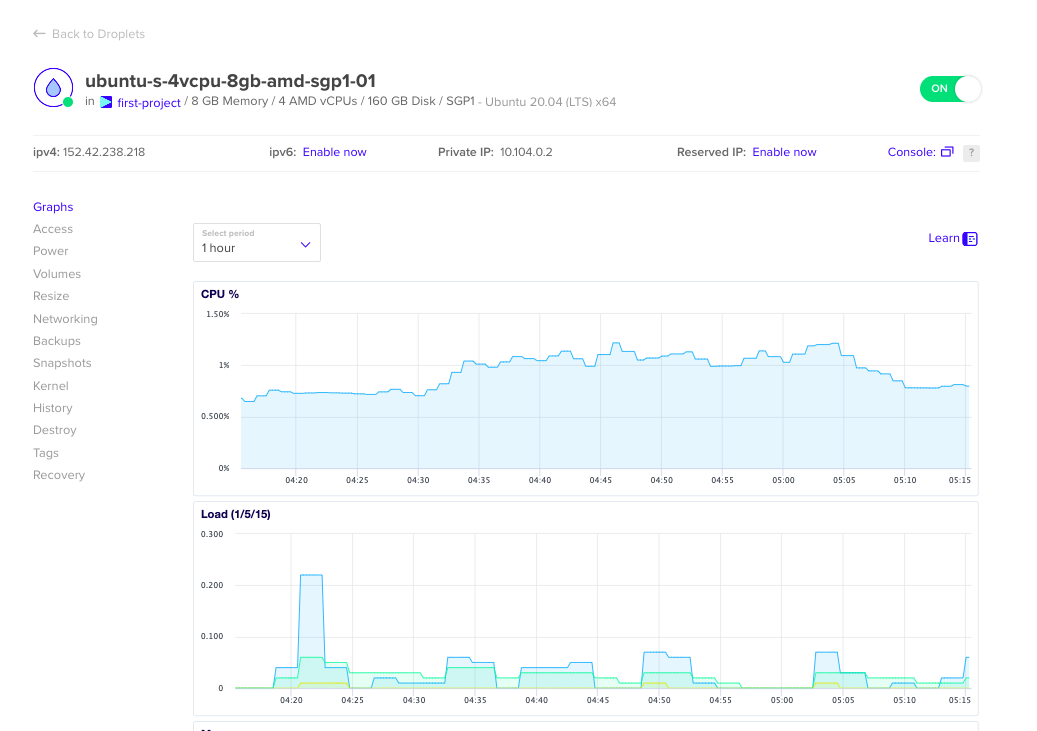
\includegraphics[width=1\textwidth]{figures/ch04/00-tampilan-digitalocean}
    \caption{Tampilan Dasbor VM DigitalOcean}
    \label{fig:00-tampilan-digitalocean}
\end{figure}


\section{Pemasangan dan Konfigurasi Perangkat Lunak}
Penelitian ini membandingkan kinerja Hadoop dan Spark pada \textit{platform cloud} DigitalOcean menggunakan alat pengujian data besar yang bernama HiBench pada lingkup \textit{Micro Benchmarks}, yaitu \textit{Word Count} dan \textit{Sort} dengan data masukan berupa teks yang dibuat oleh \textit{data generation} pada tahap persiapan. 

Sebelum memulai eksperimen, serangkaian pemeriksaan dilakukan untuk memastikan bahwa semua perangkat lunak yang terlibat berfungsi dengan baik. Tahapan ini penting untuk menjamin validitas hasil penelitian. Berikut adalah pemeriksaan yang dilakukan, yaitu
\begin{enumerate}
	\item \textbf{Pengecekan versi Hadoop}. Versi Hadoop yang digunakan dalam penelitian ini adalah 2.4.0. Verifikasi versi dilakukan melalui perintah \textit{hadoop version}, seperti yang ditunjukkan pada Gambar \ref{fig:versi-hadoop}. 
		\begin{figure}[h]
		    \centering
		    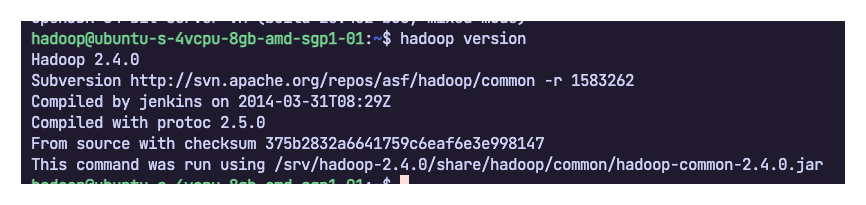
\includegraphics[width=0.8\textwidth]{figures/ch04/versi-hadoop}
		    \caption{Pengecekan Versi Hadoop}
		    \label{fig:versi-hadoop}
		\end{figure}
	\item \textbf{Pengecekan versi Spark}. Versi Spark yang digunakan adalah 2.1.3. Verifikasi dilakukan dengan perintah \textit{spark-submit --version}, seperti yang ditunjukkan pada Gambar \ref{fig:versi-spark}.
		\begin{figure}[h]
		    \centering
		    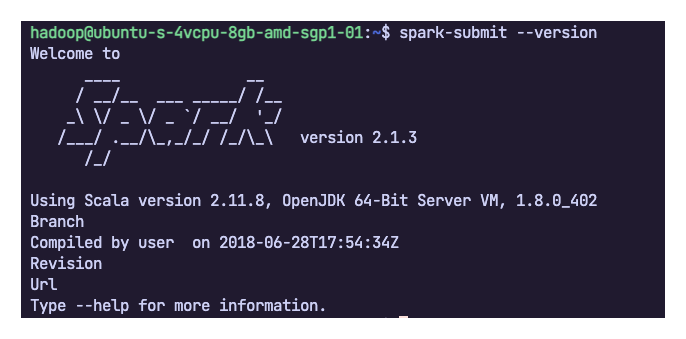
\includegraphics[width=0.8\textwidth]{figures/ch04/versi-spark}
		    \caption{Pengecekan Versi Spark}
		    \label{fig:versi-spark}
		\end{figure}
	\item \textbf{Pemeriksaan \textit{service} yang berjalan ketika beban kerja belum dijalankan}. Status layanan (\textit{services}) yang berjalan pada komputer diperiksa dalam keadaan tanpa beban kerja (\textit{idle}). Layanan yang diharapkan aktif meliputi: Jps, ResourceManager, DataNode, NodeManager, NameNode, dan SecondaryNameNode. Gambar \ref{fig:service-dasar} menunjukkan hasil pemeriksaan layanan dasar.		
		\begin{figure}[h]
		    \centering
		    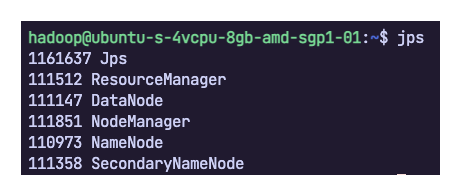
\includegraphics[width=0.8\textwidth]{figures/ch04/service-dasar}
		    \caption{Pengecekan \textit{Service} yang Berjalan (Normal)}
		    \label{fig:service-dasar}
		\end{figure}
	\newpage
	\item \textbf{Pemeriksaan \textit{service} yang berjalan ketika menggunakan Hadoop}. Ketika beban kerja Hadoop dijalankan, layanan tambahan seperti YarnChild, MRAppMaster, dan RunJar  diharapkan aktif, di samping layanan dasar yang telah disebutkan. Gambar \ref{fig:service-hadoop} menunjukkan hasil pemeriksaan layanan saat Hadoop aktif.
		\begin{figure}[h]
		    \centering
		    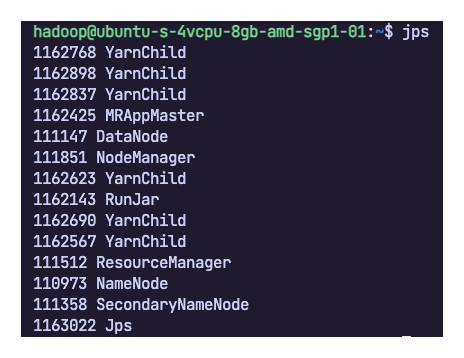
\includegraphics[width=0.7\textwidth]{figures/ch04/service-hadoop}
		    \caption{Pengecekan \textit{Service} yang Berjalan (Hadoop)}
		    \label{fig:service-hadoop}
		\end{figure}
	\item \textbf{Pemeriksaan \textit{service} yang berjalan ketika menggunakan Spark}. Ketika beban kerja Spark dijalankan, layanan seperti CoarseGrainedExecutorBackend, ExecutorLauncher, dan SparkSubmit diharapkan aktif, di samping layanan dasar.  Gambar \ref{fig:service-spark} menunjukkan hasil pemeriksaan layanan saat Spark aktif.
		\begin{figure}[h]
		    \centering
		    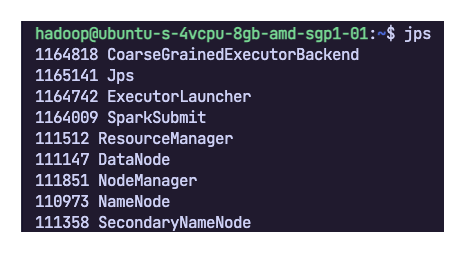
\includegraphics[width=0.8\textwidth]{figures/ch04/service-spark}
		    \caption{Pengecekan \textit{Service} yang Berjalan (Spark)}
		    \label{fig:service-spark}
		\end{figure}
\end{enumerate}

\newpage
\section{Eksperimen}
Selama pengujian, beberapa parameter pada HiBench, Hadoop, dan Spark dikonfigurasi secara tetap untuk menjaga konsistensi dan memungkinkan perbandingan yang adil. Tabel \ref{table:conf-hibench} dan \ref{table:conf-spark} merangkum konfigurasi parameter yang digunakan.

\begin{table}[h]
\caption{Konfigurasi HiBench}
\label{table:conf-hibench}
\scriptsize
\centering
\begin{tabular}{l c p{5cm}} 
\hline
%\multicolumn{1}{c}{\textbf{Nama Parameter}}  & \multicolumn{1}{c}{\textbf{Nilai}} & \multicolumn{1}{c}{\textbf{Keterangan}}  \\ \hline
\textbf{Nama Parameter} & \textbf{Nilai} & \textbf{Keterangan Parameter} \\ \hline
hibench.default.map.parallelism     & 8 & \textit{Mapper numbers} (Hadoop), \textit{partition numbers} (Spark)                          \\
hibench.default.shuffle.parallelism & 8 & \textit{Reducer numbers}  (Hadoop), \textit{shuffle partition} (Spark)\\ \hline                        
\end{tabular}
\end{table}

\begin{table}[h]
\caption{Konfigurasi Spark}
\label{table:conf-spark}
\scriptsize
\centering
\begin{tabular}{l c p{5cm}} 
\hline
\textbf{Nama Parameter} & \textbf{Nilai Parameter} & \textbf{Keterangan Parameter} \\ \hline
hibench.yarn.executor.num & 2 & Jumlah \textit{executor} \\
hibench.yarn.executor.cores & 4 & Jumlah \textit{core} CPU setiap \textit{executor}\\ 
spark.executor.memory & 4G & Jumlah memori setiap \textit{executor} \\
spark.driver.memory & 4G & Jumlah memori tiap \textit{driver} Spark\\ \hline                        
\end{tabular}
\end{table}

Parameter \textit{hibench.default.map.parallelism} memiliki peran yang berbeda pada Hadoop dan Spark. Pada Hadoop, parameter ini menentukan jumlah \textit{Mapper}, yaitu proses yang bertanggung jawab untuk memproses data secara paralel pada tahap \textit{Map}. Pada Spark, parameter ini menentukan jumlah partisi data, yaitu unit pemrosesan dasar dalam Spark.

Parameter \textit{hibench.default.shuffle.parallelism} juga memiliki peran yang berbeda pada Hadoop dan Spark. Pada Hadoop, parameter ini menentukan jumlah \textit{Reducer}, yaitu proses yang bertanggung jawab untuk menggabungkan hasil dari tahap \textit{Map}. Pada Spark, parameter ini menentukan jumlah \textit{Shuffle partition}, yaitu jumlah partisi data yang digunakan selama tahap \textit{Shuffle}, yaitu proses pengocokan dan pengurutan data antara tahap \textit{Map} dan \textit{Reduce}.

%Berikut penjelasan mengenai parameter Spark pada Tabel \ref{table:conf-spark}:
%\begin{enumerate}
%	\item \textbf{hibench.yarn.executor.num}: Parameter ini menentukan jumlah \textit{executor} yang akan dialokasikan untuk aplikasi Spark. \textit{Executor} adalah proses yang berjalan pada node pekerja (\textit{worker node}) di kluster YARN dan bertanggung jawab untuk menjalankan task Spark.
%	\item \textbf{hibench.yarn.executor.cores}: Parameter ini menentukan jumlah core CPU yang dialokasikan untuk setiap \textit{executor}. Semakin banyak core yang dialokasikan, semakin banyak task yang dapat dijalankan secara paralel oleh setiap \textit{executor}.
%	\item \textbf{spark.executor.memory}: Parameter ini menentukan jumlah memori yang dialokasikan untuk setiap \textit{executor}. Memori ini digunakan untuk menyimpan data yang diproses oleh \textit{executor}, seperti RDD dan data yang di-\textit{cache}.
%	\item \textbf{spark.driver.memory}: Parameter ini menentukan jumlah memori yang dialokasikan untuk proses driver Spark. Driver bertanggung jawab untuk mengelola aplikasi Spark, menjadwalkan task, dan mengumpulkan hasil.
%\end{enumerate}

\section{Data Keluaran yang Dihasilkan}

Setiap pengujian akan menghasilkan berkas output berupa data HiBench \textit{Report} dan Dool \textit{System Monitoring}. Data HiBench \textit{Report} akan terlihat seperti pada Gambar \ref{fig:data-hibench-report}. Pada Gambar tersebut, terlihat bahwa ekstensi berkasnya \textit{.report} dan terlihat beberapa data seperti jenis beban kerja, aplikasi yang digunakan, besar input data, durasi, dan \textit{throughput}.

\begin{figure}[h]
    \centering
    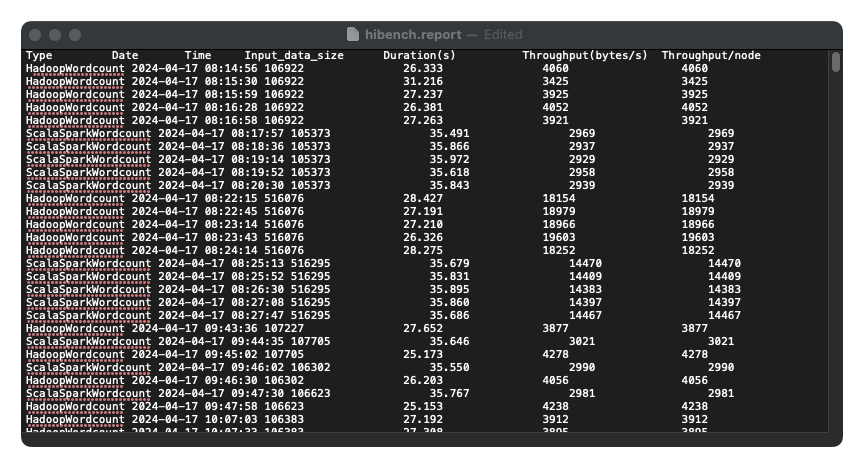
\includegraphics[width=0.9\textwidth]{figures/ch04/data-hibench}
    \caption{Data HiBench \textit{Report}}
    \label{fig:data-hibench-report}
\end{figure}

Dool, alat monitoring sistem, menghasilkan berkas CSV (\textit{comma-separated value}) untuk setiap perulangan eksperimen. Dengan demikian, terdapat sekitar 240 berkas CSV, seperti yang ditunjukkan pada Gambar \ref{fig:data-dool-luar}. Penamaan berkas mengikuti format: [jenis beban kerja]-[ukuran data]-[nomor perulangan]-[aplikasi]. Sebagai contoh, \textit{sort-fivegig-1-hadoop.csv} menunjukkan \textit{data monitoring} untuk beban kerja sort, data masukan 5 GB, perulangan pertama, dan aplikasi Hadoop.

\begin{figure}[h]
    \centering
    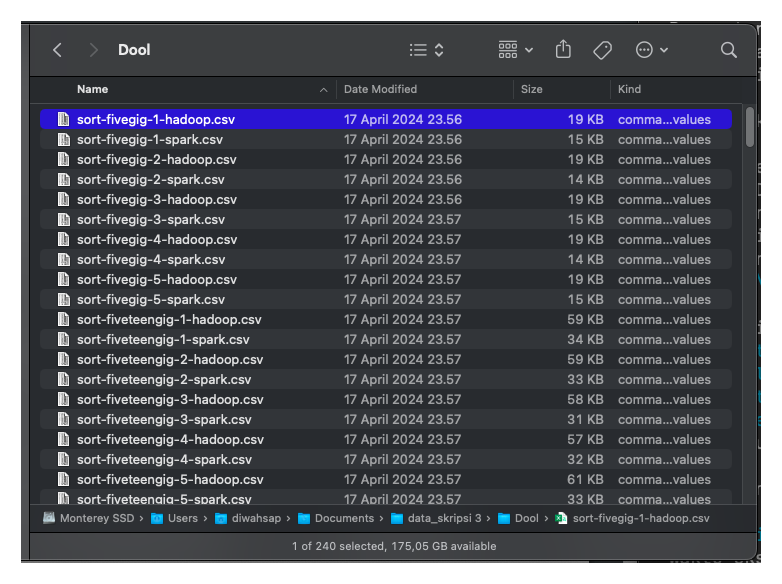
\includegraphics[width=0.75\textwidth]{figures/ch04/data-dool-luar}
    \caption{Berkas Dool}
    \label{fig:data-dool-luar}
\end{figure}

Struktur data Dool, yang ditunjukkan pada Gambar \ref{fig:data-dool-dalam}, mencakup baris \textit{header} (baris 1-4) dan nama kolom (baris 6). Data ini akan dianalisis lebih lanjut untuk mendapatkan \textit{insight} tentang kinerja Hadoop dan Spark.

\begin{landscape}
\begin{figure}[h]
    \centering
    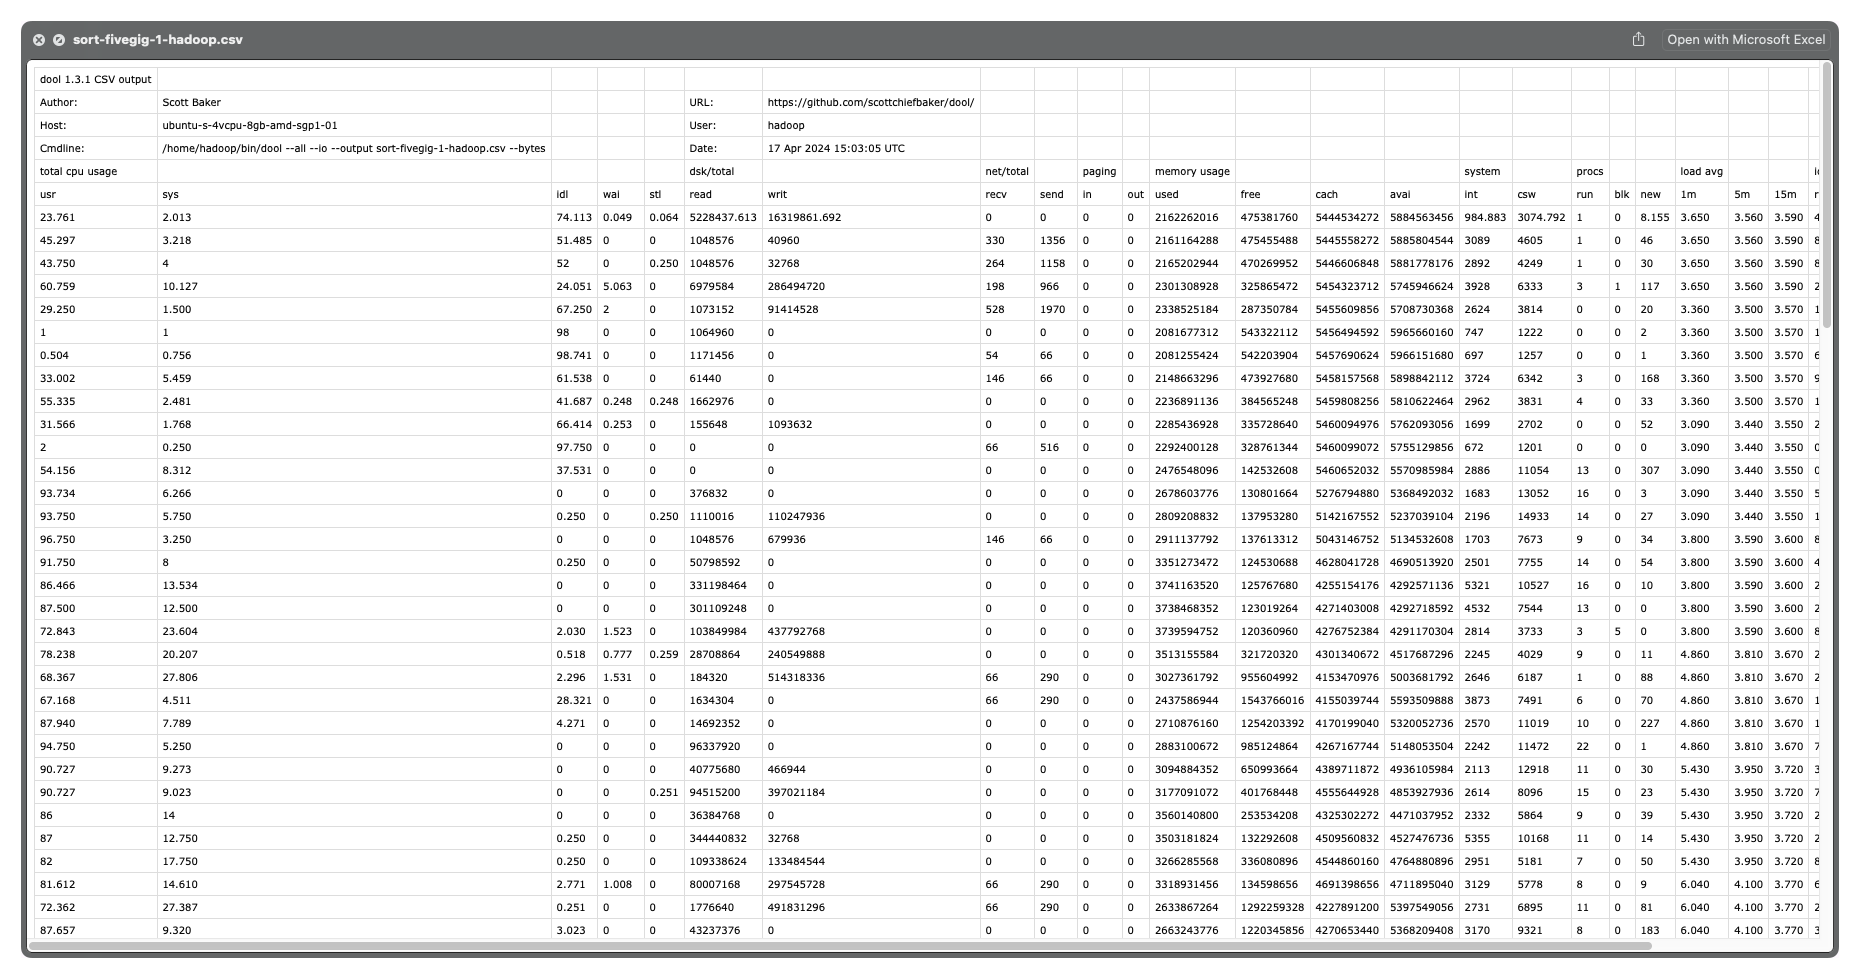
\includegraphics[width=\linewidth, height=0.5\linewidth]{figures/ch04/data-dool-dalam}
    \caption{Contoh Data Dool}
    \label{fig:data-dool-dalam}
\end{figure}
\end{landscape}

\newpage
\section {Analisis dan Evaluasi Hasil Eksperimen: Kinerja}
\subsection{Persebaran Waktu Eksekusi pada Hadoop dan Spark}
Waktu eksekusi adalah durasi yang diperlukan untuk memproses data. Nilai parameter ini diperoleh dengan menghitung selisih antara waktu awal dan waktu akhir saat Apache Hadoop dan Apache Spark dijalankan atau dihentikan untuk memproses input data dengan beban kerja masing-masing. Satuan pengukuran untuk parameter waktu eksekusi adalah detik. Setiap beban kerja dilakukan sebanyak lima kali pengulangan untuk mendapatkan hasil yang lebih akurat dan representatif.

Gambar \ref{fig:lama-waktu-eksekusi-sort} dan \ref{fig:lama-waktu-eksekusi-wordcount} menyajikan \textit{scatter plot} yang membandingkan performa Hadoop dan Spark dalam dua tugas pemrosesan data yang berbeda, yaitu \textit{sort} dan \textit{word count}. Sumbu x pada kedua gambar menunjukkan variasi ukuran input data, mulai dari 100 KB hingga 15 GB, sementara sumbu y menunjukkan waktu eksekusi dalam detik.

\begin{figure}[h]
    \centering
    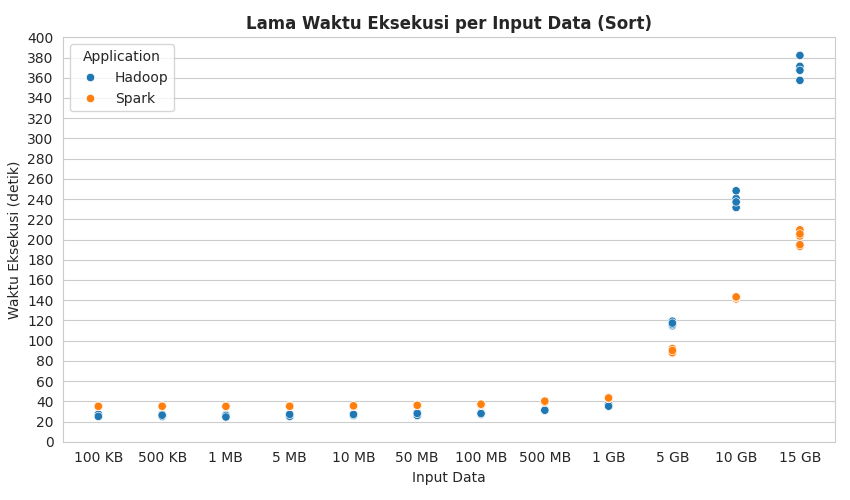
\includegraphics[width=1\textwidth]{figures/ch04/1-lama-waktu-eksekusi-sort.png}
    \caption{Persebaran Waktu Eksekusi \textit{Sort} (Hadoop, Spark)}
    \label{fig:lama-waktu-eksekusi-sort}
\end{figure}

Pada Gambar \ref{fig:lama-waktu-eksekusi-sort}, terlihat bahwa waktu eksekusi Hadoop untuk input data 100 KB hingga 1 GB secara konsisten lebih cepat dibandingkan Spark. Hadoop berada pada rentang waktu 20-40 detik, sedangkan Spark berada pada rentang waktu 35-45 detik.

Namun, untuk input data sebesar 5 GB, Spark menunjukkan waktu eksekusi yang lebih cepat dibandingkan Hadoop. Spark berada pada rentang 80-100 detik, sementara Hadoop berada pada rentang 110-125 detik. Perbedaan performa ini semakin signifikan seiring bertambahnya ukuran data, terutama pada ukuran data 10 GB dan 15 GB. Perbedaan waktu eksekusi antara Hadoop dan Spark semakin jauh pada beban kerja \textit{sort} dengan ukuran data yang lebih besar.

\begin{figure}[h]
    \centering
    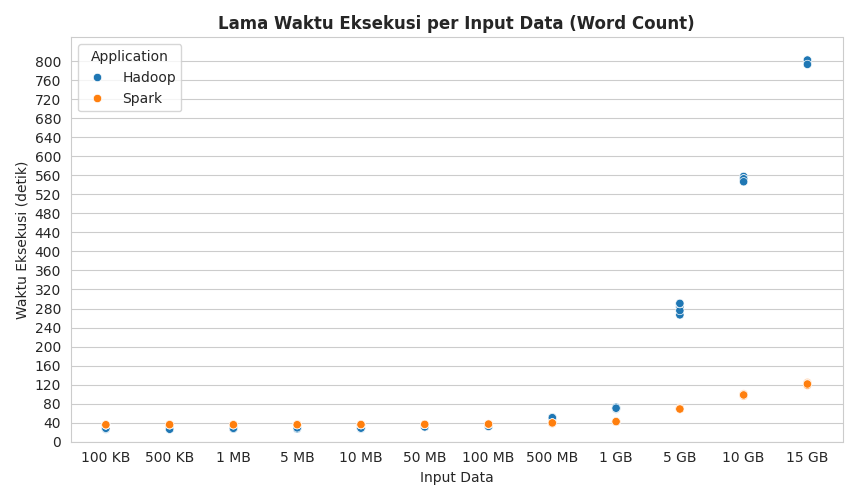
\includegraphics[width=1\textwidth]{figures/ch04/1-lama-waktu-eksekusi-wordcount.png}
    \caption{Persebaran Waktu Eksekusi \textit{Word Count} (Hadoop, Spark)}
    \label{fig:lama-waktu-eksekusi-wordcount}
\end{figure}

Pada Gambar \ref{fig:lama-waktu-eksekusi-wordcount}, Spark menunjukkan performa yang lebih baik dibandingkan Hadoop untuk ukuran input data 500 MB, 1 GB, 5 GB, 10 GB, dan 15 GB pada beban kerja \textit{word count}. Namun, untuk ukuran input data 100 KB hingga 100 MB, Hadoop masih lebih unggul. Waktu eksekusi Hadoop untuk input data 100 KB hingga 100 MB berada pada rentang 20-40 detik, meskipun perbedaannya tidak signifikan dibandingkan Spark karena titik data Hadoop dan Spark saling berdekatan.

Hasil ini menunjukkan bahwa Spark lebih unggul dan konsisten dibandingkan Hadoop dalam menangani tugas pemrosesan data yang lebih besar, dengan rincian sebagai berikut:
\begin{enumerate}
\item Untuk beban kerja \textit{sort}, Spark lebih unggul mulai dari ukuran input data 5 GB, 10 GB, dan 15 GB.
\item Untuk beban kerja \textit{word count}, Spark lebih unggul mulai dari ukuran input data 500 MB, 1 GB, 5 GB, 10 GB, dan 15 GB.
\end{enumerate}

Secara keseluruhan, Spark menunjukkan kinerja yang lebih baik dalam menangani data berukuran besar, sementara Hadoop lebih efisien untuk data berukuran kecil hingga menengah.

% ----------------------------------------
\subsection {Persebaran \textit{Throughput} pada Hadoop dan Spark}

\textit{Throughput} adalah kecepatan pertukaran data per detik. Kegiatan pertukaran data tersebut terjadi pada \textit{node} yang dipakai dalam komputer komputasi, saat Hadoop maupun Spark memproses data. Oleh karena itu, semakin tinggi nilai \textit{throughput}, semakin sedikit waktu yang dibutuhkan untuk menyelesaikan komputasi. Satuan \textit{throughput} pada penelitian ini adalah MB/s (mega bita per detik).

Gambar di bawah akan menyajikan \textit{scatter plot} yang membandingkan \textit{throughput} Hadoop dan Spark dalam dua tugas pemrosesan data, yaitu \textit{sort} (Gambar \ref{fig:throughput-sort}) dan \textit{word count} (Gambar \ref{fig:throughput-wordcount}). Sumbu x pada kedua gambar menunjukkan variasi ukuran input data, sedangkan sumbu y menunjukkan \textit{throughput} dalam MB/s.

\begin{figure}[h]
    \centering
    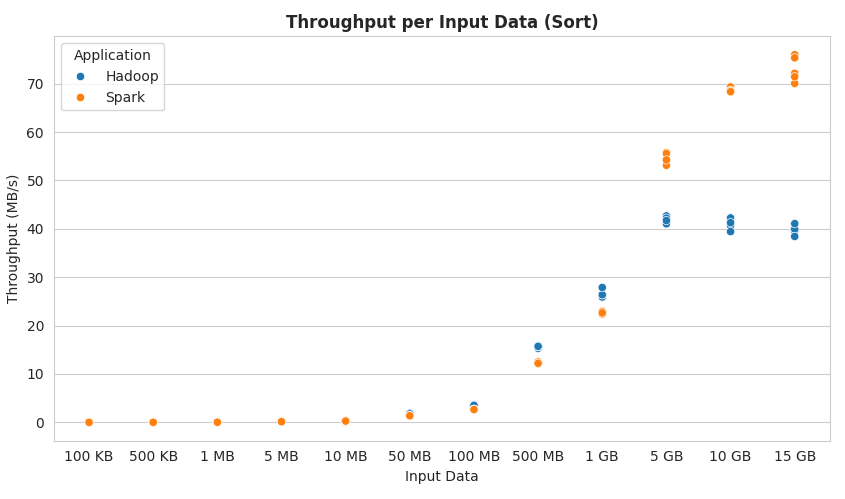
\includegraphics[width=1\textwidth]{figures/ch04/1-throughput-sort.png}
    \caption{\textit{Throughput Sort} (Hadoop, Spark)}
    \label{fig:throughput-sort}
\end{figure}

Pada tugas \textit{sort} (Gambar \ref{fig:throughput-sort}), Spark menunjukkan peningkatan \textit{throughput} yang signifikan seiring dengan bertambahnya ukuran data. Pada ukuran data terbesar (15 GB), Spark mencapai \textit{throughput} sekitar 70 MB/s. Sebaliknya, Hadoop menunjukkan peningkatan \textit{throughput} yang lebih lambat dan hanya mencapai sekitar 40 MB/s pada ukuran data yang sama. Hal ini menunjukkan bahwa Spark mampu melakukan pertukaran data yang lebih besar daripada Hadoop.

\begin{figure}[h]
    \centering
    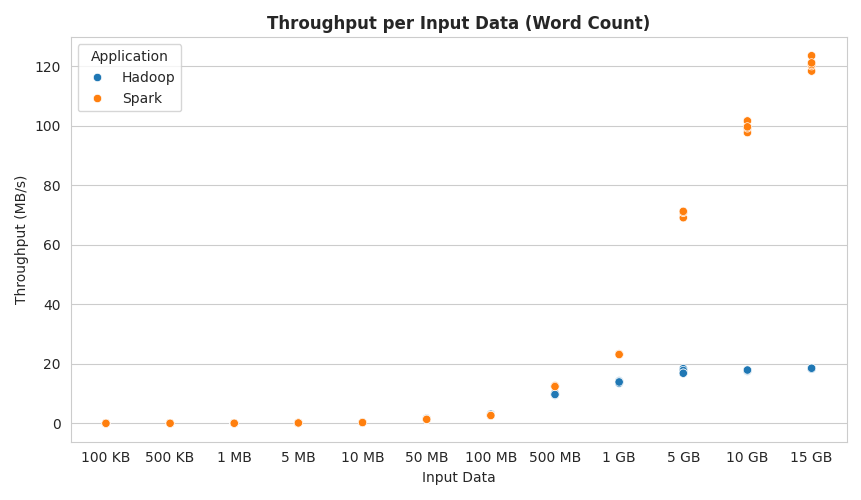
\includegraphics[width=1\textwidth]{figures/ch04/1-throughput-wordcount.png}
    \caption{\textit{Throughput Word Count} (Hadoop, Spark)}
    \label{fig:throughput-wordcount}
\end{figure}

Pada tugas \textit{word count} (Gambar \ref{fig:throughput-wordcount}), Spark mencapai \textit{throughput} yang lebih tinggi daripada Hadoop. Perbedaan \textit{throughput} paling mencolok terlihat pada ukuran data terbesar (15 GB), di mana Spark mencapai \textit{throughput} lebih dari 120 MB/s, sedangkan Hadoop hanya mencapai sekitar 20 MB/s. Meskipun Spark menunjukkan peningkatan \textit{throughput} yang signifikan pada ukuran data besar (1 GB, 5 GB, 10 GB, dan 15 GB), pada data input yang lebih kecil, 100 KB sampai 100 MB, perbedaan \textit{throughput} antara Hadoop dan Spark tidak berbeda jauh untuk \textit{word count}.

Hasil ini menunjukkan bahwa Spark lebih unggul dalam menangani data berukuran besar untuk kedua tugas pemrosesan data tersebut. Spark mampu mempertahankan \textit{throughput} yang lebih tinggi dibandingkan Hadoop, terutama saat menangani data berukuran besar, dengan rincian sebagai berikut:
\begin{enumerate}
\item Untuk beban kerja \textit{sort}, Spark lebih unggul pada ukuran data 1 GB, 5 GB, 10 GB, dan 15 GB.
\item Untuk beban kerja \textit{word count}, Spark lebih unggul pada ukuran data 1 GB, 5 GB, 10 GB, dan 15 GB.
\end{enumerate}

Secara keseluruhan, Spark menunjukkan kinerja yang lebih baik dalam hal \textit{throughput} terutama pada data berukuran besar, sementara Hadoop masih menunjukkan performa yang kompetitif pada data berukuran kecil hingga menengah.

% ----------------------------------------

\subsection {Rata-rata Waktu Eksekusi pada Hadoop dan Spark}

Gambar \ref{fig:mean-dur-sort} dan \ref{fig:mean-dur-wordcount} menyajikan \textit{line plot} yang menggambarkan rata-rata waktu eksekusi Hadoop dan Spark untuk tugas \textit{sort} dan \textit{word count} dengan berbagai ukuran data. Sumbu x pada kedua gambar menunjukkan ukuran input data, sedangkan sumbu y menunjukkan rata-rata waktu eksekusi dalam detik. Garis vertikal pada kedua gambar menunjukkan titik di mana Spark mulai menunjukkan performa yang lebih cepat dibandingkan Hadoop.

\begin{figure}[h]
    \centering
    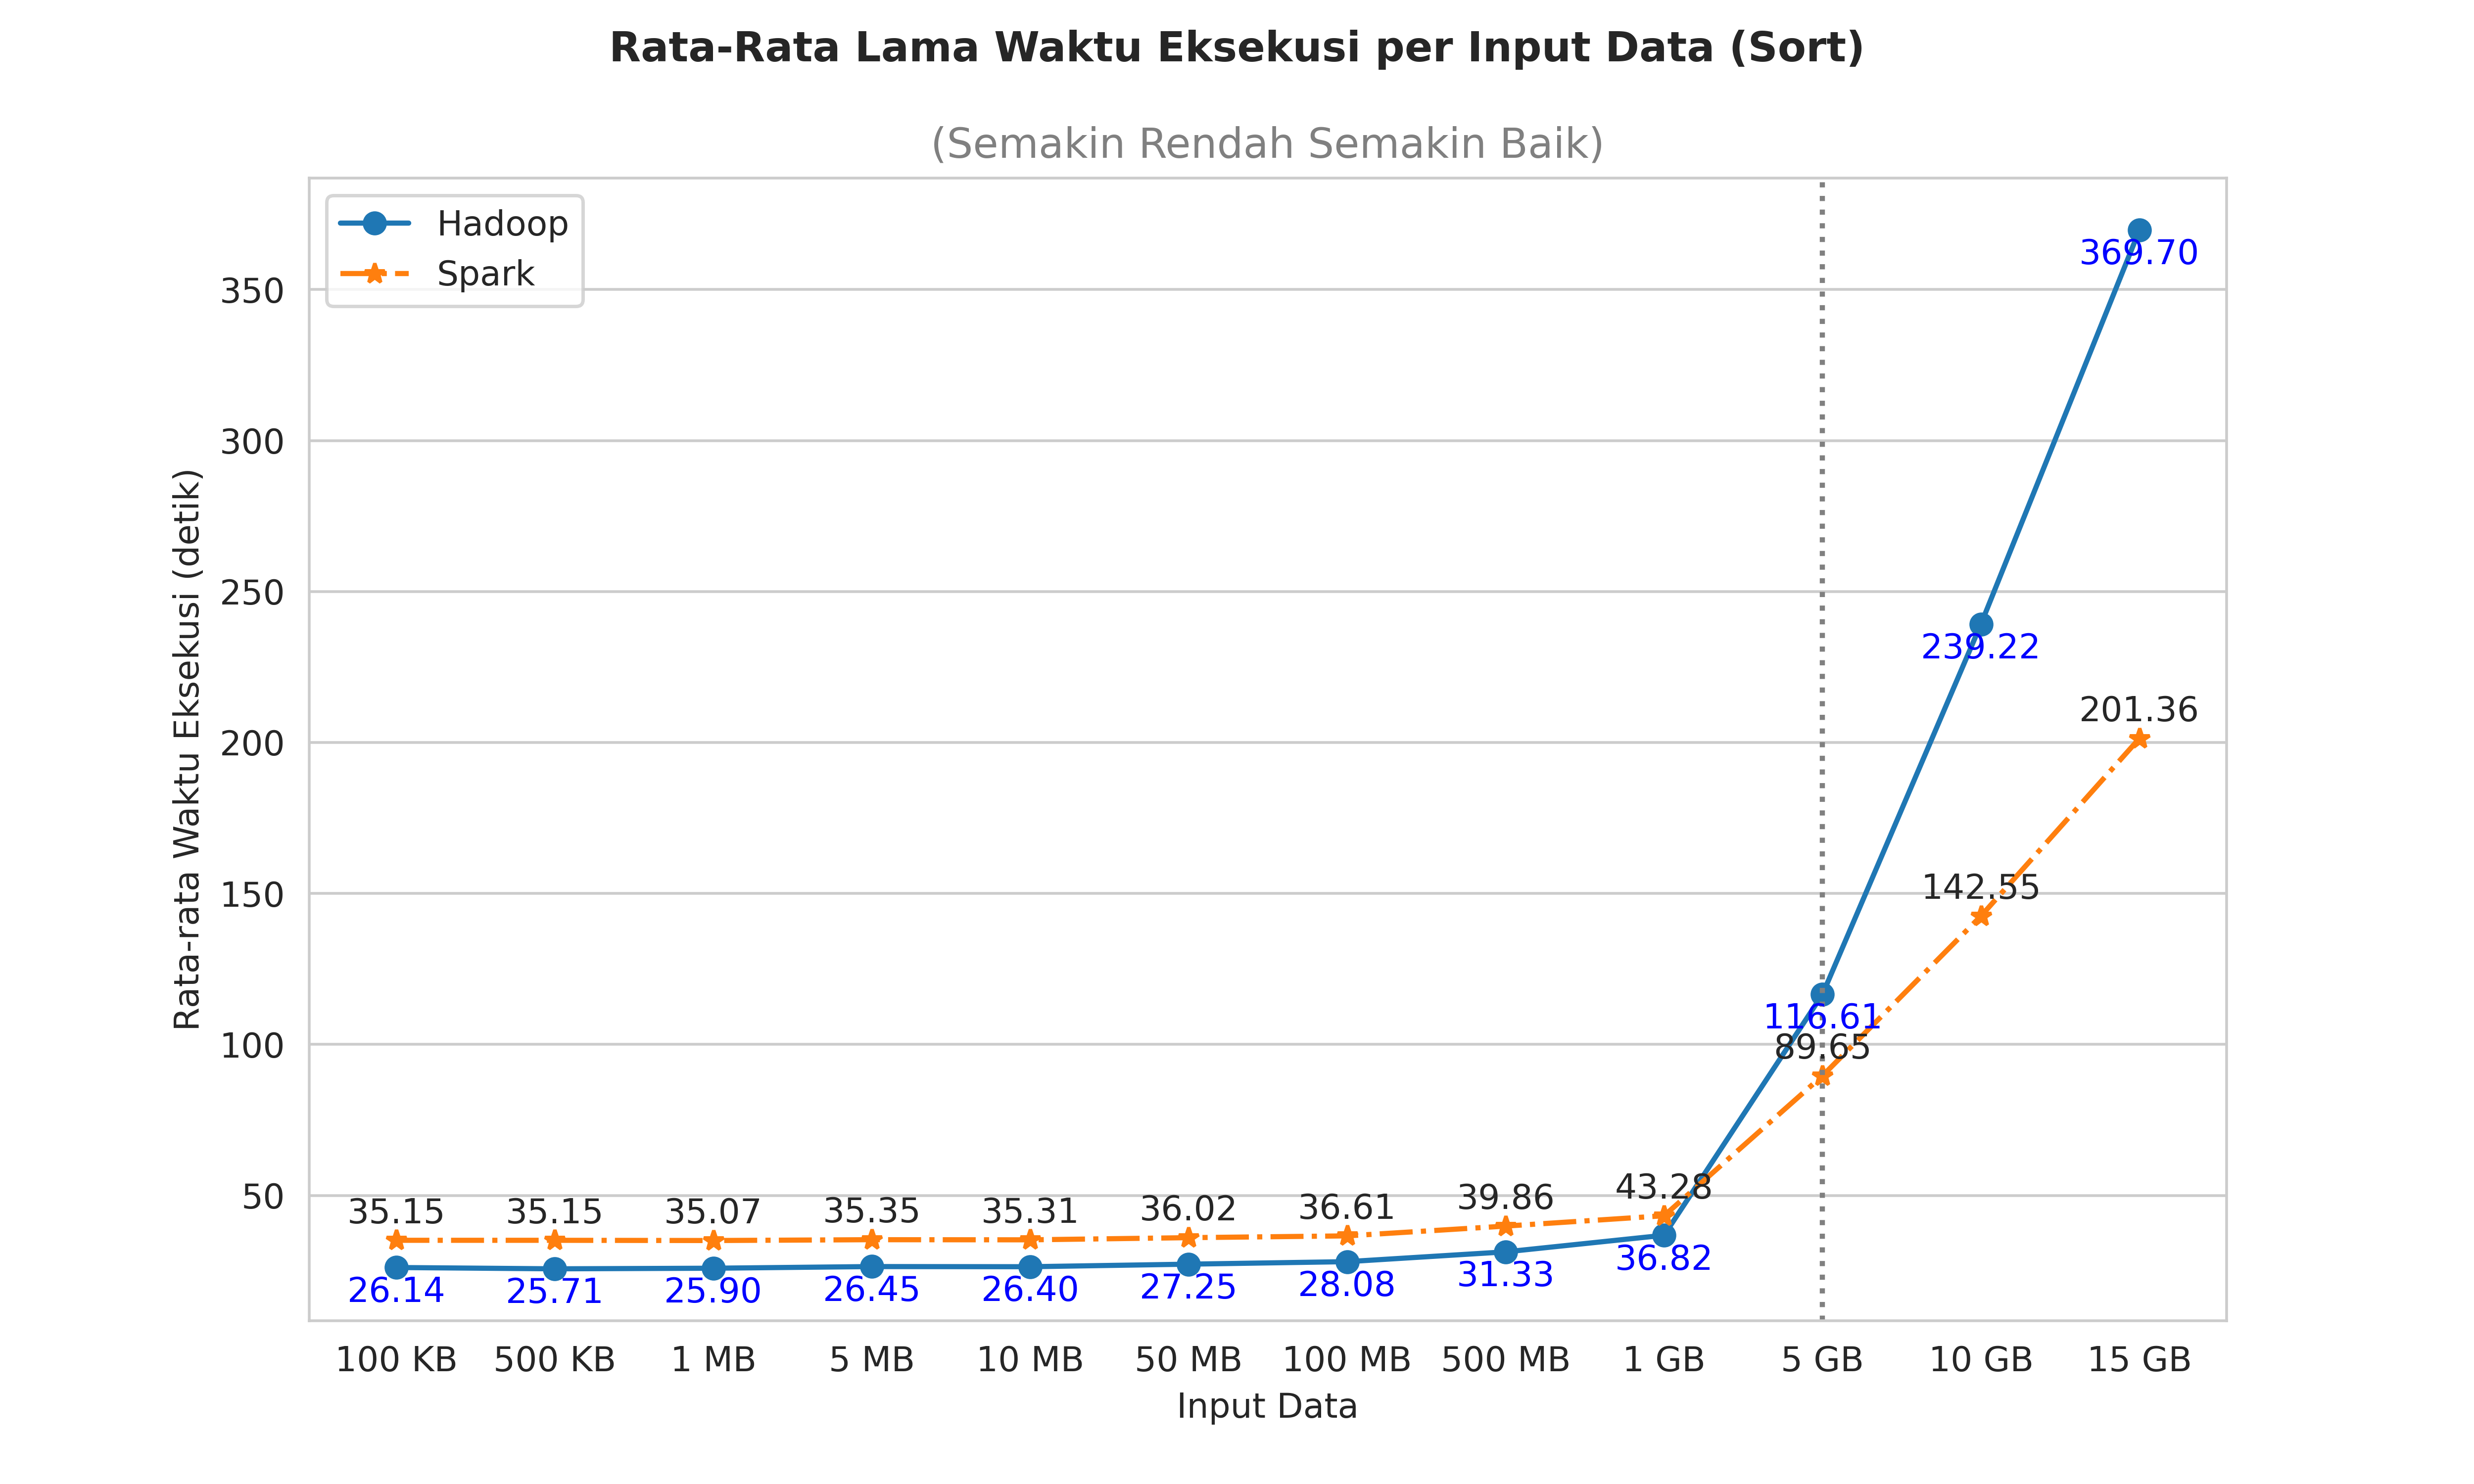
\includegraphics[width=1\textwidth]{figures/ch04/2-mean-lama-waktu-eksekusi-sort.png}
    \caption{Rata-rata Waktu Eksekusi \textit{(Sort)}}
    \label{fig:mean-dur-sort}
\end{figure}

Pada Gambar \ref{fig:mean-dur-sort}, terlihat bahwa Hadoop secara konsisten memiliki waktu eksekusi yang lebih rendah daripada Spark untuk ukuran input data 100 KB-1 GB pada tugas \textit{sort}. Perbedaan performa mulai terlihat pada input data 5 GB, di mana waktu eksekusi pada Hadoop mulai meningkat secara eksponensial, sementara Spark menunjukkan kenaikan yang lebih moderat. Pada ukuran data terbesar (15 GB), waktu eksekusi Hadoop mencapai sekitar 369,70 detik, sedangkan Spark hanya mencapai sekitar 201,36 detik.

\begin{figure}[h]
    \centering
    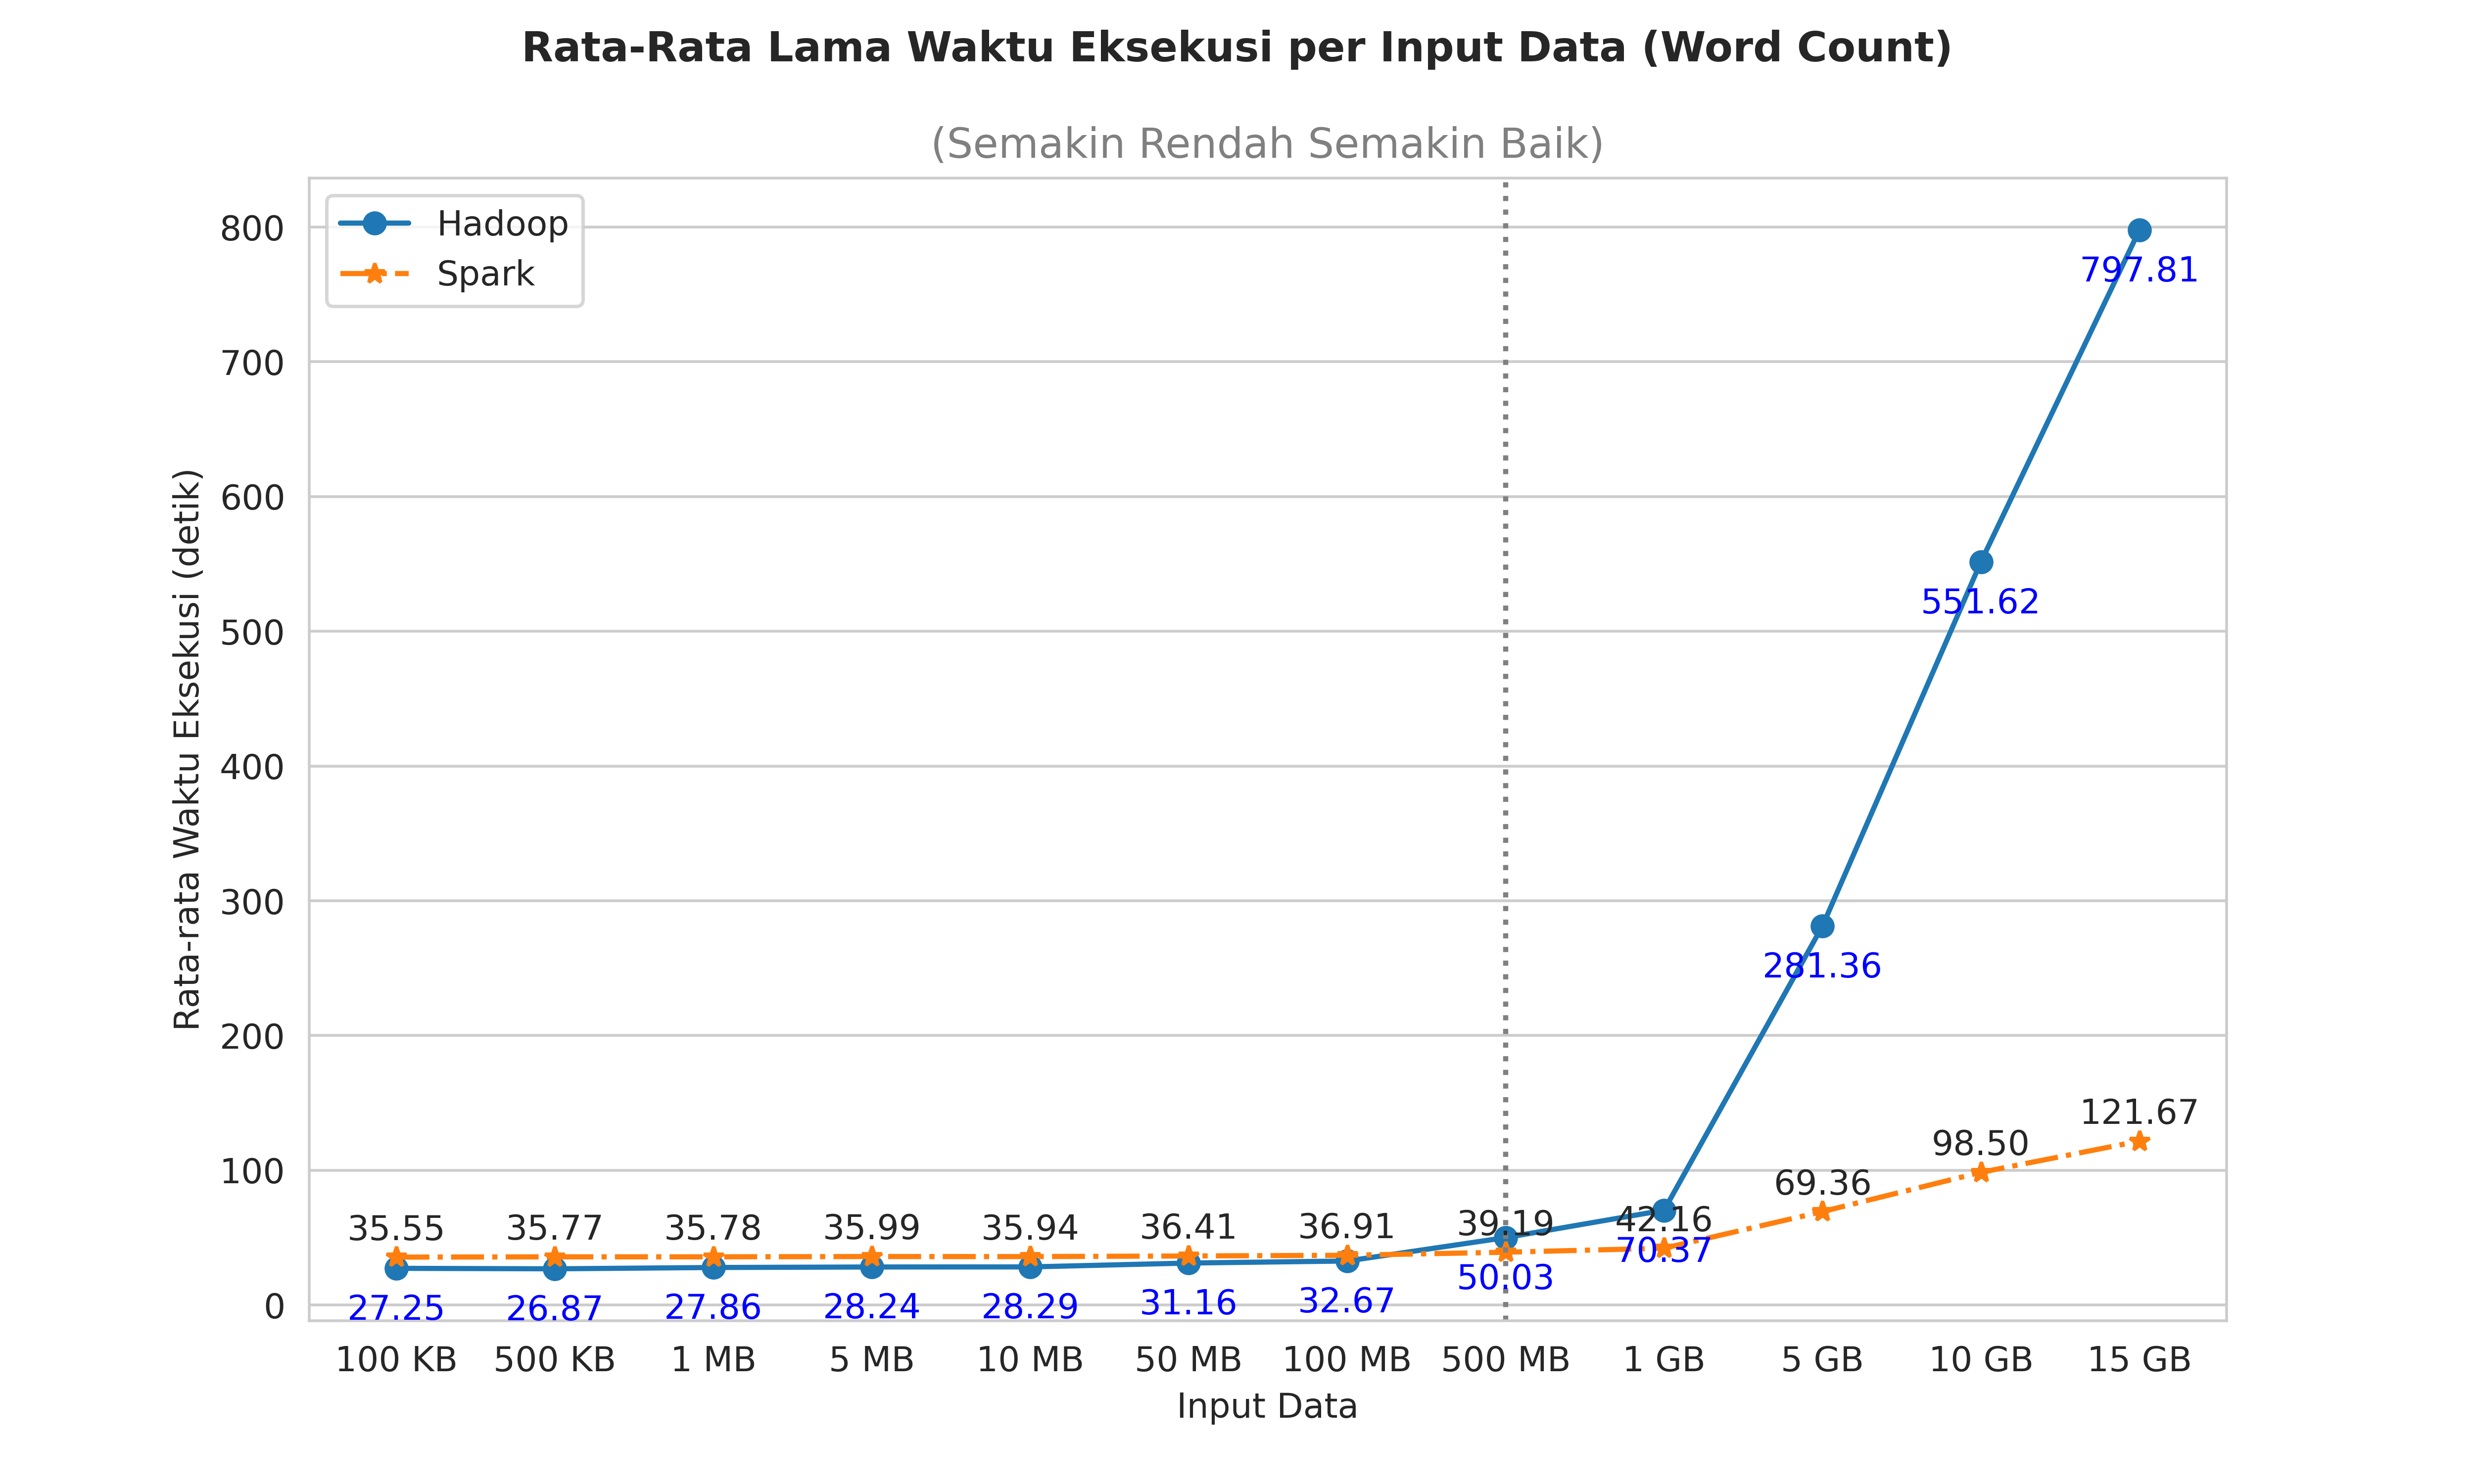
\includegraphics[width=1\textwidth]{figures/ch04/2-mean-lama-waktu-eksekusi-wordcount.png}
    \caption{Rata-rata Waktu Eksekusi \textit{(Word Count)}}
    \label{fig:mean-dur-wordcount}
\end{figure}

Pada Gambar \ref{fig:mean-dur-wordcount}, Spark juga menunjukkan performa yang lebih baik daripada Hadoop pada sebagian besar ukuran data pada tugas \textit{word count}, khususnya mulai dari input data 500 MB sampai 15 GB. Lama waktu eksekusi beban kerja pada Hadoop mulai mengalami kenaikan sejak input data 500 MB. Sedangkan, Spark baru mengalami kenaikan waktu eksekusi pada input data 5 GB. Pada ukuran data terbesar (15 GB), waktu eksekusi Hadoop mencapai sekitar 797,81 detik, sedangkan Spark hanya mencapai sekitar 121,67 detik.

Hasil ini menunjukkan bahwa Spark lebih unggul dalam menangani data berukuran besar untuk kedua tugas pemrosesan data tersebut. Spark mampu mempertahankan waktu eksekusi yang lebih rendah dibandingkan Hadoop, terutama saat menangani data berukuran besar, dengan rincian sebagai berikut:
\begin{enumerate}
\item Untuk beban kerja \textit{sort}, Hadoop lebih unggul pada ukuran data 100 KB hingga 1 GB, sedangkan Spark mulai unggul pada ukuran data 5 GB dan seterusnya.
\item Untuk beban kerja \textit{word count}, Spark lebih unggul pada ukuran data 500 MB hingga 15 GB.
\end{enumerate}

Secara keseluruhan, Spark menunjukkan kinerja yang lebih baik dalam hal waktu eksekusi terutama pada data berukuran besar, sementara Hadoop masih menunjukkan performa yang kompetitif pada data berukuran kecil hingga menengah.


% ----------------------------------------

\subsection {Rata-rata \textit{Throughput} pada Hadoop dan Spark}

Gambar \ref{fig:mean-throughput-sort} dan \ref{fig:mean-throughput-wordcount} menyajikan \textit{line plot} yang menggambarkan rata-rata throughput Hadoop dan Spark untuk tugas \textit{sort} dan \textit{word count} dengan berbagai ukuran data. Sumbu x pada kedua gambar menunjukkan ukuran input data, sedangkan sumbu y menunjukkan rata-rata \textit{throughput} dalam MB/s. Garis vertikal pada kedua gambar menunjukkan titik di mana Spark mulai menunjukkan throughput yang lebih tinggi dibandingkan Hadoop.

\begin{figure}[h]
    \centering
    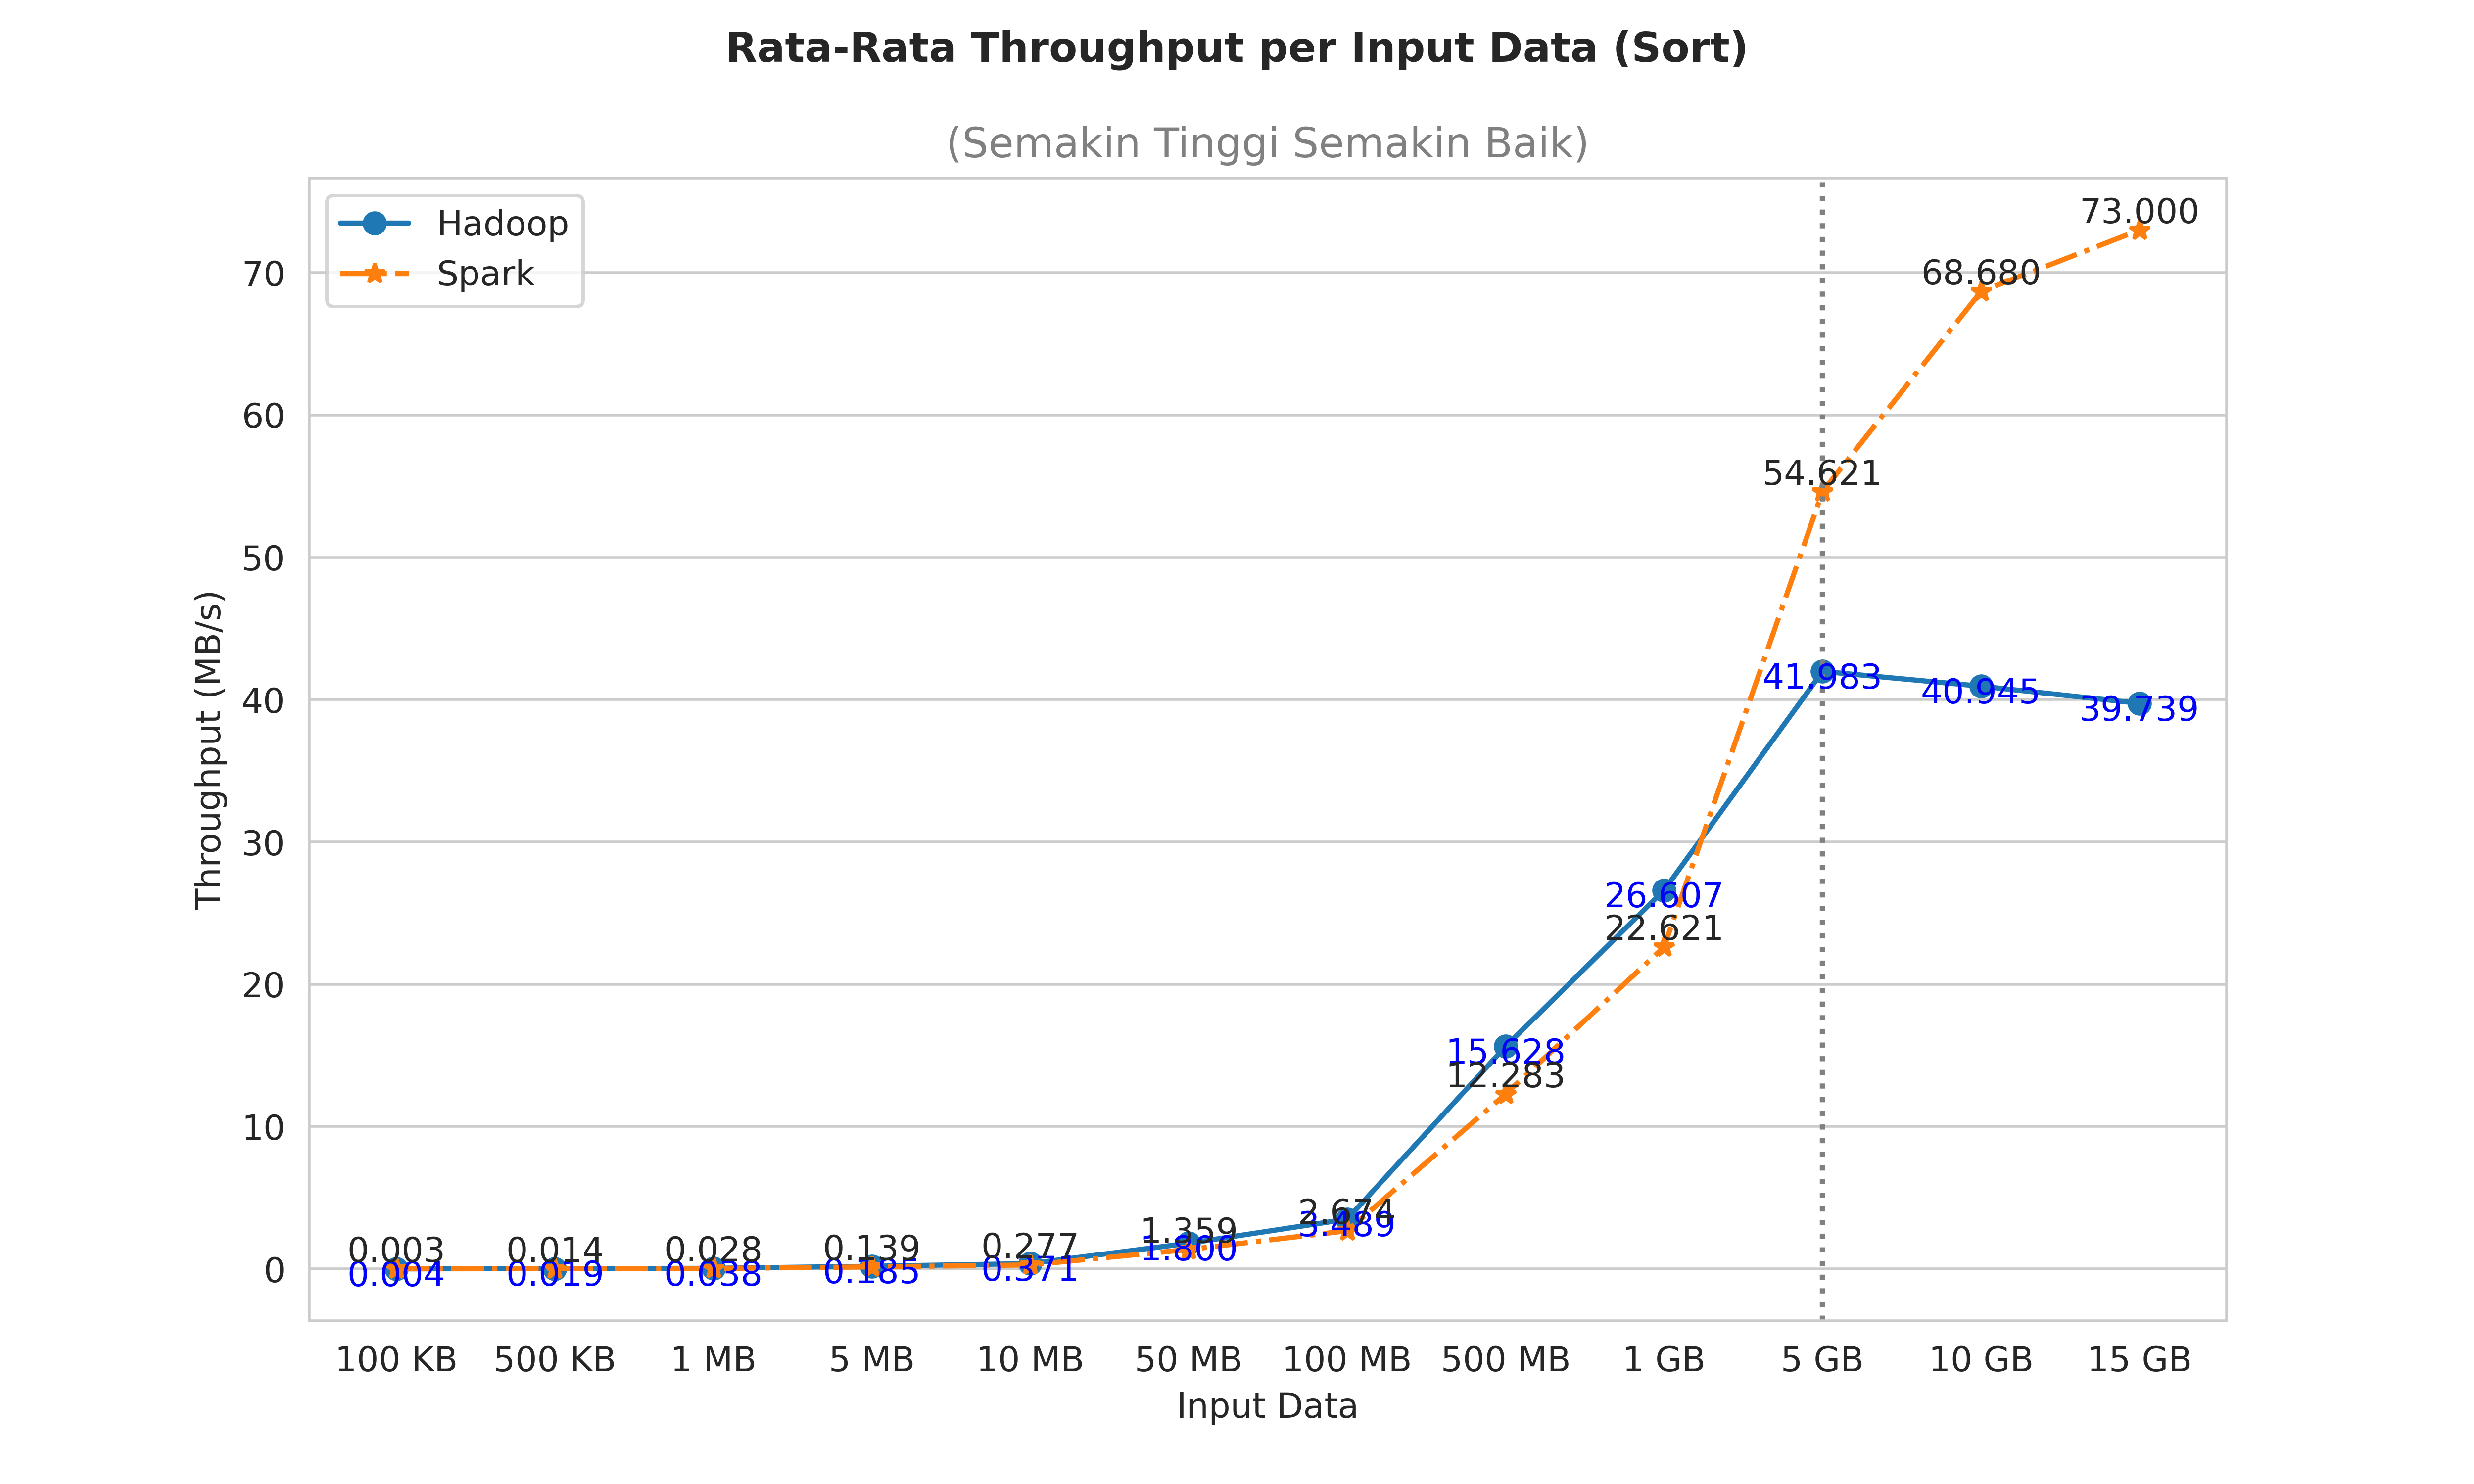
\includegraphics[width=0.95\textwidth]{figures/ch04/2-mean-throughput-sort.png}
    \caption{Rata-rata \textit{Throughput (Sort)}}
    \label{fig:mean-throughput-sort}
\end{figure}

Pada beban kerja \textit{sort}, Spark menunjukkan peningkatan \textit{throughput} yang signifikan seiring dengan meningkatnya ukuran data. Pada ukuran data kecil (di bawah 10 MB), \textit{throughput} Hadoop dan Spark relatif rendah dan sebanding. Setelah input data 10 MB, \textit{throughput} pada Hadoop meningkat dan sedikit menjauhi Spark. Namun, setelah input data 1 GB, Spark secara konsisten menunjukkan throughput yang lebih tinggi, mencapai 73.00 MB/s pada 15 GB dibandingkan dengan 39.74 MB/s untuk Hadoop.

\begin{figure}[h]
    \centering
    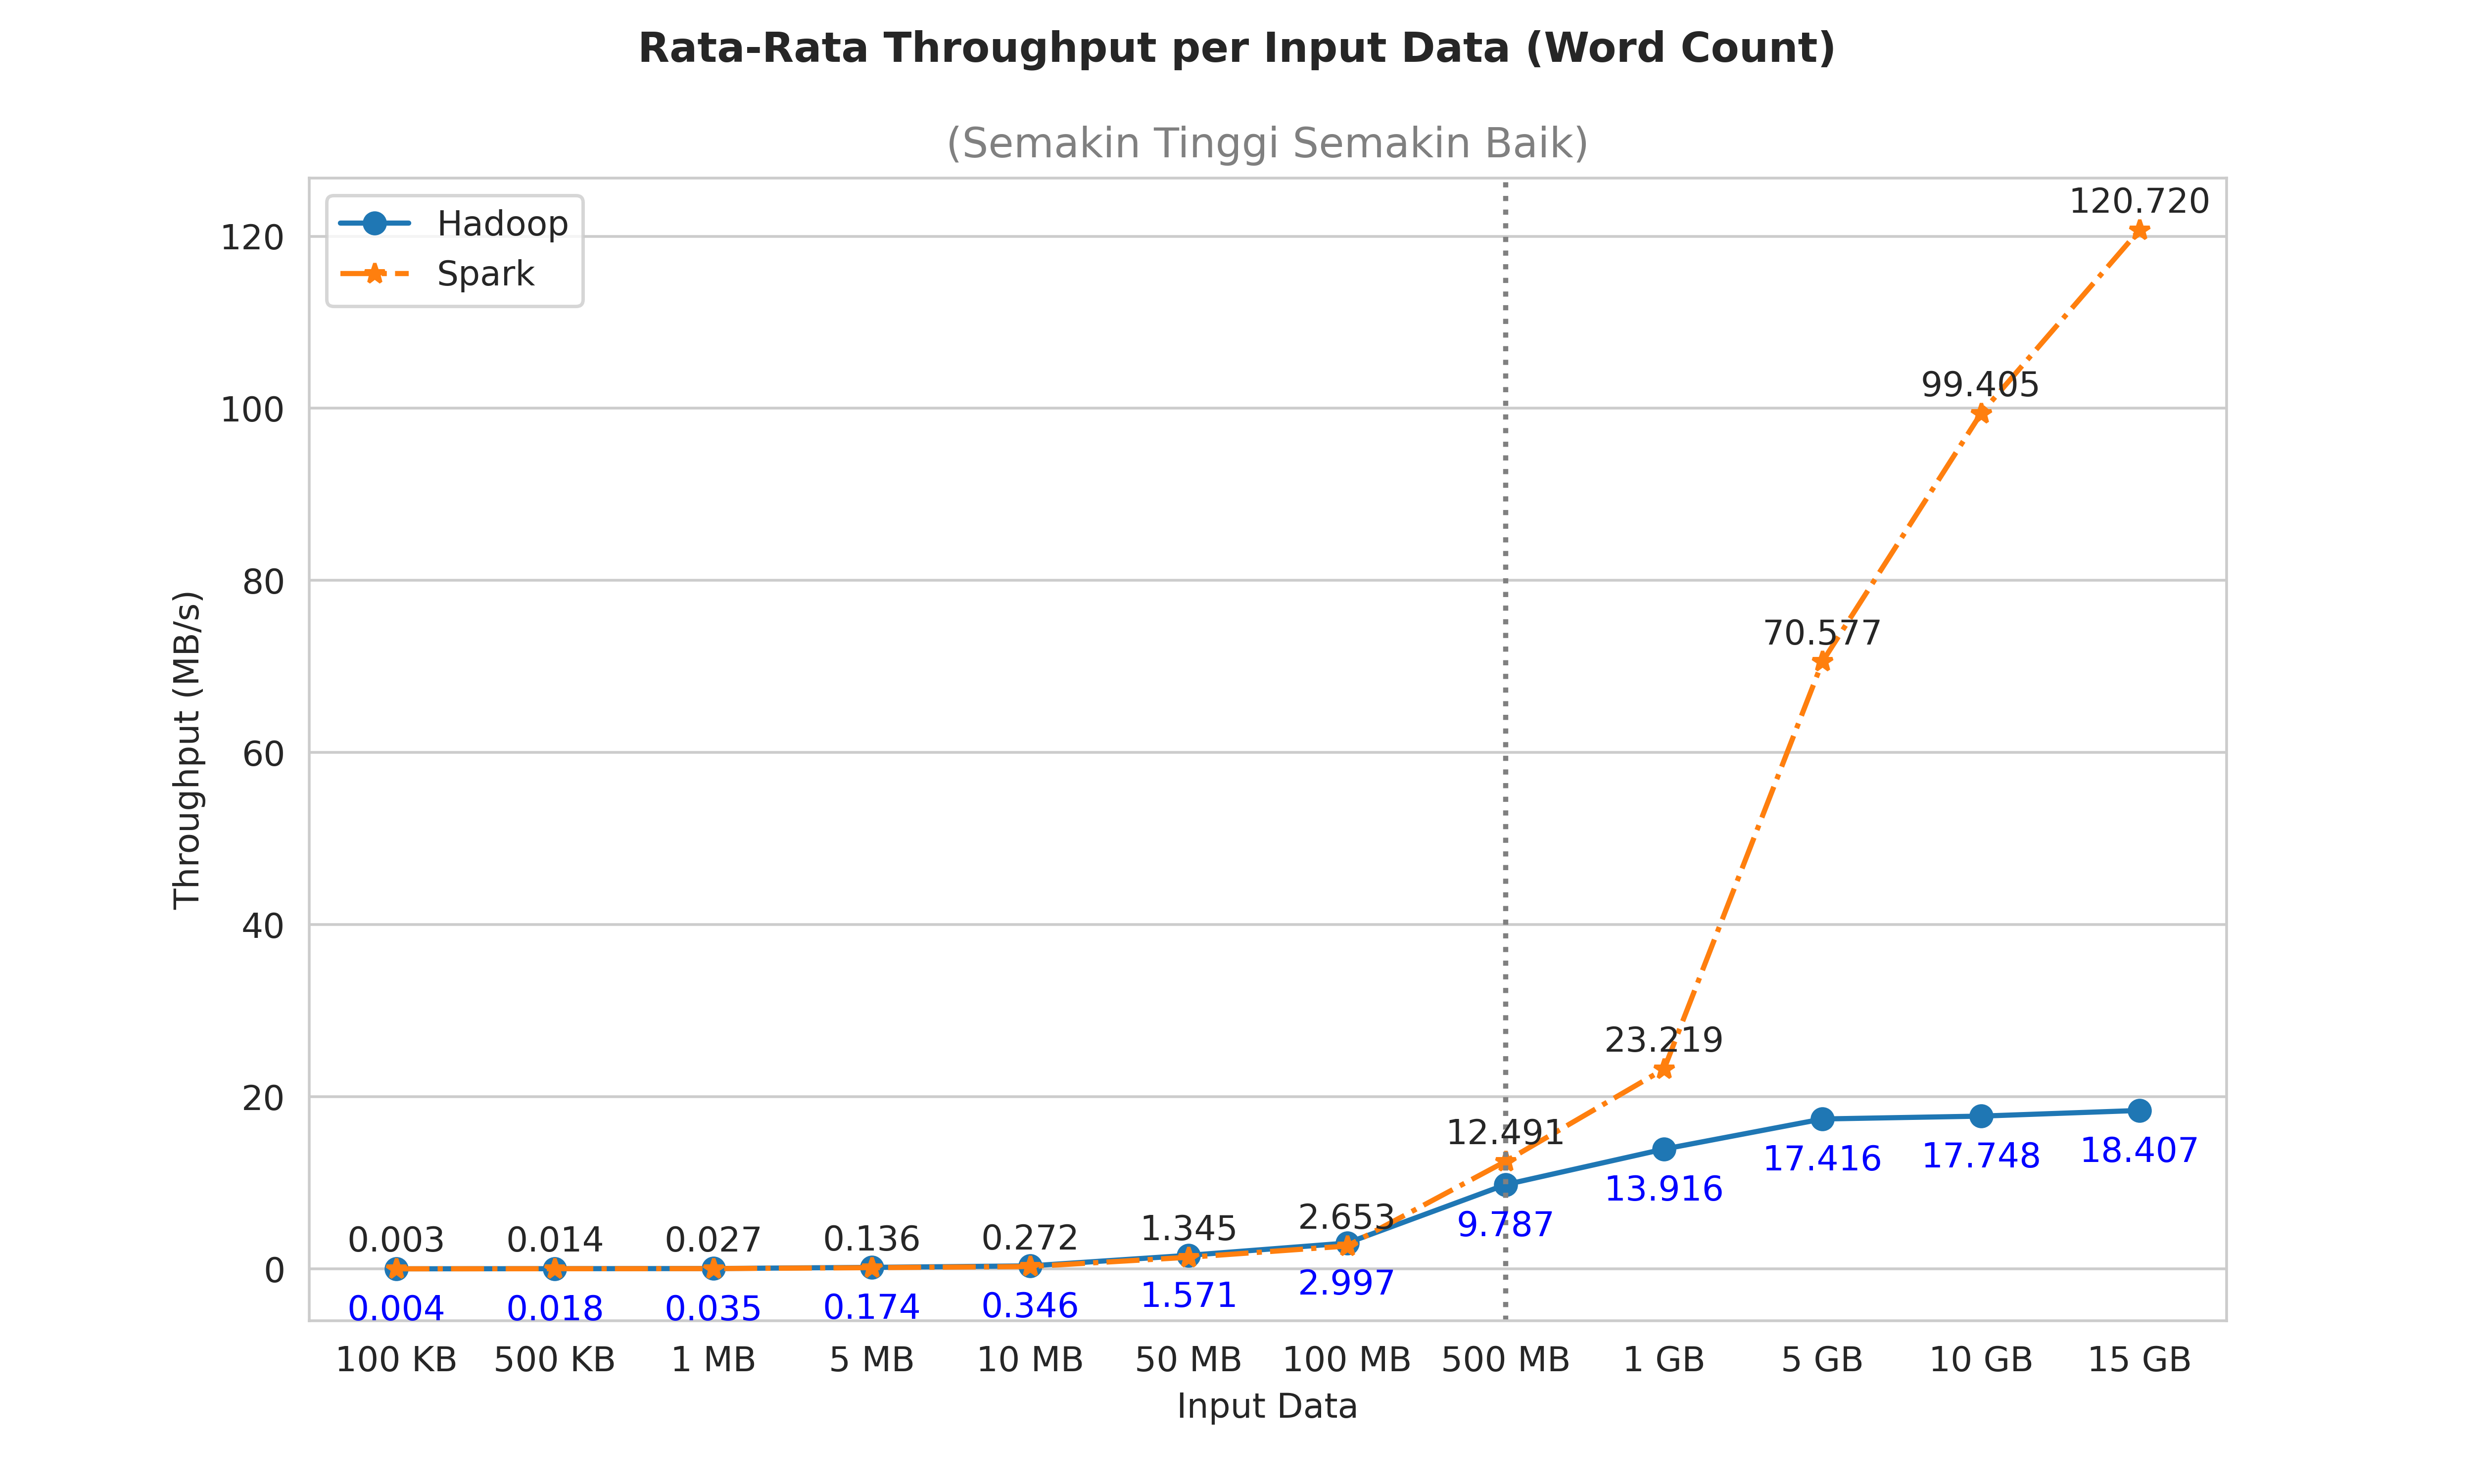
\includegraphics[width=0.95\textwidth]{figures/ch04/2-mean-throughput-wordcount.png}
    \caption{Rata-rata \textit{Throughput (Word Count)}}
    \label{fig:mean-throughput-wordcount}
\end{figure}

Pada beban kerja \textit{word count}, Spark juga mengungguli Hadoop dalam hal \textit{throughput} dengan perbedaan yang lebih besar daripada beban kerja \textit{sort}. Awalnya, \textit{throughput} Spark dan Hadoop sama dan saling berhimpit sejak input data 100 KB-100 MB. Spark mulai menunjukkan \textit{throughput} yang lebih tinggi pada ukuran data 500 MB. Pada ukuran data 15 GB, Spark mencapai throughput 120.72 MB/s, sedangkan Hadoop hanya mencapai 18.41 MB/s.

Rata-rata \textit{throughput} ini menunjukkan bahwa Spark lebih unggul dalam menangani data berukuran besar untuk kedua tugas pemrosesan data tersebut. Spark mampu mempertahankan throughput yang lebih tinggi dibandingkan Hadoop, terutama saat menangani data berukuran besar, dengan rincian sebagai berikut:
\begin{enumerate}
\item Untuk beban kerja \textit{sort}, Hadoop lebih unggul pada ukuran data di bawah 1 GB, sedangkan Spark mulai unggul pada ukuran data 1 GB dan seterusnya.
\item Untuk beban kerja \textit{word count}, Spark lebih unggul pada ukuran data 500 MB hingga 15 GB.
\end{enumerate}

Secara keseluruhan, Spark menunjukkan kinerja yang lebih baik dalam hal throughput terutama pada data berukuran besar, sementara Hadoop masih menunjukkan performa yang kompetitif pada data berukuran kecil hingga menengah.


%% --------------------------
\newpage
\subsection{Laju Perubahan (\textit{Rate of Change})}

Laju perubahan (ROC) menggambarkan kecepatan perubahan suatu variabel dalam periode waktu tertentu. ROC diwakili oleh kemiringan garis dan sering diilustrasikan dengan huruf delta ($\Delta$). Dalam konteks evaluasi performa sistem seperti Hadoop dan Spark, ROC dapat diaplikasikan untuk menganalisis:
\begin{enumerate}
	\item \textit{\textbf{Execution Time}}. ROC dari \textit{execution time} menunjukkan seberapa cepat waktu eksekusi tugas berubah seiring dengan peningkatan beban kerja (misalnya, jumlah data yang diproses). Nilai ROC positif mengindikasikan peningkatan performa, sementara nilai negatif mengindikasikan penurunan performa. Artinya, sistem membutuhkan waktu lebih lama untuk memproses data seiring bertambahnya beban, mengindikasikan potensi bottleneck atau masalah skalabilitas.
	\item \textit{\textbf{Throughput}}: ROC dari \textit{throughput} menunjukkan seberapa cepat laju pemrosesan data berubah seiring dengan peningkatan beban kerja. Nilai ROC positif mengindikasikan peningkatan performa, sementara nilai negatif mengindikasikan penurunan performa.\\
\end{enumerate}


\textbf{Laju Perubahan Waktu Eksekusi terhadap Input Data (\textit{Sort})}

Gambar \ref{fig:3-0-dur-sort} menunjukkan laju perubahan waktu eksekusi Hadoop-Spark terhadap input data pada beban kerja \textit{sort}. Hasil dan analisis dari gambar ini dapat dijelaskan sebagai berikut:
\begin{enumerate}
\item \textbf{100 KB - 10 MB:}
\begin{itemize}
\item \textit{Spark:} Laju perubahan (ROC) pada data input 500 KB sampai 5 MB cenderung naik, dimulai dari nilai ROC pada 500 KB sebesar -5.4 $\times 10^{-9}$ hingga mencapai 6.7 $\times 10^{-8}$ pada 5 MB. Namun, pada input data 10 MB, laju mengalami penurunan menjadi -8.4 $\times 10^{-9}$.
\item \textit{Hadoop:} ROC menunjukkan fluktuasi yang cukup signifikan. Pada 500 KB, nilai ROC adalah -1.1 $\times 10^{-6}$, kemudian naik drastis pada 5 MB menjadi 3.9 $\times 10^{-6}$ sebelum turun kembali pada 10 MB menjadi -9.7 $\times 10^{-9}$.
\end{itemize}
\item \textbf{10 MB - 1 GB:}
\begin{itemize}
    \item \textit{Spark:} Laju perubahan mengalami peningkatan dari 10 MB ke 50 MB (1.7 $\times 10^{-8}$), kemudian sedikit menurun secara bertahap hingga 1 GB (6.7 $\times 10^{-9}$).
    \item \textit{Hadoop:} Pada rentang ini, nilai ROC mengalami penurunan secara bertahap dari 50 MB ke 1 GB, dimulai dari nilai ROC sebesar 2.1 $\times 10^{-6}$ pada 50 MB hingga mencapai 1.1 $\times 10^{-8}$ pada 1 GB.
\end{itemize}
\item \textbf{1 GB - 15 GB:}
\begin{itemize}
    \item \textit{Spark:} Pada rentang ini, nilai ROC mulai dari 1 GB hingga 5 GB menunjukkan peningkatan yang signifikan, dari 6.7 $\times 10^{-9}$ menjadi 1.1 $\times 10^{-8}$. Selanjutnya, pada input data tertinggi, yaitu 15 GB, nilai ROC mengalami sedikit penurunan.
    \item \textit{Hadoop:} Nilai ROC pada input data 1 GB hingga 5 GB mengalami peningkatan yang drastis, mulai dari 1.1 $\times 10^{-8}$ menjadi 1.9 $\times 10^{-8}$. Peningkatan ini berlanjut hingga 15 GB dengan nilai ROC mencapai 2.5 $\times 10^{-8}$.
\end{itemize}
\end{enumerate}

Analisis menunjukkan bahwa baik Spark maupun Hadoop menunjukkan tren laju perubahan yang bervariasi tergantung pada ukuran input data. Spark cenderung memiliki fluktuasi yang lebih halus, sedangkan Hadoop menunjukkan perubahan yang lebih drastis terutama pada ukuran input data yang lebih kecil.\\

\textbf{Laju Perubahan Waktu Eksekusi terhadap Input Data (\textit{Word Count})}

Gambar \ref{fig:3-0-dur-wc} menunjukkan laju perubahan waktu eksekusi Hadoop-Spark terhadap input data pada beban kerja \textit{word count}. Hasil dan analisis dari gambar ini dapat dijelaskan sebagai berikut:

\begin{enumerate}
\item \textbf{100 KB - 10 MB:}
\begin{itemize}
\item \textit{Spark:} Laju perubahan (ROC) pada data input 500 KB mencapai puncaknya sebesar 5.4 $\times 10^{-7}$, tetapi menurun drastis pada 1 MB menjadi 2.1 $\times 10^{-8}$. Pada input data 5 MB dan 10 MB, laju perubahan terus menurun hingga mencapai -9.3 $\times 10^{-9}$.
\item \textit{Hadoop:} ROC juga menunjukkan fluktuasi yang signifikan dengan puncak pada 1 MB sebesar 1.9 $\times 10^{-6}$. Setelah itu, ROC menurun pada 5 MB menjadi -9.3 $\times 10^{-8}$ dan lebih lanjut pada 10 MB mencapai 1.1 $\times 10^{-8}$.
\end{itemize}

\item \textbf{10 MB - 1 GB:}
\begin{itemize}
    \item \textit{Spark:} Laju perubahan mengalami peningkatan dari 10 MB ke 50 MB (1.1 $\times 10^{-8}$) sebelum sedikit menurun pada 100 MB (-9.7 $\times 10^{-9}$). Selanjutnya, ROC menunjukkan fluktuasi kecil pada 500 MB (5.6 $\times 10^{-9}$) hingga 1 GB (5.8 $\times 10^{-9}$).
    \item \textit{Hadoop:} Pada rentang ini, nilai ROC menunjukkan fluktuasi dengan puncak pada 50 MB (7.0 $\times 10^{-8}$) dan penurunan pada 100 MB (2.9 $\times 10^{-8}$). Setelah itu, ROC stabil dari 500 MB (4.2 $\times 10^{-8}$) hingga 1 GB (4.0 $\times 10^{-8}$).
\end{itemize}

\item \textbf{1 GB - 15 GB:}
\begin{itemize}
    \item \textit{Spark:} Pada rentang ini, nilai ROC mulai dari 1 GB hingga 5 GB menunjukkan peningkatan yang signifikan, dari 5.8 $\times 10^{-9}$ menjadi 6.6 $\times 10^{-9}$. Namun, pada input data tertinggi, yaitu 15 GB, nilai ROC mengalami sedikit penurunan menjadi 4.5 $\times 10^{-9}$.
    \item \textit{Hadoop:} Nilai ROC pada input data 1 GB hingga 5 GB mengalami peningkatan yang drastis, mulai dari 4.0 $\times 10^{-8}$ menjadi 5.1 $\times 10^{-8}$. Peningkatan ini berlanjut hingga 10 GB dengan nilai ROC mencapai 5.3 $\times 10^{-8}$, sebelum menurun pada 15 GB menjadi 4.8 $\times 10^{-8}$.\\
\end{itemize}
\end{enumerate}

\textbf{Laju Perubahan \textit{Throughput} terhadap Input Data (\textit{Sort})}

Gambar \ref{fig:3-0-th-sort} menunjukkan laju perubahan \textit{throughput} Hadoop-Spark terhadap input data pada beban kerja \textit{sort}. Hasil dan analisis dari gambar ini dapat dijelaskan sebagai berikut:

\begin{enumerate}
\item \textbf{100 KB - 10 MB:}
\begin{itemize}
\item \textit{Spark:} Laju perubahan \textit{throughput} pada data input 500 KB mencapai puncaknya sebesar 2.8 $\times 10^{-2}$. Pada input data 5 MB dan 10 MB, laju perubahan \textit{throughput} tetap stabil pada 2.8 $\times 10^{-2}$.
\item \textit{Hadoop:} Laju perubahan \textit{throughput} pada data input 500 KB mencapai puncaknya sebesar 3.8 $\times 10^{-2}$. Pada input data 5 MB dan 10 MB, laju perubahan \textit{throughput} tetap stabil pada 3.8 $\times 10^{-2}$.
\end{itemize}
\item \textbf{10 MB - 1 GB:}
\begin{itemize}
    \item \textit{Spark:} Laju perubahan \textit{throughput} pada data input 10 MB mencapai 2.8 $\times 10^{-2}$. Setelah itu, laju perubahan \textit{throughput} menurun secara bertahap dari 50 MB hingga 1 GB, mencapai nilai 2.1 $\times 10^{-2}$.
    \item \textit{Hadoop:} Pada rentang ini, laju perubahan \textit{throughput} menunjukkan penurunan yang lebih tajam dari 10 MB (3.8 $\times 10^{-2}$) hingga 1 GB (2.2 $\times 10^{-2}$), dengan penurunan terbesar terjadi pada 500 MB (3.1 $\times 10^{-2}$).
\end{itemize}

\item \textbf{1 GB - 15 GB:}
\begin{itemize}
    \item \textit{Spark:} Laju perubahan \textit{throughput} pada rentang ini mengalami penurunan secara bertahap dari 1 GB (2.1 $\times 10^{-2}$) hingga 15 GB (8.8 $\times 10^{-4}$). Penurunan terbesar terjadi antara 5 GB (8.2 $\times 10^{-3}$) dan 10 GB (2.9 $\times 10^{-3}$).
    \item \textit{Hadoop:} Laju perubahan \textit{throughput} pada rentang ini juga mengalami penurunan yang signifikan dari 1 GB (2.2 $\times 10^{-2}$) hingga 15 GB (2.5 $\times 10^{-4}$). Penurunan terbesar terjadi antara 5 GB (3.9 $\times 10^{-3}$) dan 10 GB (2.1 $\times 10^{-4}$).
\end{itemize}
\end{enumerate}

Analisis menunjukkan bahwa baik Spark maupun Hadoop menunjukkan tren penurunan laju perubahan \textit{throughput} seiring dengan peningkatan ukuran input data. Spark cenderung memiliki laju perubahan \textit{throughput} yang lebih stabil pada ukuran input data kecil, sedangkan Hadoop menunjukkan penurunan yang lebih tajam terutama pada ukuran input data yang lebih besar.\\

\textbf{Laju Perubahan \textit{Throughput} terhadap Input Data (\textit{Word Count})}

Gambar \ref{fig:3-0-th-wc} menunjukkan laju perubahan \textit{throughput} Hadoop dan Spark terhadap input data pada beban kerja \textit{word count}. Hasil dan analisis dari gambar ini dapat dijelaskan sebagai berikut:

\begin{enumerate}
\item \textbf{100 KB - 10 MB:}
\begin{itemize}
\item \textit{Spark:} Laju perubahan \textit{throughput} pada data input 500 KB mencapai puncaknya sebesar 2.8 $\times 10^{-2}$. Pada input data 5 MB dan 10 MB, laju perubahan \textit{throughput} tetap stabil pada 2.8 $\times 10^{-2}$.
\item \textit{Hadoop:} Laju perubahan \textit{throughput} pada data input 500 KB mencapai puncaknya sebesar 3.7 $\times 10^{-2}$. Pada input data 5 MB, laju perubahan \textit{throughput} sedikit menurun menjadi 3.5 $\times 10^{-2}$ dan tetap stabil pada input data 10 MB.
\end{itemize}
\item \textbf{10 MB - 1 GB:}
\begin{itemize}
\item \textit{Spark:} Laju perubahan \textit{throughput} pada data input 10 MB mencapai 2.8 $\times 10^{-2}$. Setelah itu, laju perubahan \textit{throughput} menurun secara bertahap dari 50 MB hingga 1 GB, mencapai nilai 2.2 $\times 10^{-2}$.
\item \textit{Hadoop:} Pada rentang ini, laju perubahan \textit{throughput} menunjukkan penurunan yang lebih tajam dari 10 MB (3.5 $\times 10^{-2}$) hingga 1 GB (8.4 $\times 10^{-3}$), dengan penurunan terbesar terjadi pada 500 MB (1.7 $\times 10^{-2}$).
\end{itemize}

\item \textbf{1 GB - 15 GB:}
\begin{itemize}
\item \textit{Spark:} Laju perubahan \textit{throughput} pada rentang ini mengalami penurunan secara bertahap dari 1 GB (2.2 $\times 10^{-2}$) hingga 15 GB (4.4 $\times 10^{-3}$). Penurunan terbesar terjadi antara 5 GB (1.2 $\times 10^{-2}$) dan 10 GB (5.9 $\times 10^{-3}$).
\item \textit{Hadoop:} Laju perubahan \textit{throughput} pada rentang ini juga mengalami penurunan yang signifikan dari 1 GB (8.4 $\times 10^{-3}$) hingga 15 GB (1.3 $\times 10^{-4}$). Penurunan terbesar terjadi antara 5 GB (8.9 $\times 10^{-4}$) dan 10 GB (6.8 $\times 10^{-5}$).
\end{itemize}
\end{enumerate}

Analisis menunjukkan bahwa baik Spark maupun Hadoop menunjukkan tren penurunan laju perubahan \textit{throughput} seiring dengan peningkatan ukuran input data. Spark cenderung memiliki laju perubahan throughput yang lebih stabil pada ukuran input data kecil, sedangkan Hadoop menunjukkan penurunan yang lebih tajam terutama pada ukuran input data yang lebih besar.\\

\textbf{Laju Perubahan Waktu Eksekusi Hadoop-Spark terhadap Input Data}

Gambar \ref{fig:3-grup-hadoop-spark} menunjukkan laju perubahan waktu eksekusi Hadoop dan Spark terhadap input data pada beban kerja \textit{sort} dan \textit{word count}. Hasil dan analisis dari gambar ini dapat dijelaskan sebagai berikut:

\begin{enumerate}
\item \textbf{100 KB - 10 MB:}
\begin{itemize}
\item \textit{Sort (Spark):} Laju perubahan waktu eksekusi mencapai puncaknya pada 5 MB sebesar 5.3. Setelah itu, laju perubahan waktu eksekusi menurun drastis pada 10 MB menjadi -5.0.
\item \textit{Word Count (Hadoop):} Laju perubahan waktu eksekusi mengalami puncak pada 1 MB sebesar 9.8. Setelah itu, terjadi penurunan yang signifikan pada 500 KB menjadi -3.7 dan terus menurun hingga 10 MB menjadi 5.6 $\times 10^{-2}$.
\end{itemize}
\item \textbf{10 MB - 1 GB:}
\begin{itemize}
\item \textit{Sort (Spark):} Laju perubahan waktu eksekusi menunjukkan peningkatan signifikan dari 50 MB (-5.0 $\times 10^{-2}$) hingga 500 MB (3.2 $\times 10^9$), lalu meningkat lagi hingga 1 GB mencapai 5.5 $\times 10^9$.
\item \textit{Word Count (Hadoop):} Laju perubahan waktu eksekusi meningkat tajam dari 50 MB (1.0 $\times 10^9$) hingga 1 GB (2.0 $\times 10^1$).
\end{itemize}

\item \textbf{1 GB - 15 GB:}
\begin{itemize}
\item \textit{Sort (Spark):} Laju perubahan waktu eksekusi terus meningkat seiring dengan penambahan ukuran input data. Pada 5 GB, laju perubahan mencapai 8.0 $\times 10^1$, lalu meningkat signifikan pada 10 GB mencapai 1.2 $\times 10^2$ dan mencapai puncaknya pada 15 GB sebesar 1.3 $\times 10^2$.
\item \textit{Word Count (Hadoop):} Laju perubahan waktu eksekusi juga meningkat seiring dengan penambahan ukuran input data. Pada 5 GB, laju perubahan mencapai 2.1 $\times 10^2$, lalu meningkat signifikan pada 10 GB mencapai 2.7 $\times 10^2$ dan sedikit menurun pada 15 GB menjadi 2.5 $\times 10^2$.
\end{itemize}
\end{enumerate}

Analisis menunjukkan bahwa baik Spark maupun Hadoop mengalami peningkatan laju perubahan waktu eksekusi seiring dengan peningkatan ukuran input data. Spark menunjukkan peningkatan yang lebih stabil pada beban kerja \textit{sort}, sedangkan Hadoop menunjukkan peningkatan yang lebih fluktuatif pada beban kerja \textit{word count}. Penurunan drastis pada beberapa titik input data tertentu menunjukkan adanya inefisiensi atau bottleneck dalam pengolahan data pada ukuran tersebut.


\begin{landscape}
\begin{figure}[h]
    \centering
    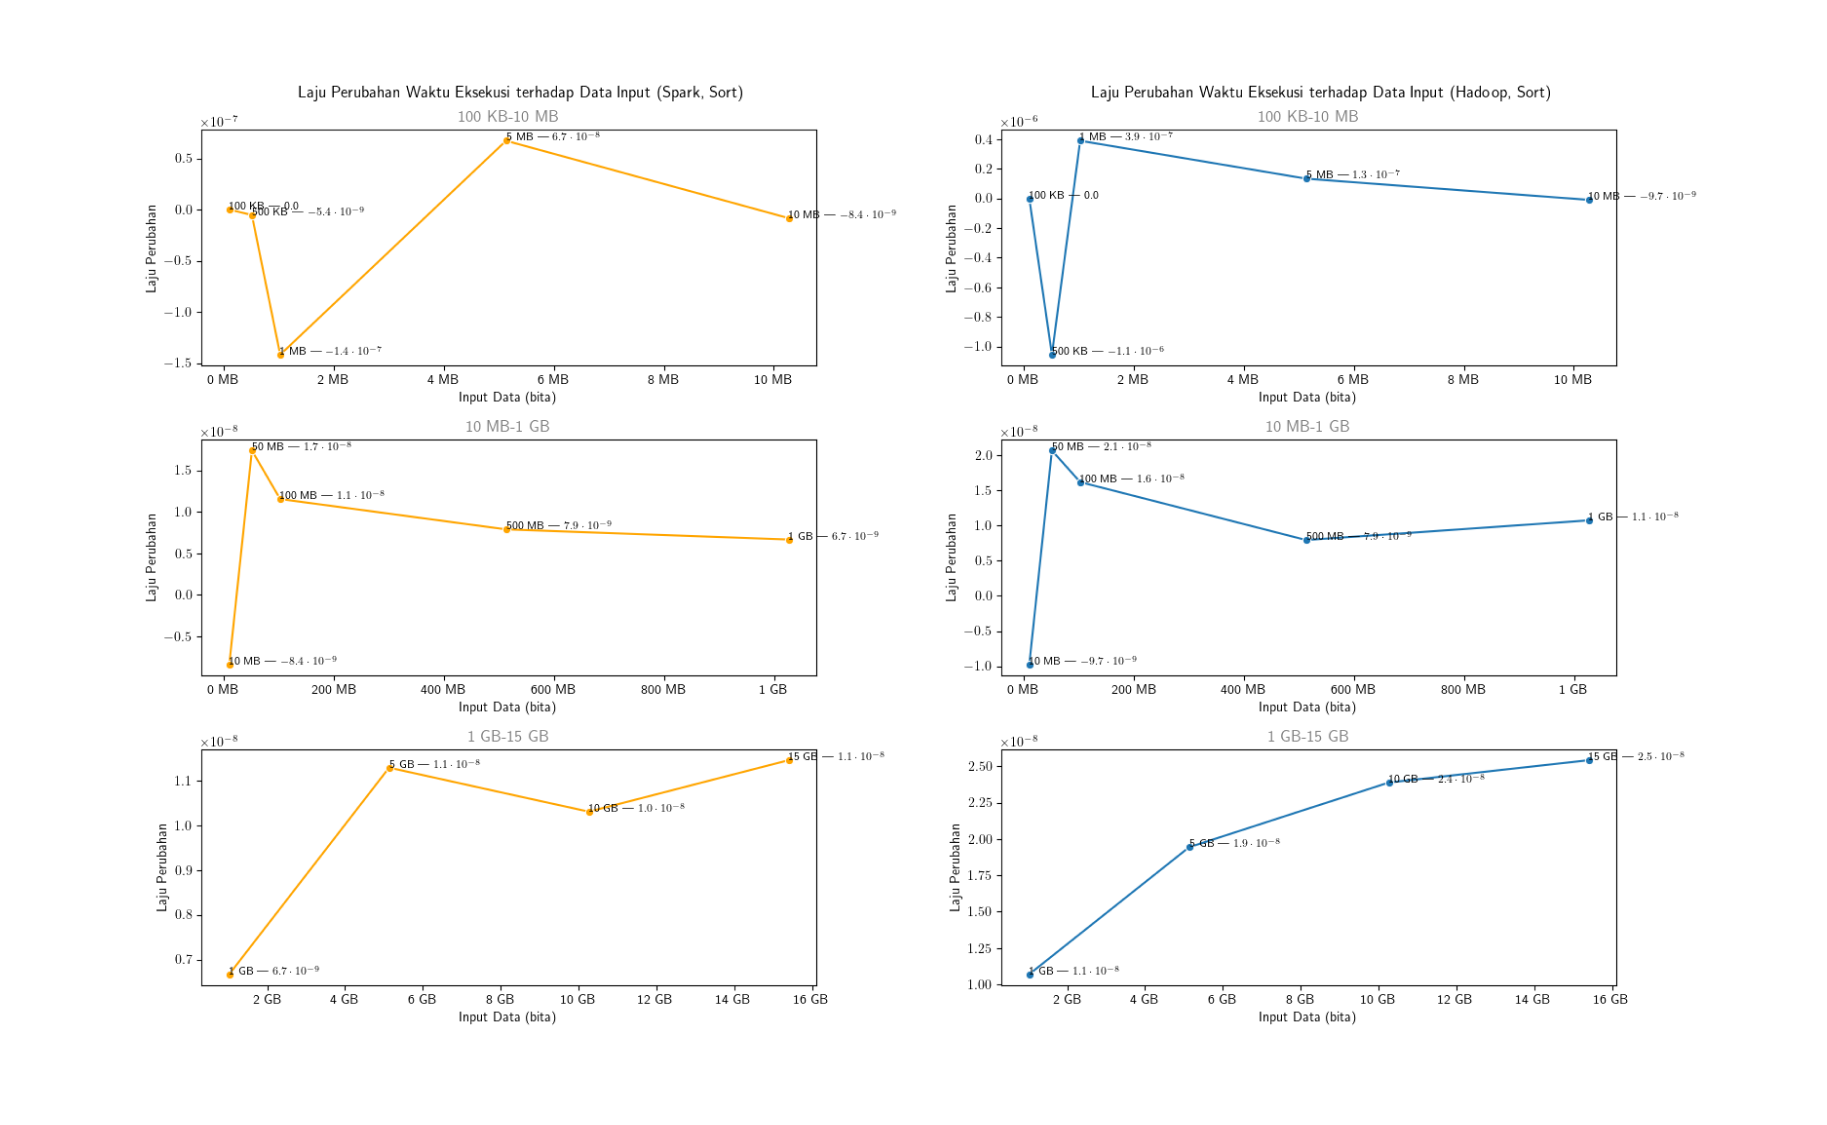
\includegraphics[height=0.6\linewidth]{figures/ch04/3-0-dur-sort.png}
    \caption{Laju Perubahan Waktu Eksekusi terhadap Input Data (\textit{Sort})}
    \label{fig:3-0-dur-sort}
\end{figure}
\end{landscape}

\begin{landscape}
\begin{figure}[h]
    \centering
    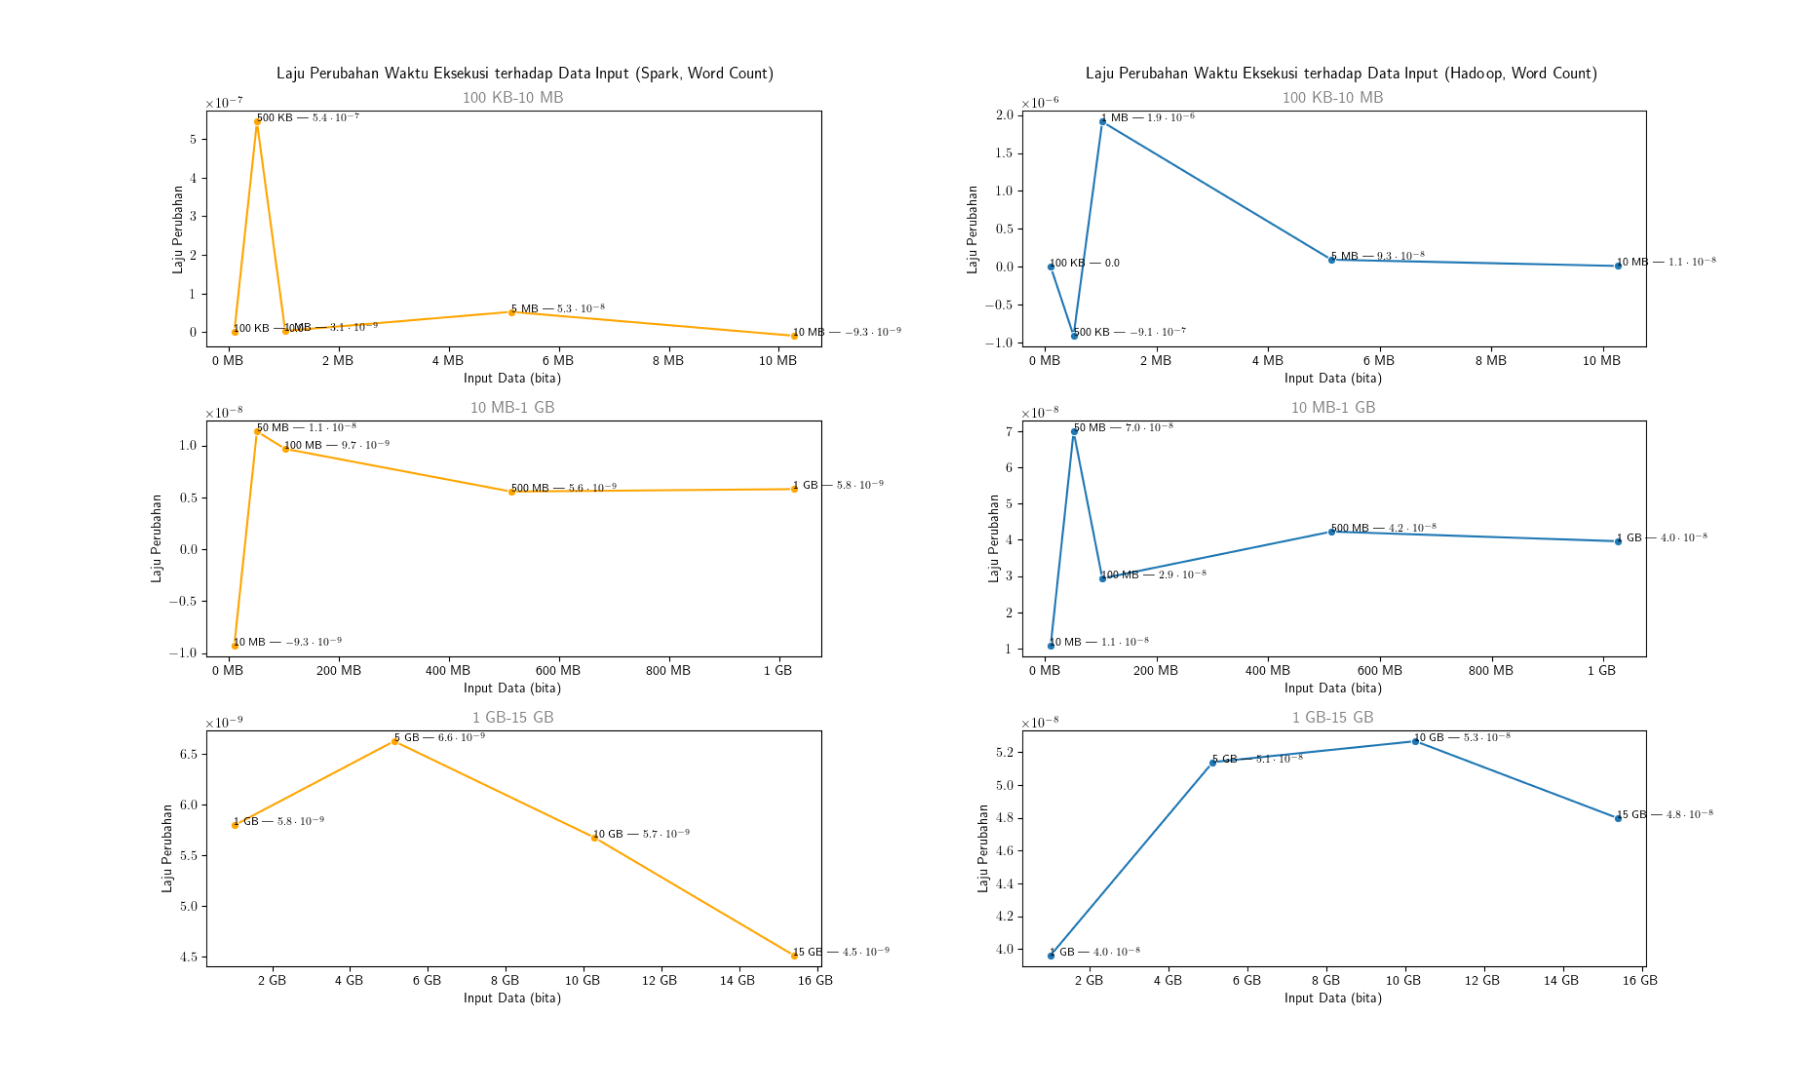
\includegraphics[height=0.6\linewidth]{figures/ch04/3-0-dur-wc.png}
    \caption{Laju Perubahan Waktu Eksekusi terhadap Input Data (\textit{Word Count})}
    \label{fig:3-0-dur-wc}
\end{figure}
\end{landscape}

\begin{landscape}
\begin{figure}[h]
    \centering
    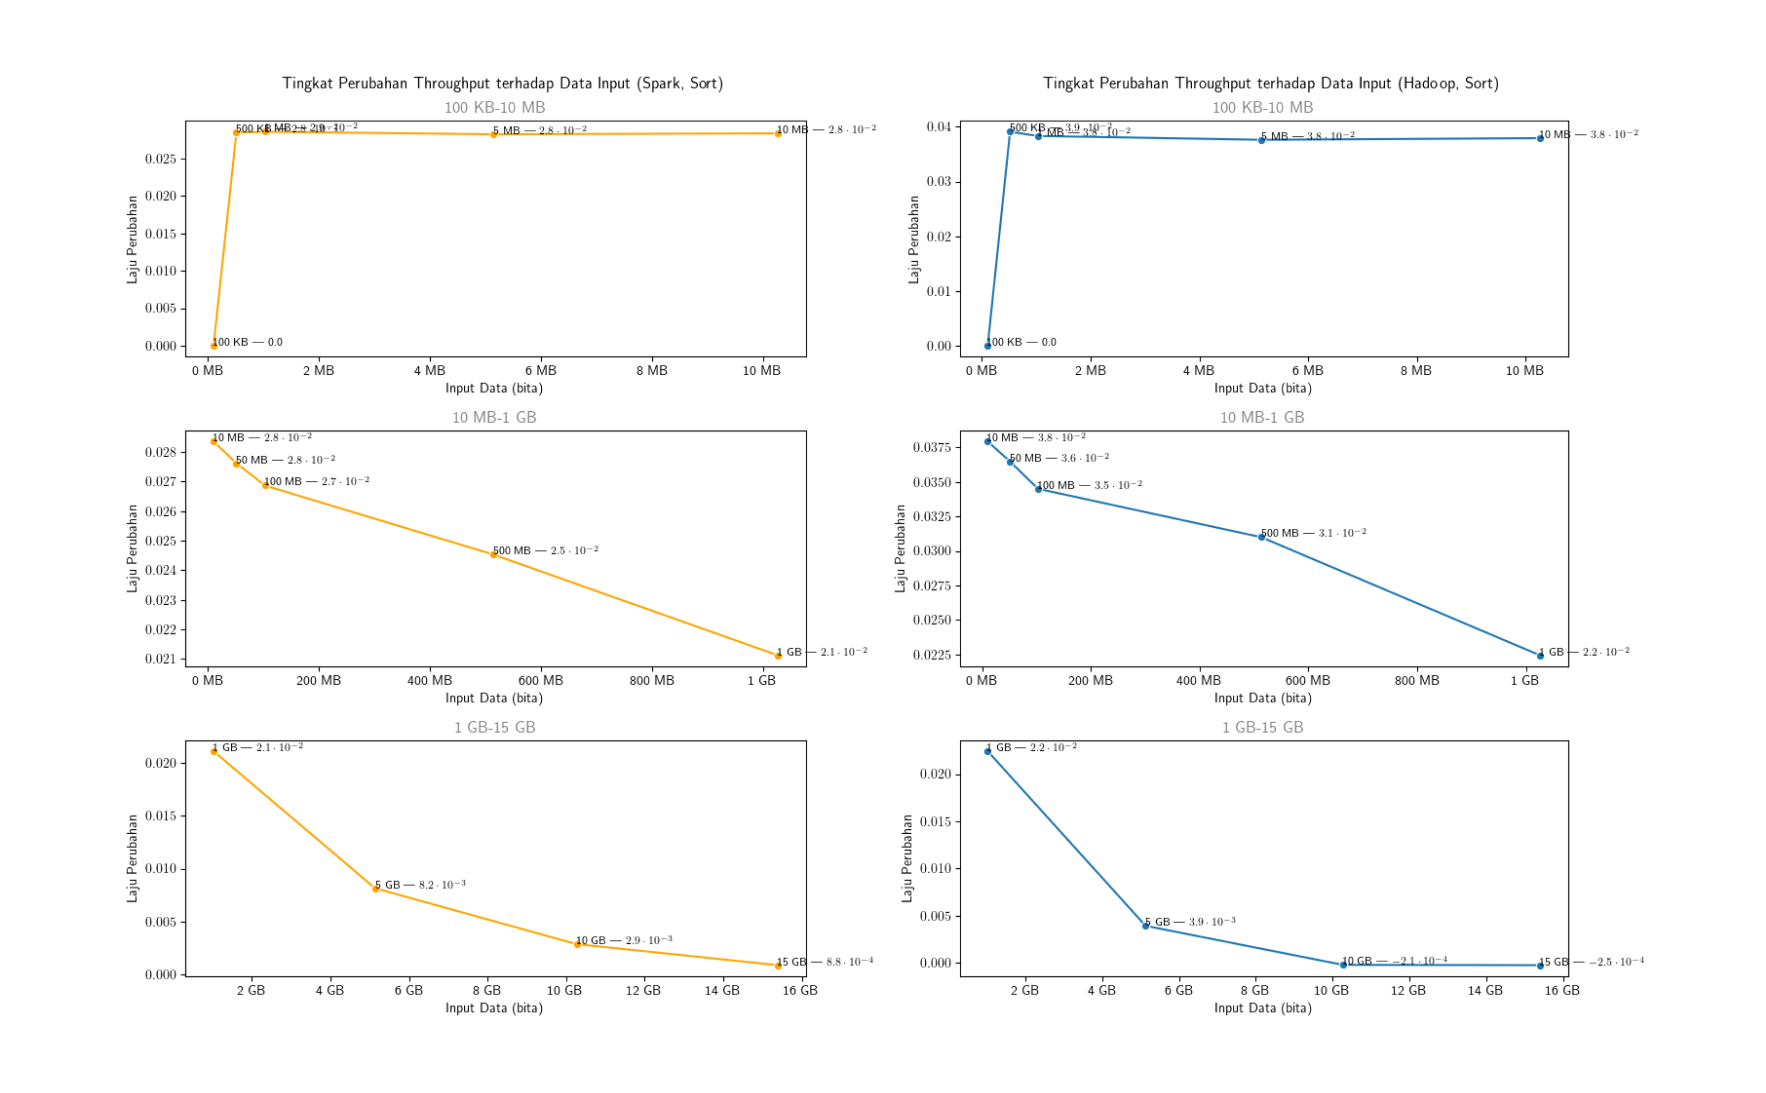
\includegraphics[height=0.6\linewidth]{figures/ch04/3-0-th-sort.png}
    \caption{Laju Perubahan \textit{Throughput} terhadap Input Data (\textit{Sort}}
    \label{fig:3-0-th-sort}
\end{figure}
\end{landscape}

\begin{landscape}
\begin{figure}[h]
    \centering
    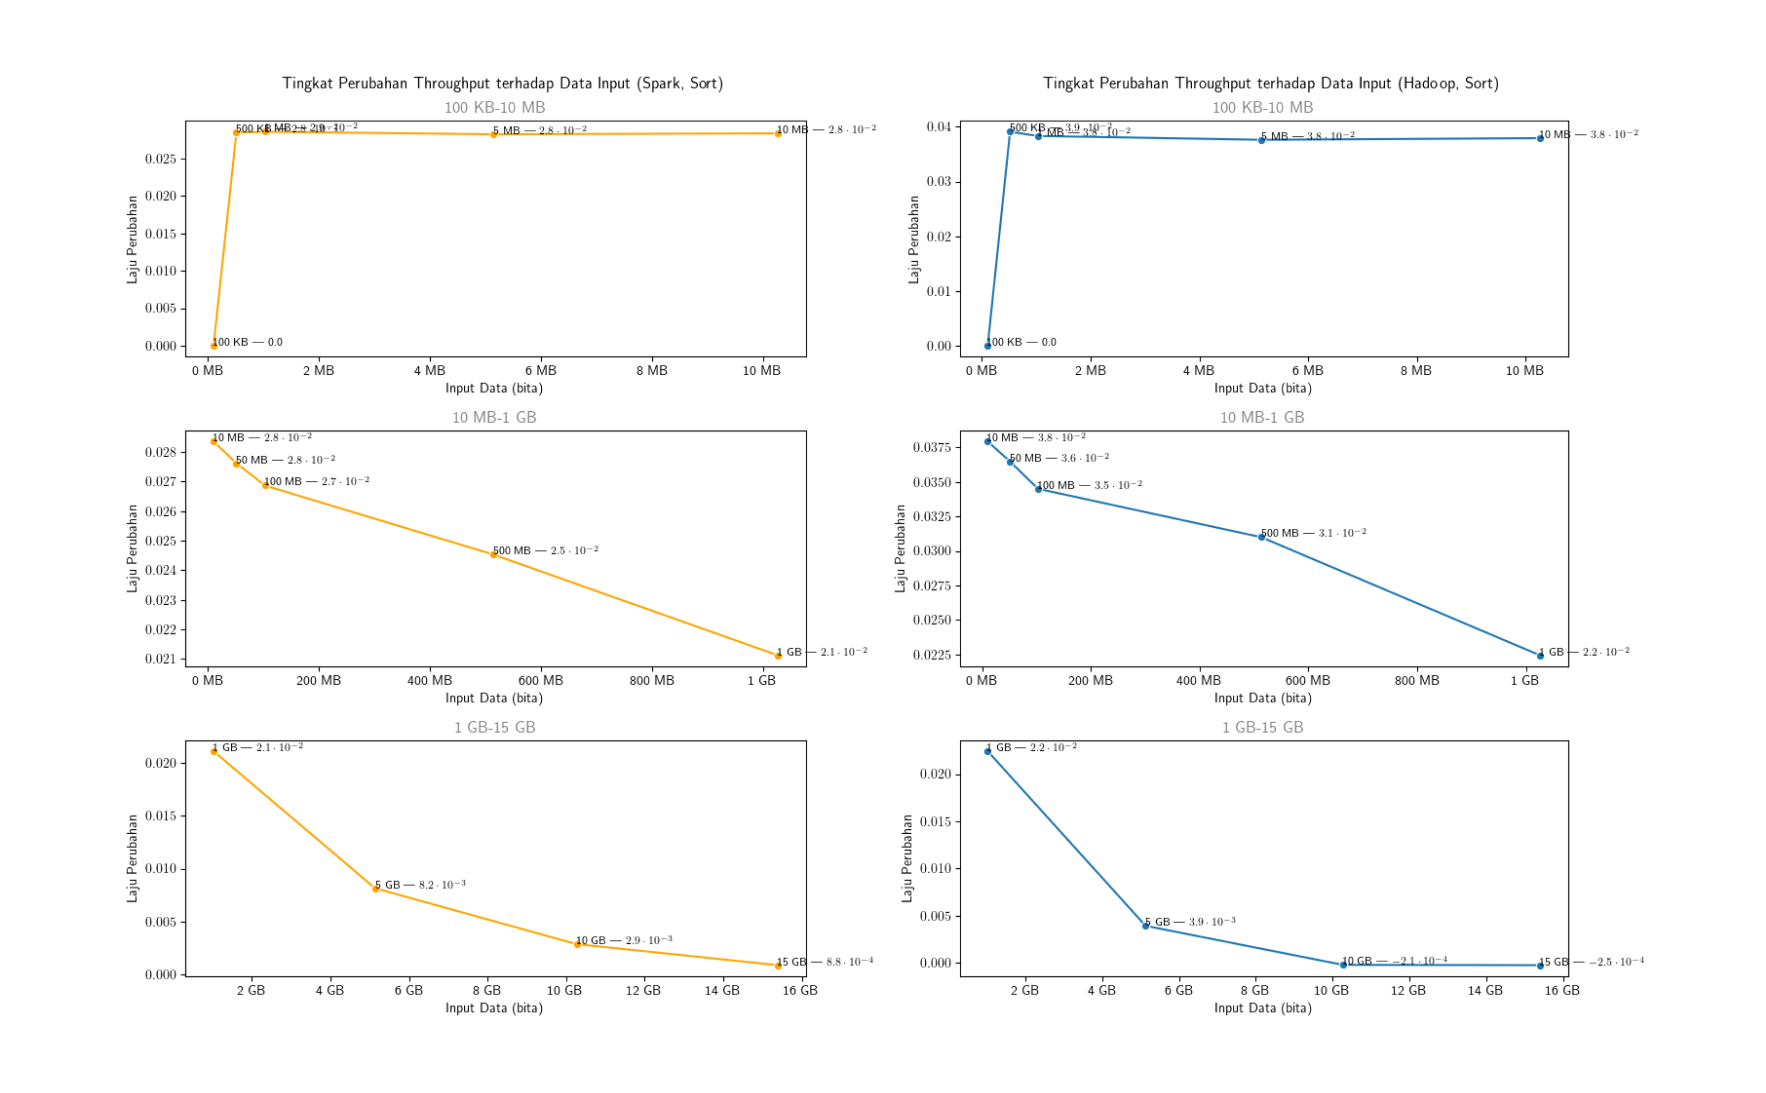
\includegraphics[height=0.6\linewidth]{figures/ch04/3-0-th-sort.png}
    \caption{Laju Perubahan \textit{Throughput} terhadap Input Data (\textit{Word Count}}
    \label{fig:3-0-th-wc}
\end{figure}
\end{landscape}

\begin{landscape}
\begin{figure}[h]
    \centering
    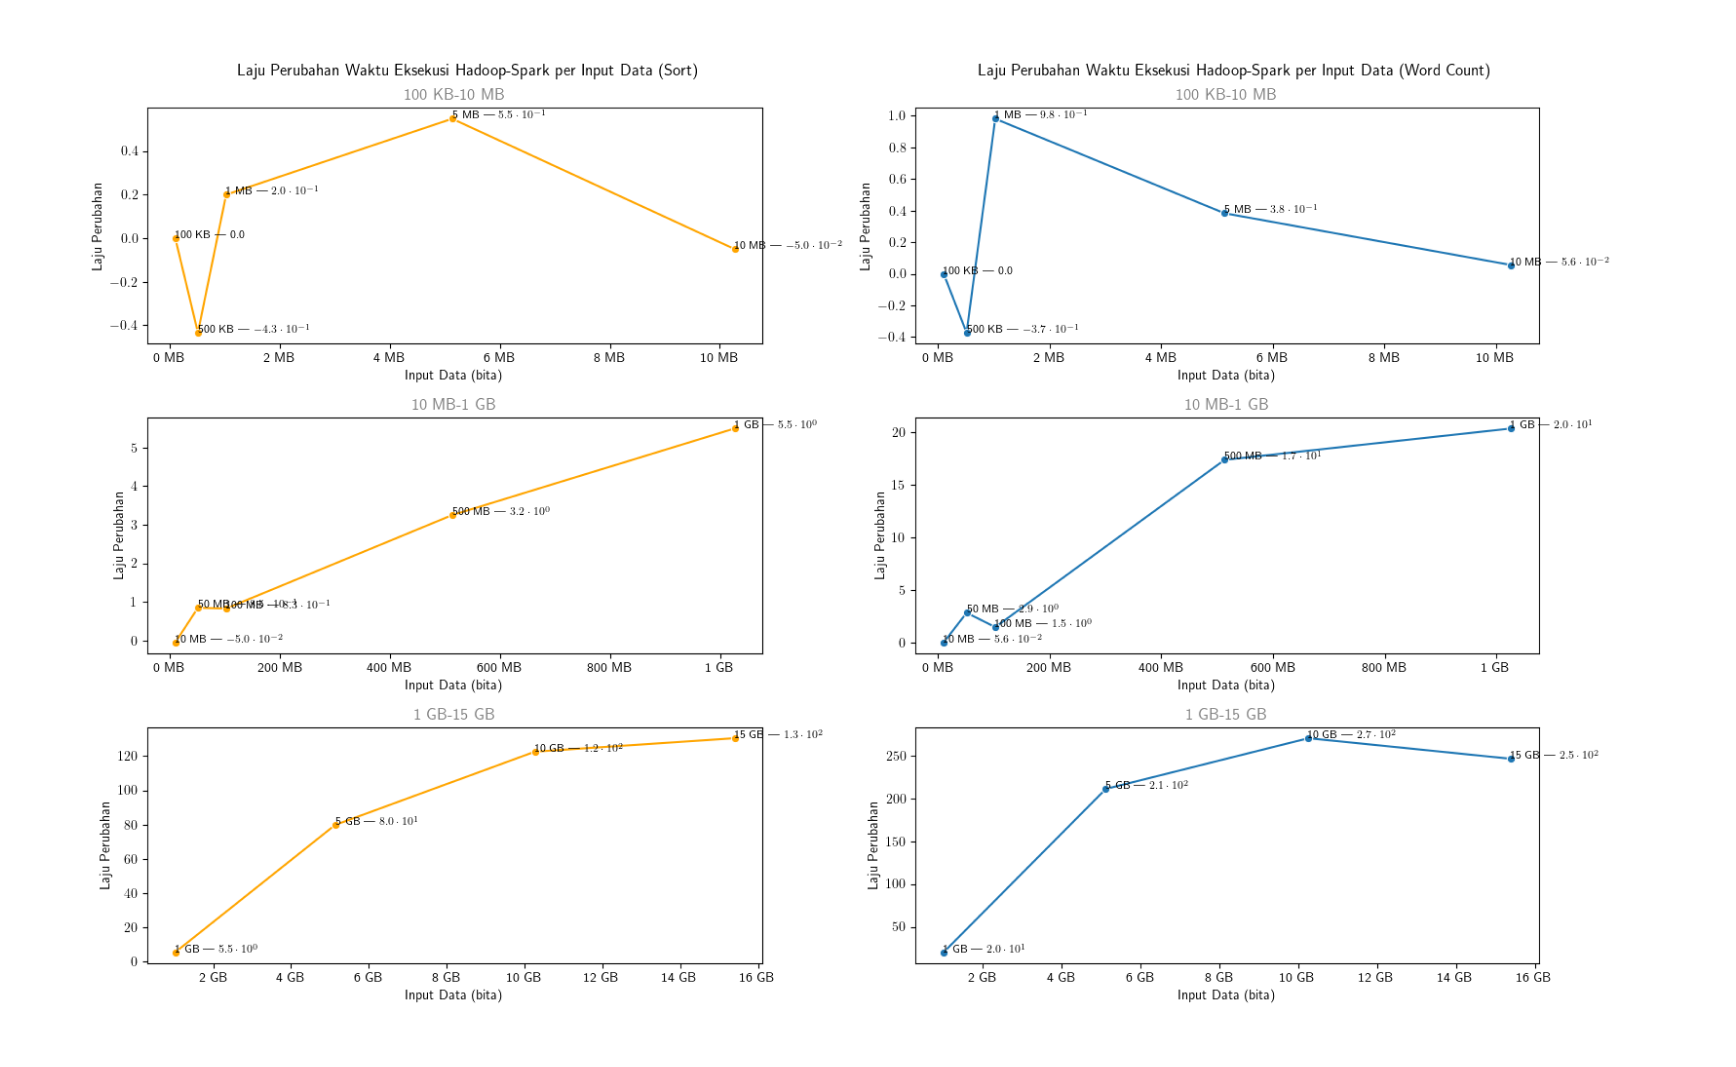
\includegraphics[height=0.6\linewidth]{figures/ch04/3-0-hadoop-spark}
    \caption{Laju Perubahan Waktu Eksekusi Hadoop-Spark terhadap Input Data}
    \label{fig:3-grup-hadoop-spark}
\end{figure}
\end{landscape}


% --------------------------------------

\newpage
\section{Analisis dan Evaluasi Hasil Eksperimen: Penggunaan Sumber Daya}
\subsection{Penggunaan CPU}
Gambar \ref{fig:4-penggunaan-cpu-all-sort} dan \ref{fig:4-penggunaan-cpu-all-wordcount} menunjukkan pola penggunaan CPU oleh Hadoop dan Spark untuk beban kerja \textit{sort} dan \textit{word count} pada berbagai ukuran data. Sumbu x mewakili waktu dalam detik, sedangkan sumbu y mewakili persentase penggunaan CPU. Setiap grafik menunjukkan ukuran data yang berbeda, mulai dari 100 KB hingga 15 GB. Titik hitam menandakan titik perpotongan Hadoop dan Spark.


Pada beban kerja \textit{sort} (Gambar \ref{fig:4-penggunaan-cpu-all-sort}), perbedaan pola penggunaan CPU antara Hadoop dan Spark semakin terlihat pada ukuran data yang lebih besar. Jika dilihat pada input data 100 KB-1 GB, penggunaan CPU pada masing-masing Hadoop dan Spark tidak berbeda jauh. Selanjutnya, pada input data 5 GB, 10 GB, dan 15 GB, penggunaan CPU Hadoop sangat fluktuatif berkisar pada 60\%-95\% pada dua per tiga bagian waktu awal eksekusi, dan pada satu per tiga waktu eksekusi mengalami penurunan yang berkisar pada 20\%-80\%. Berbeda dengan Hadoop, Spark memiliki penggunaan CPU yang lebih stabil (terkadang pada 60\%-80\%, dan terkadang pada 80\%-100\%).

Pada beban kerja \textit{word count} (Gambar \ref{fig:4-penggunaan-cpu-all-wordcount}), Hadoop menunjukkan penggunaan CPU yang lebih fluktuatif (naik turun) dan tinggi secara keseluruhan dibandingkan dengan Spark. Penggunaan CPU pada 10 detik pertama pada Hadoop berkisar pada 10\%-60\%. Setelah itu, penggunaan CPU-nya naik sampai ke 100\% dan naik turun. Jika dilihat dari input data yang lebih besar (15 GB), Hadoop memiliki pola CPU yang hampir sama pada setiap data input, yaitu 10 detik pertama berada pada 10\%-60\%, setengah pertama naik turun pada penggunaan CPU 60\%-100\%, dan setengah terakhir menurunkan penggunaan CPU pada 50\%-90\%. Selanjutnya, Spark juga memiliki pola tersendiri. Penggunaan CPU Spark pada detik pertama sampai detik ke 15 fluktuatif pada 20\%-50\%, hingga pada detik 16 sampai detik ke 35 turun ke 0\%, dan baru naik lagi pada detik ke 35. Hal yang menarik juga adalah penggunaan CPU Spark tidak menyentuh 100\%, tetapi memiliki waktu eksekusi beban kerja yang lebih cepat pada \textit{word count}.

Pada kedua tugas, terlihat bahwa beban kerja \textit{word count} cenderung menunjukkan pola penggunaan CPU yang lebih tinggi dan konsisten dibandingkan dengan beban kerja \textit{sort}. Pada beban kerja \textit{word count}, umumnya penggunaan CPU Hadoop lebih tinggi dan merata di sepanjang waktu eksekusi jika dibandingkan dengan Spark. Di sisi lain, beban kerja \textit{sort} menunjukkan penggunaan CPU yang cenderung lebih fluktuatif, dengan periode lonjakan dan penurunan yang signifikan, baik pada Hadoop maupun Spark.

Secara keseluruhan, Hadoop cenderung menggunakan CPU dengan lebih intensif dan fluktuatif dibandingkan Spark, terutama pada tugas \textit{word count}. Spark, meskipun tidak selalu menggunakan CPU hingga 100\%, mampu menyelesaikan tugas dengan waktu eksekusi yang lebih cepat, menunjukkan efisiensi penggunaan sumber daya yang lebih baik.

\begin{landscape}
\begin{figure}[h]
    \centering
    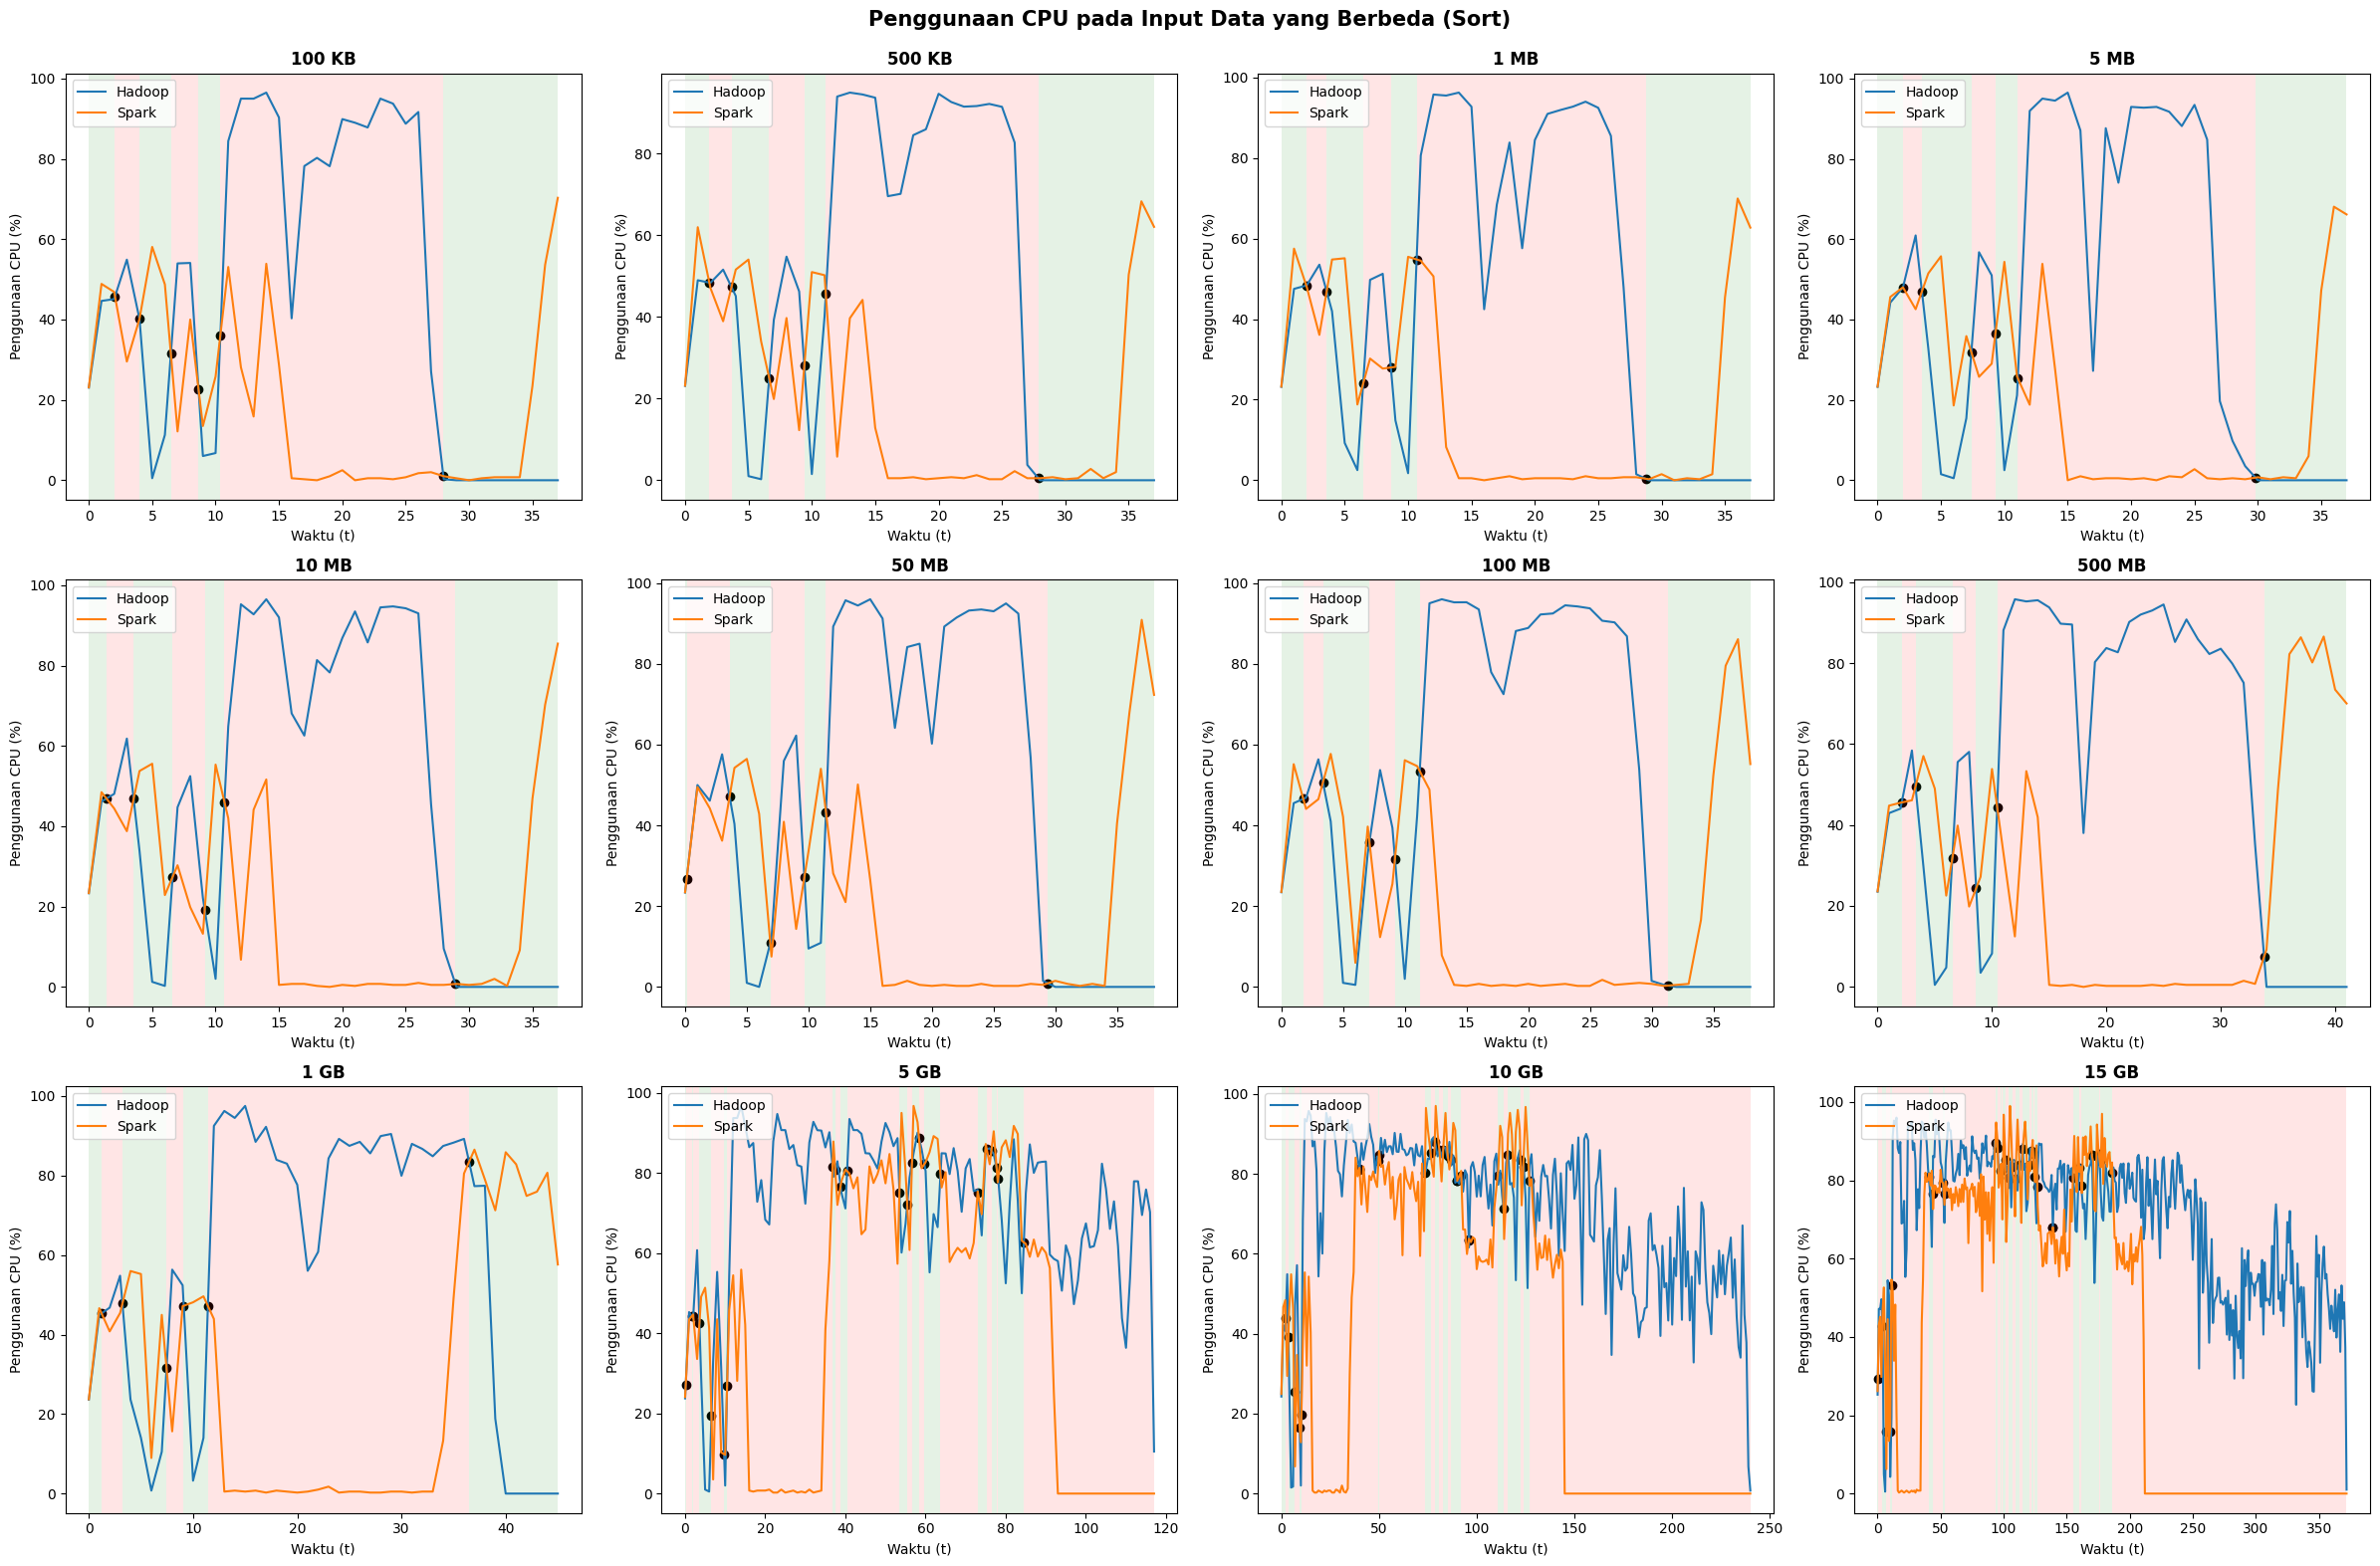
\includegraphics[height=0.6\linewidth]{figures/ch04/4-penggunaan-cpu-all-sort.png}
    \caption{Penggunaan CPU (\textit{Sort})}
    \label{fig:4-penggunaan-cpu-all-sort}
\end{figure}
\end{landscape}

\begin{landscape}
\begin{figure}[h]
    \centering
    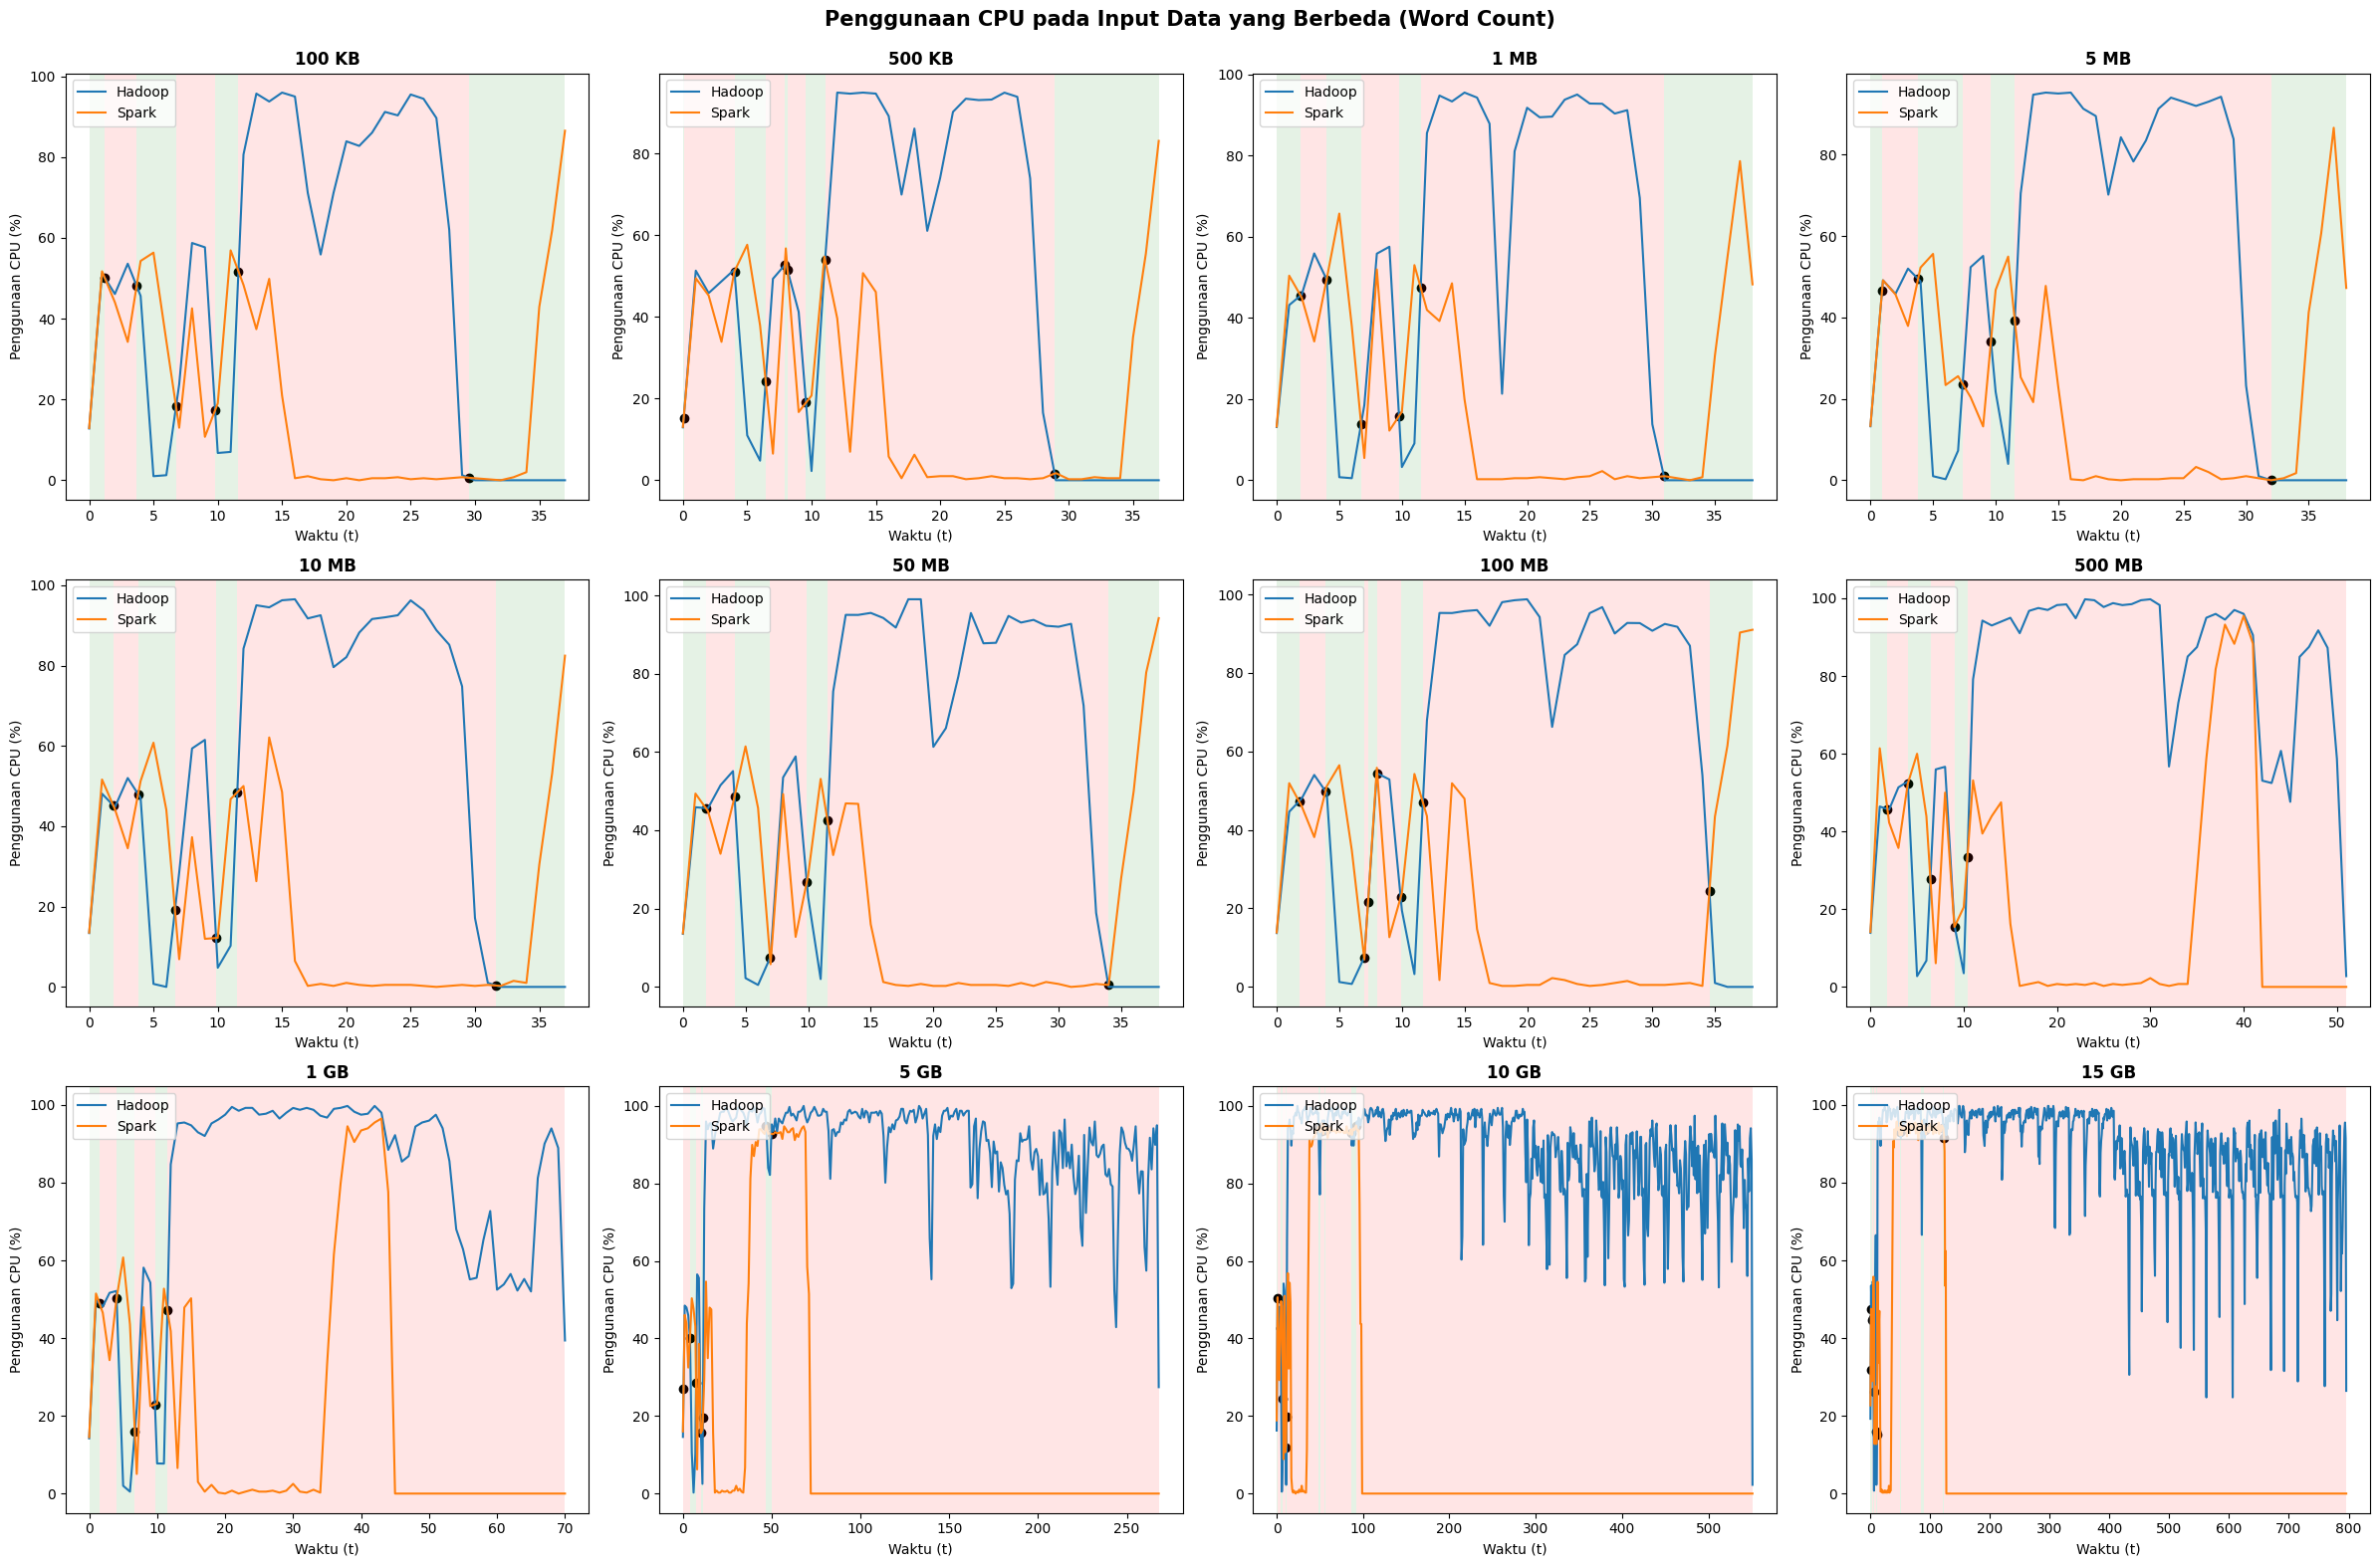
\includegraphics[height=0.6\linewidth]{figures/ch04/4-penggunaan-cpu-all-wordcount.png}
    \caption{Penggunaan CPU (\textit{Word Count})}
    \label{fig:4-penggunaan-cpu-all-wordcount}
\end{figure}
\end{landscape}

Gambar \ref{fig:4-state-sort} dan \ref{fig:4-state-wordcount} menunjukkan perbandingan \textit{state} penggunaan CPU antara Hadoop ($U_h$) dan Spark ($U_s$) pada beban kerja \textit{sort} dan \textit{word count}. \textit{State} $U_h > U_s$ menunjukkan durasi waktu di mana penggunaan CPU Hadoop lebih tinggi daripada Spark, sementara \textit{state} $U_h < U_s$ menunjukkan sebaliknya.

Pada Gambar \ref{fig:4-state-sort}, terlihat bahwa durasi \textit{state} $U_h > U_s$ secara konsisten lebih tinggi dibandingkan dengan $U_h < U_s$ pada semua ukuran data. Ini menunjukkan bahwa Hadoop biasanya menggunakan lebih banyak CPU dibandingkan Spark untuk beban kerja \textit{sort}.

Contoh yang menonjol adalah pada ukuran data:
\begin{enumerate}
	\item 100 KB: $U_h > U_s$ selama 21.7 detik, sedangkan $U_h < U_s$ hanya 15.3 detik.
	\item 1 GB: $U_h > U_s$ selama 28.71 detik, sedangkan $U_h < U_s$ hanya 16.29 detik.
	\item 10 GB: $U_h > U_s$ selama 207.37 detik, sedangkan $U_h < U_s$ hanya 32.63 detik.
	\item 15 GB: $U_h > U_s$ selama 314.86 detik, sedangkan $U_h < U_s$ hanya 57.14 detik.
\end{enumerate}

Ketika ukuran data meningkat, perbedaan antara $U_h > U_s$ dan $U_h < U_s$ semakin besar. Hal ini menunjukkan bahwa Hadoop semakin intensif dalam penggunaan CPU dibandingkan Spark seiring dengan bertambahnya ukuran data.

Pada Gambar \ref{fig:4-state-wordcount}, variasi dalam perbandingan \textit{state} lebih terlihat dibandingkan beban kerja \textit{sort}. Namun, secara umum, durasi \textit{state} $U_h > U_s$ tetap lebih tinggi dibandingkan $U_h < U_s$.

Contoh yang menonjol adalah pada ukuran data:
\begin{enumerate}
	\item 100 KB: $U_h > U_s$ selama 23.42 detik, sedangkan $U_h < U_s$ hanya 13.58 detik.
	\item 1 GB: $U_h > U_s$ selama 63.96 detik, sedangkan $U_h < U_s$ hanya 6.04 detik.
	\item 10 GB: $U_h > U_s$ selama 535.88 detik, sedangkan $U_h < U_s$ hanya 15.12 detik.
	\item 15 GB: $U_h > U_s$ selama 783.06 detik, sedangkan $U_h < U_s$ hanya 12.94 detik.
\end{enumerate}

Pada beban kerja \textit{word count}, durasi $U_h < U_s$ tidak menunjukkan pola yang konsisten dengan ukuran data, tetapi durasi $U_h > U_s$ cenderung meningkat seiring dengan bertambahnya ukuran data. Ini menunjukkan bahwa Hadoop lebih sering mengalami penggunaan CPU yang lebih tinggi dibandingkan Spark, terutama pada ukuran data yang lebih besar.

Berdasarkan analisis sebelumnya, Hadoop cenderung menggunakan CPU lebih intensif dibandingkan Spark pada kedua jenis beban kerja (\textit{sort} dan \textit{word count}). Perbedaan ini semakin signifikan seiring dengan bertambahnya ukuran data, terutama pada \textit{sort}. Pada \textit{word count}, meskipun terdapat variasi pada durasi $U_h < U_s$, durasi $U_h > U_s$ tetap menunjukkan dominasi penggunaan CPU oleh Hadoop. 

\begin{landscape}
\begin{figure}[h]
    \centering
    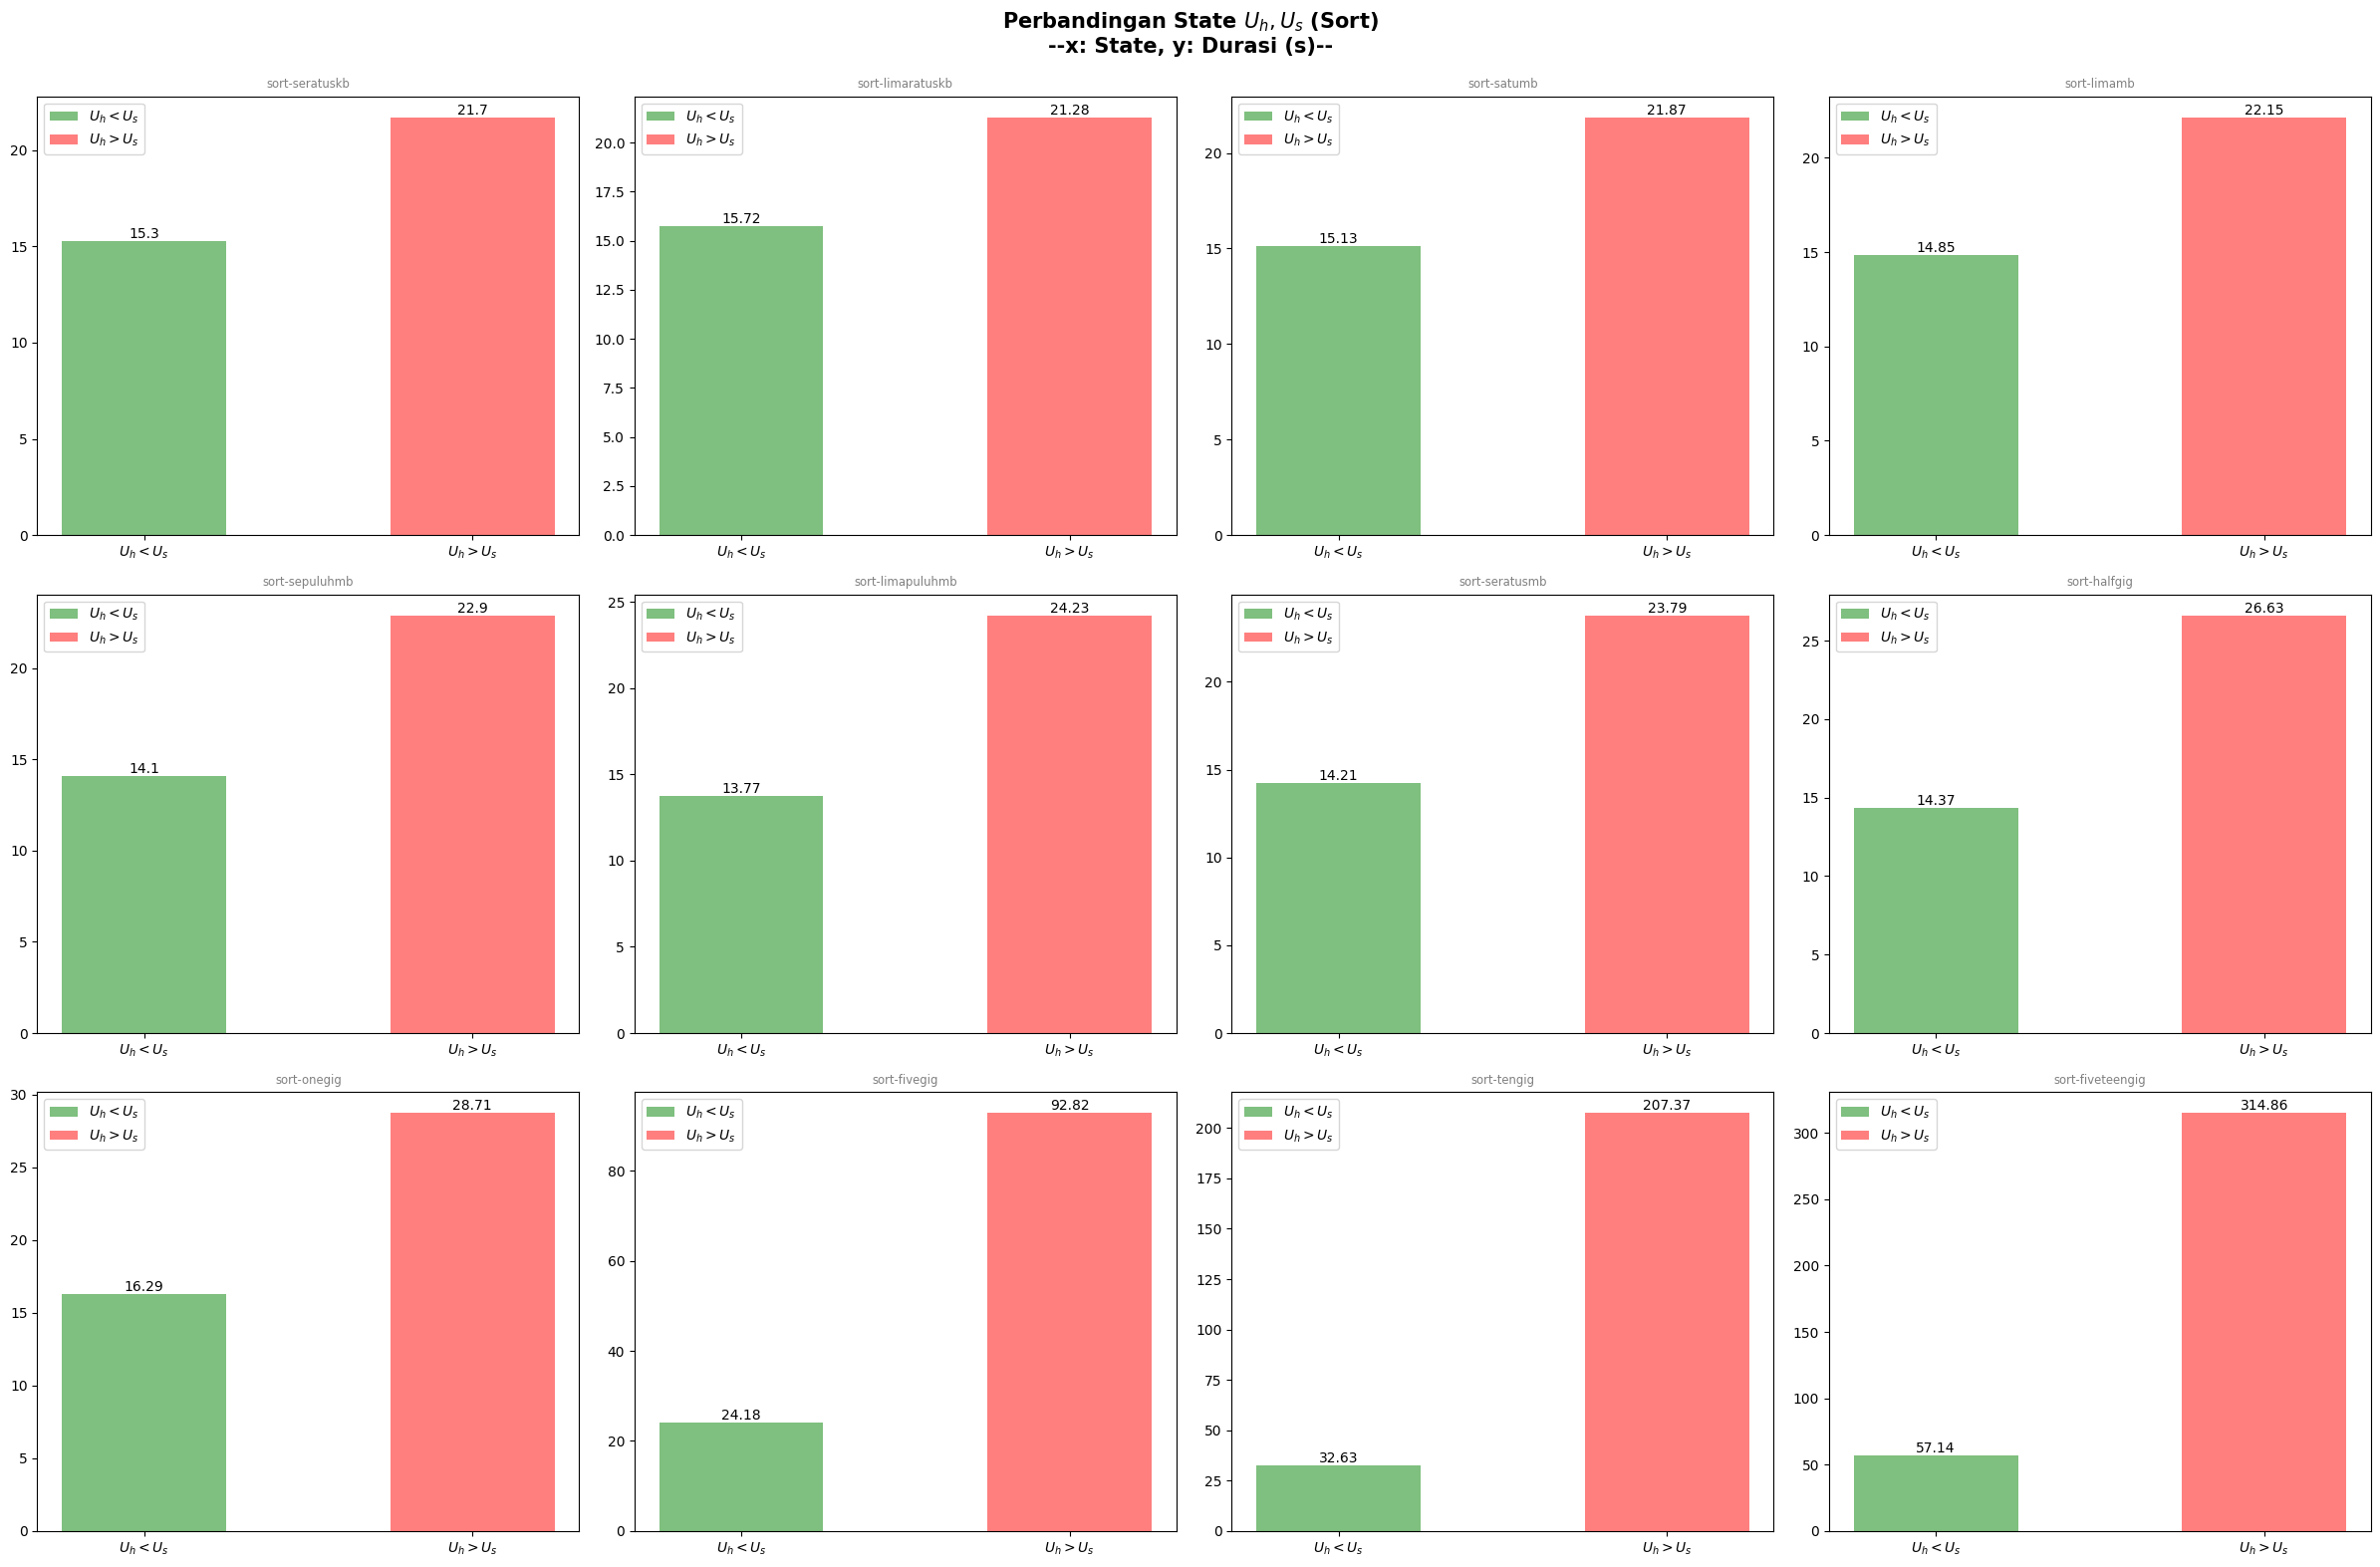
\includegraphics[height=0.6\linewidth]{figures/ch04/4-state-sort.png}
    \caption{Perbandingan \textit{State (Sort)}}
    \label{fig:4-state-sort}
\end{figure}
\end{landscape}

\begin{landscape}
\begin{figure}[h]
    \centering
    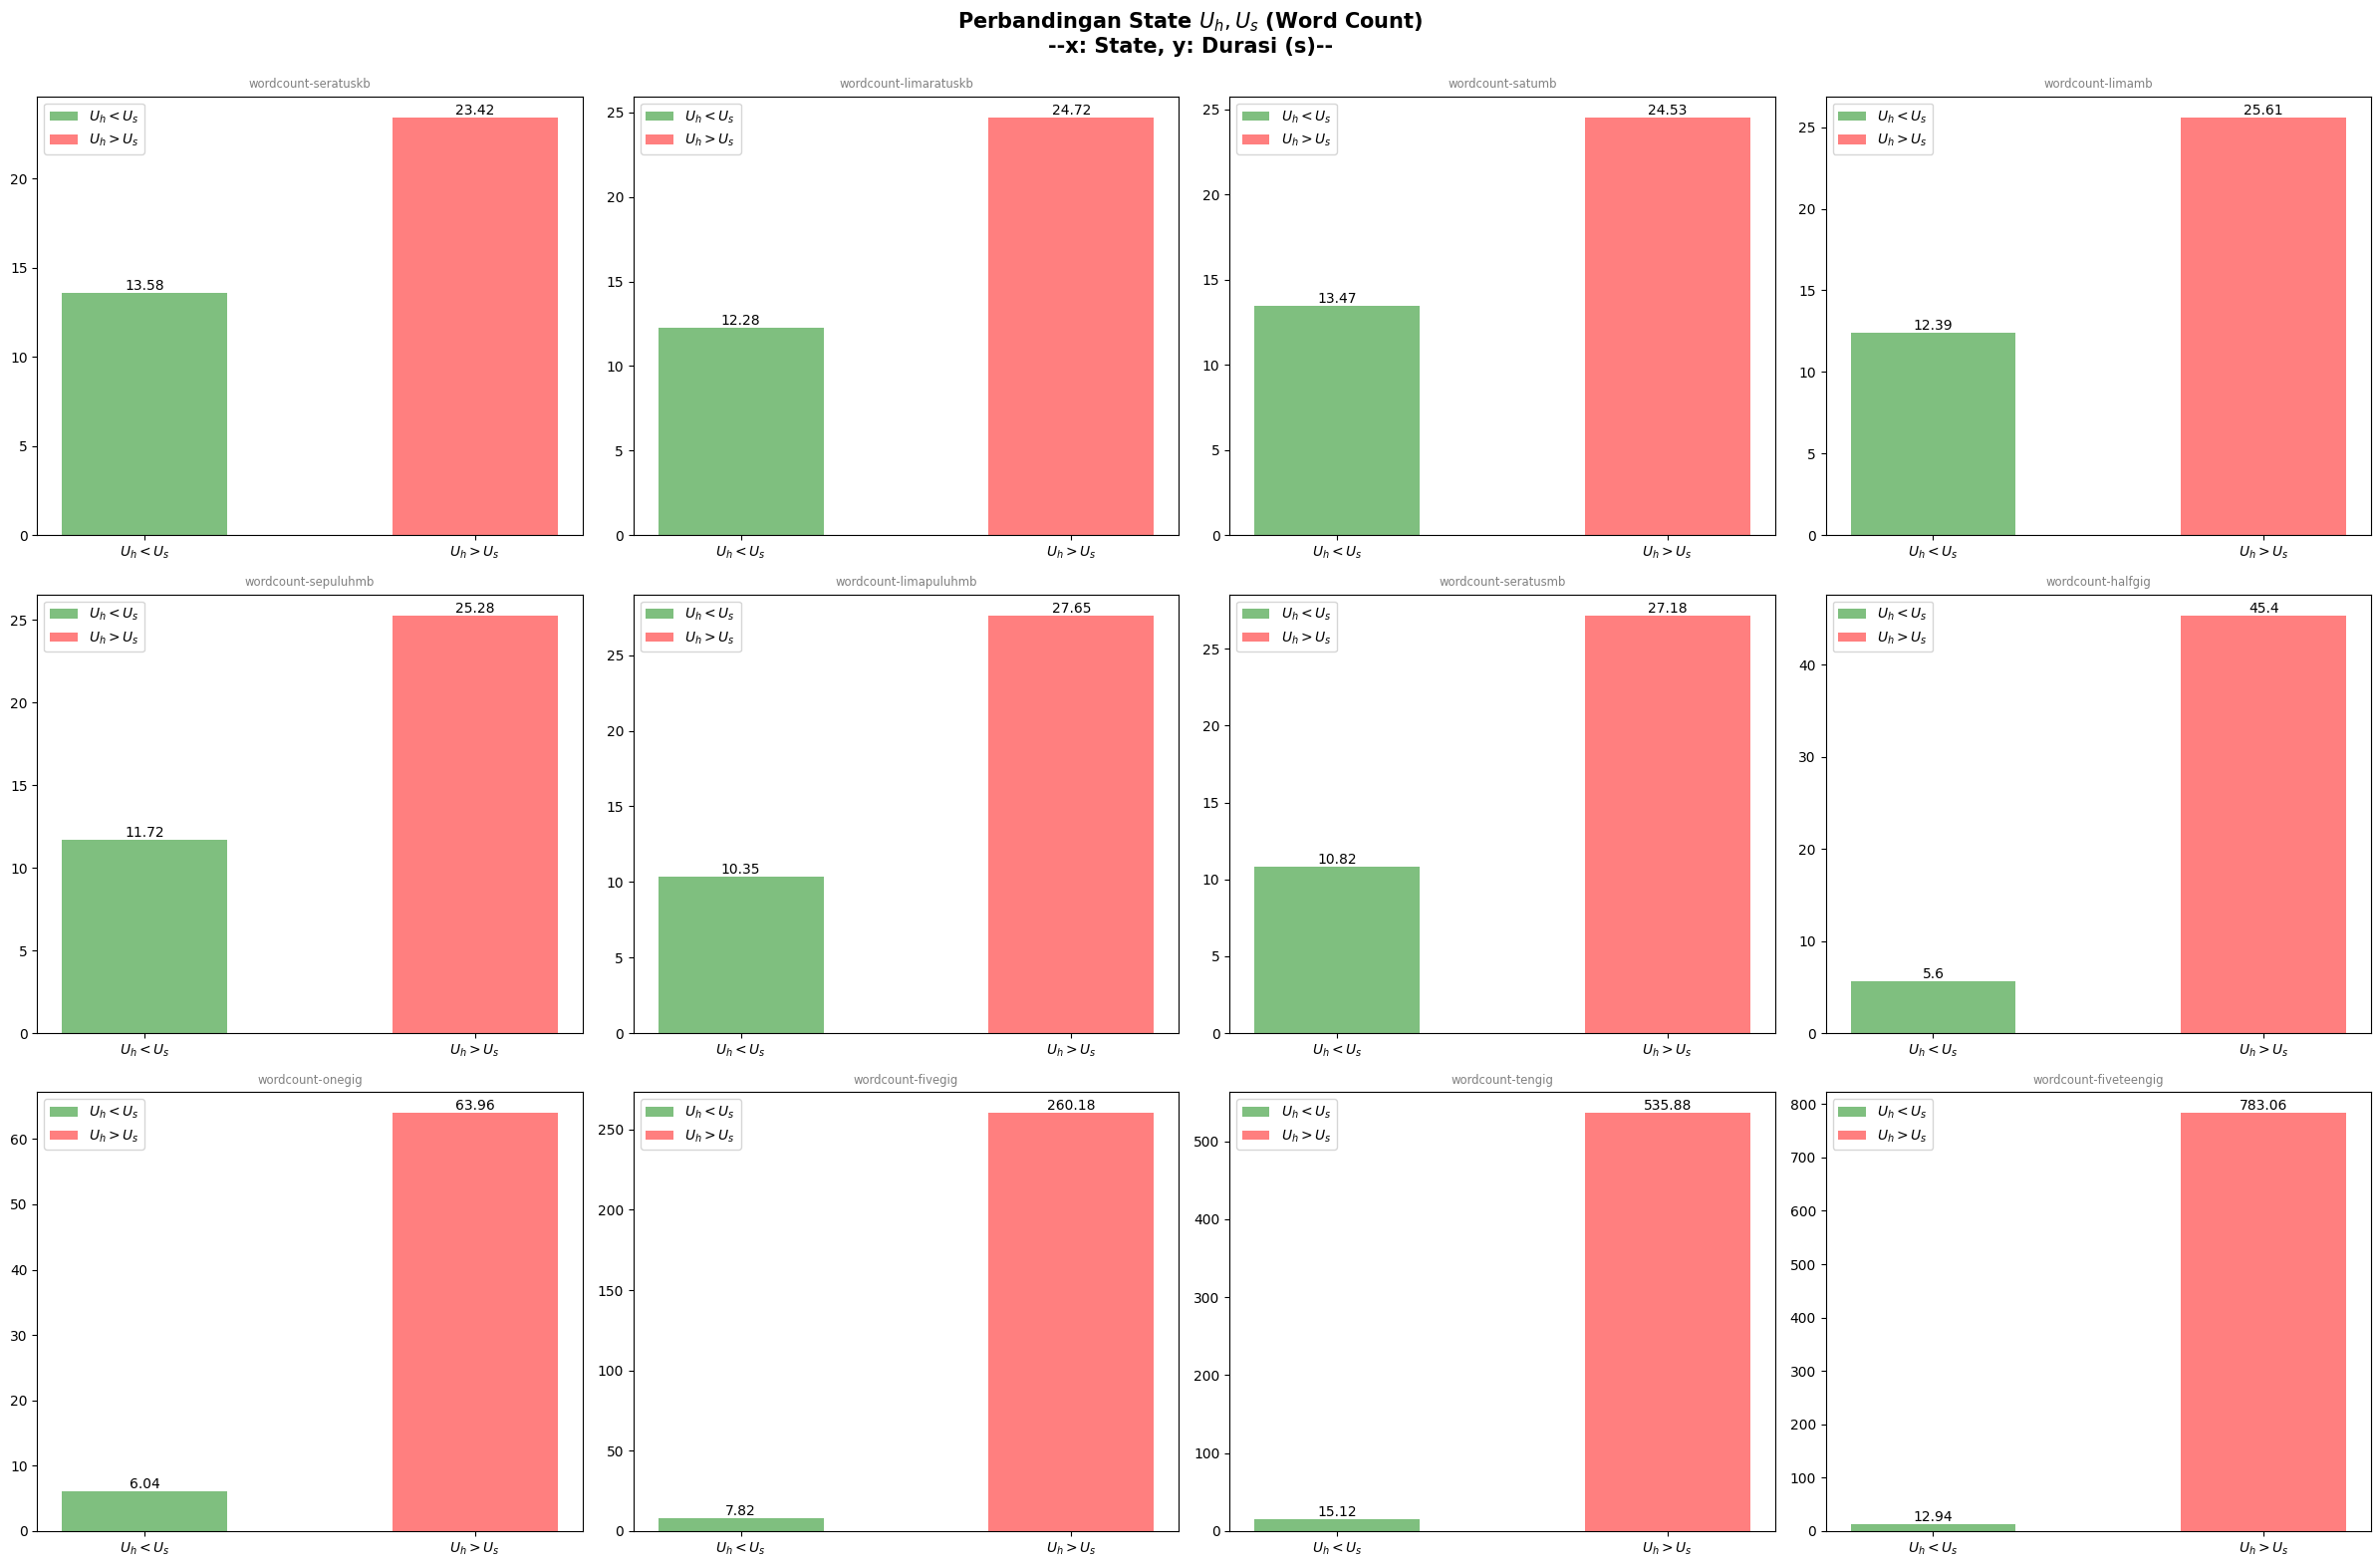
\includegraphics[height=0.6\linewidth]{figures/ch04/4-state-wordcount.png}
    \caption{Perbandingan \textit{State  (Word Count)}}
    \label{fig:4-state-wordcount}
\end{figure}
\end{landscape}

\newpage
\subsection{Utilisasi Sistem}
Utilisasi sistem secara lengkap dapat dilihat pada Lampiran \ref{appendix:G} untuk beban kerja \textit{sort} dan Lampiran \ref{appendix:H} untuk beban kerja \textit{word count}. Setiap gambar akan terdiri dari dua baris dan tiga kolom. Baris pertama berisi visualisasi utilisasi sistem untuk Hadoop dan baris kedua berisi visualisasi untuk Spark. Setiap baris berisi tiga utilisasi sistem, yaitu
\begin{enumerate}
\item Penggunaan CPU (\%)
\item \textit{Disk} I/O (MB)
\item Memori (GB)
\end{enumerate}

Berdasarkan analisis pola penggunaan CPU pada tahap sebelumnya yang menunjukkan bahwa penggunaan CPU Hadoop dan Spark memiliki polanya masing-masing, maka pada tahap ini hanya akan ditampilkan utilisasi sistem pada input data terkecil (100 KB) dan input data terbesar (15 GB).

\begin{figure}[h]
    \centering
    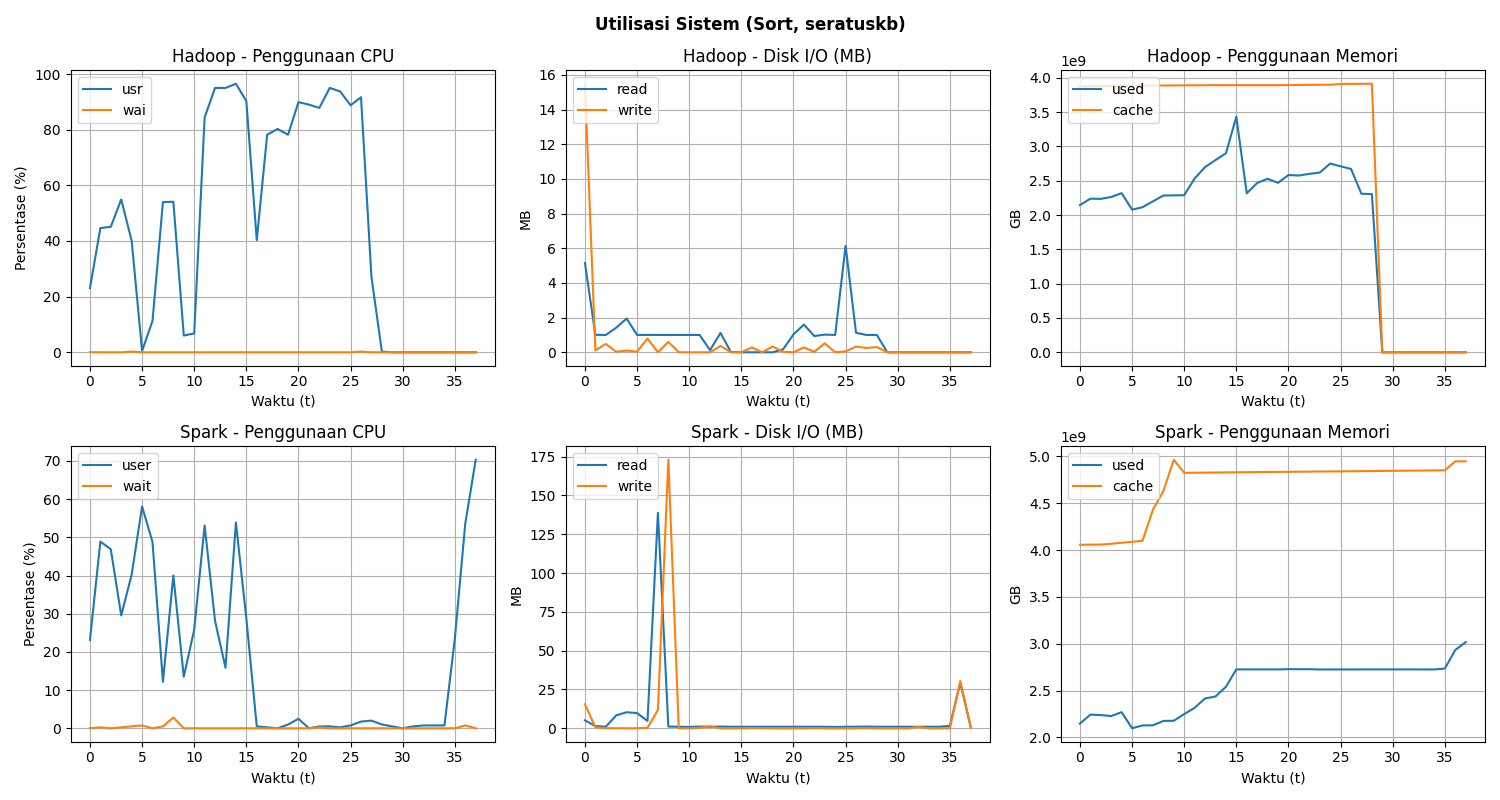
\includegraphics[width=1\textwidth]{figures/ch04/5-util-sistem-sort-seratuskb}
    \caption{Utilisasi Sistem (\textit{Sort}) pada Input Data 100 KB}
    \label{fig:5-util-sistem-sort-seratuskb}
\end{figure}

Pada beban kerja \textit{sort} dan input data sebesar 100 KB (seperti yang ditunjukkan Gambar \ref{fig:5-util-sistem-sort-seratuskb}), Hadoop memiliki penggunaan CPU yang lebih tinggi, yaitu hampir menyentuh 100\%. Sedangkan, pada Spark, penggunaan CPU tertinggi sekitar 70\%. Selanjutnya, ditinjau dari \textit{disk I/O}, aktivitas baca (\textit{read}) dan tulis (\textit{write}) pada Hadoop cenderung lebih sering namun memiliki kecepatan yang lebih lambat dibandingkan dengan Spark. Spark memiliki aktivitas baca tulis yang lebih tinggi, yaitu 140 MB untuk baca dan 175 MB untuk tulis. Kemudian, jika ditinjau dari penggunaan memori, Hadoop dan Spark memiliki penggunaan memori yang tidak berbeda jauh, yaitu sekitar 2 GB-3.5 GB.

\begin{figure}[h]
    \centering
    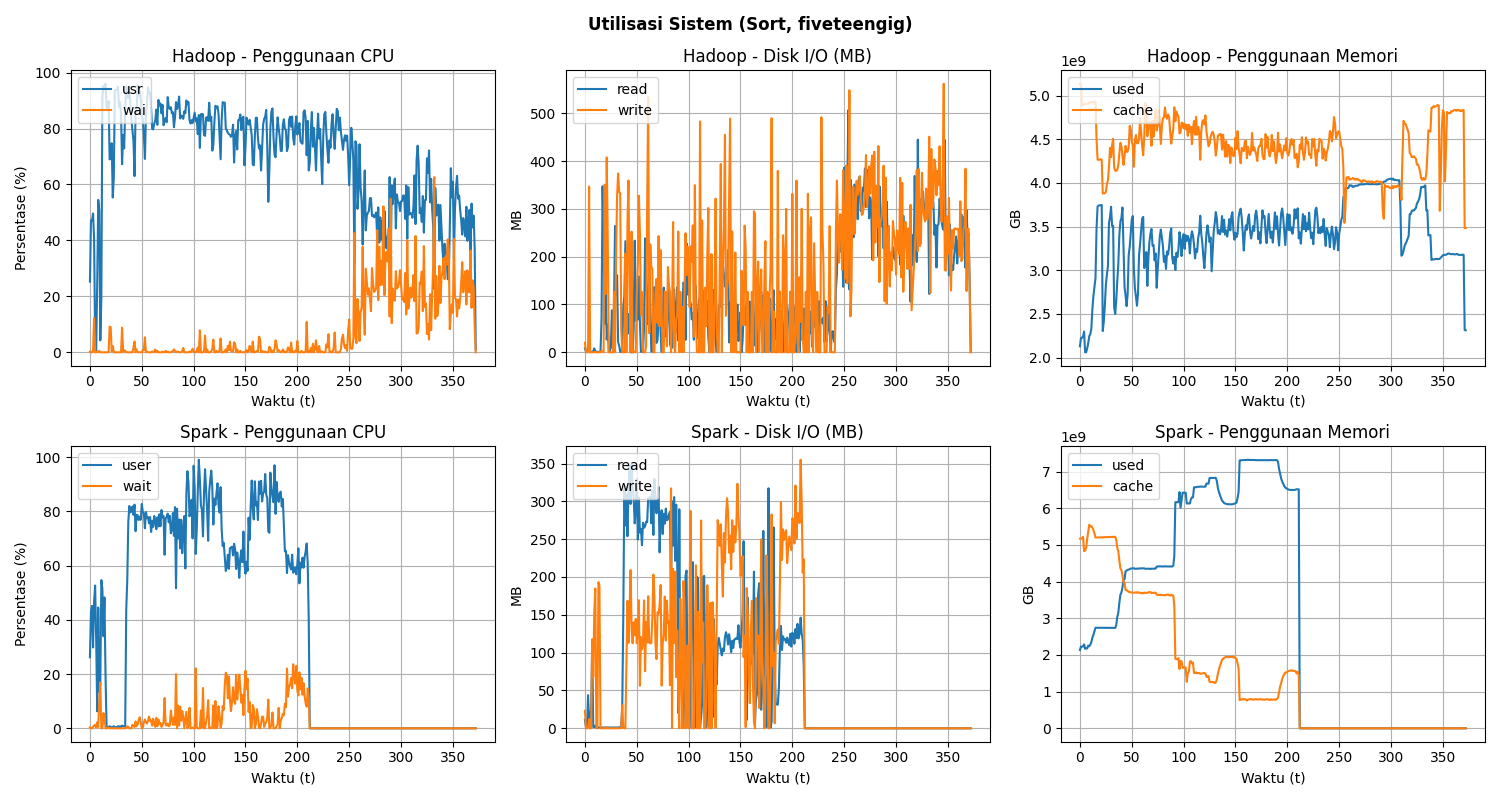
\includegraphics[width=1\textwidth]{figures/ch04/5-util-sistem-sort-fiveteengig}
    \caption{Utilisasi Sistem (\textit{Sort}) pada Input Data 15 GB}
    \label{fig:5-util-sistem-sort-fiveteengig}
\end{figure}

\newpage
Pada beban kerja \textit{sort} dan input data yang lebih besar, yaitu 15 GB (seperti yang ditunjukkan pada Gambar \ref{fig:5-util-sistem-sort-fiveteengig}), utilisasi sistem pada Hadoop dan Spark lebih terlihat jelas perbedaannya. Jika dilihat pada penggunaan CPU, Hadoop membutuhkan waktu penggunaan CPU yang lebih lama, yaitu sekitar 370 detik, dimana Spark hanya membutuhkan waktu sekitar 220 detik. Selanjutnya, Hadoop memiliki penggunaan CPU "\textit{user}" yang lebih stabil, jika dibandingkan dengan Spark yang naik turun secara konstan. Penggunaan CPU "\textit{wait}" akan naik ketika penggunaan CPU "\textit{user}" itu turun. Bergeser pada \textit{disk I/O}, Hadoop memiliki siklus baca tulis yang lebih intensif jika dibandingkan pada Spark. Selanjutnya, jika dilihat dari penggunaan memori, Spark lebih "rakus" akan memori. Hal ini ditandai dengan puncaknya membutuhkan memori sekitar 6-7 GB, dimana Hadoop hanya membutuhkan memori sekitar 3.5 GB.

\begin{figure}[h]
    \centering
    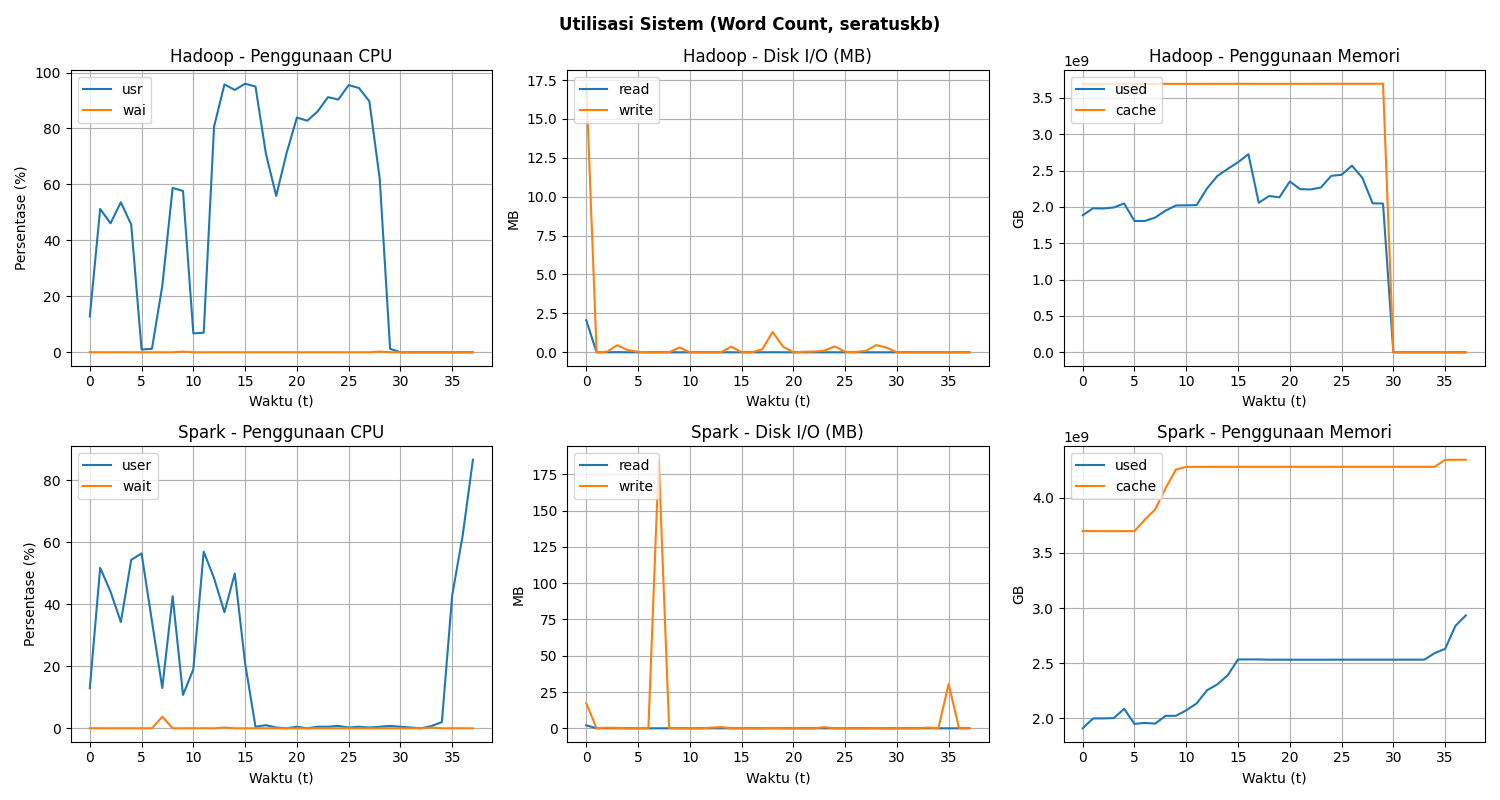
\includegraphics[width=1\textwidth]{figures/ch04/5-util-sistem-wordcount-seratuskb}
    \caption{Utilisasi Sistem (\textit{Word Count}) pada Input Data 100 KB}
    \label{fig:5-util-sistem-wordcount-seratuskb}
\end{figure}

Selanjutnya beban kerja \textit{word count}. Pada beban kerja \textit{word count} dengan input data 100 KB, pola yang didapatkan untuk penggunaan CPU, \textit{disk I/O}, dan penggunaan memori tidak berbeda jauh dengan beban kerja \textit{sort} dengan ukuran input data yang sama. 

\begin{figure}[h]
    \centering
    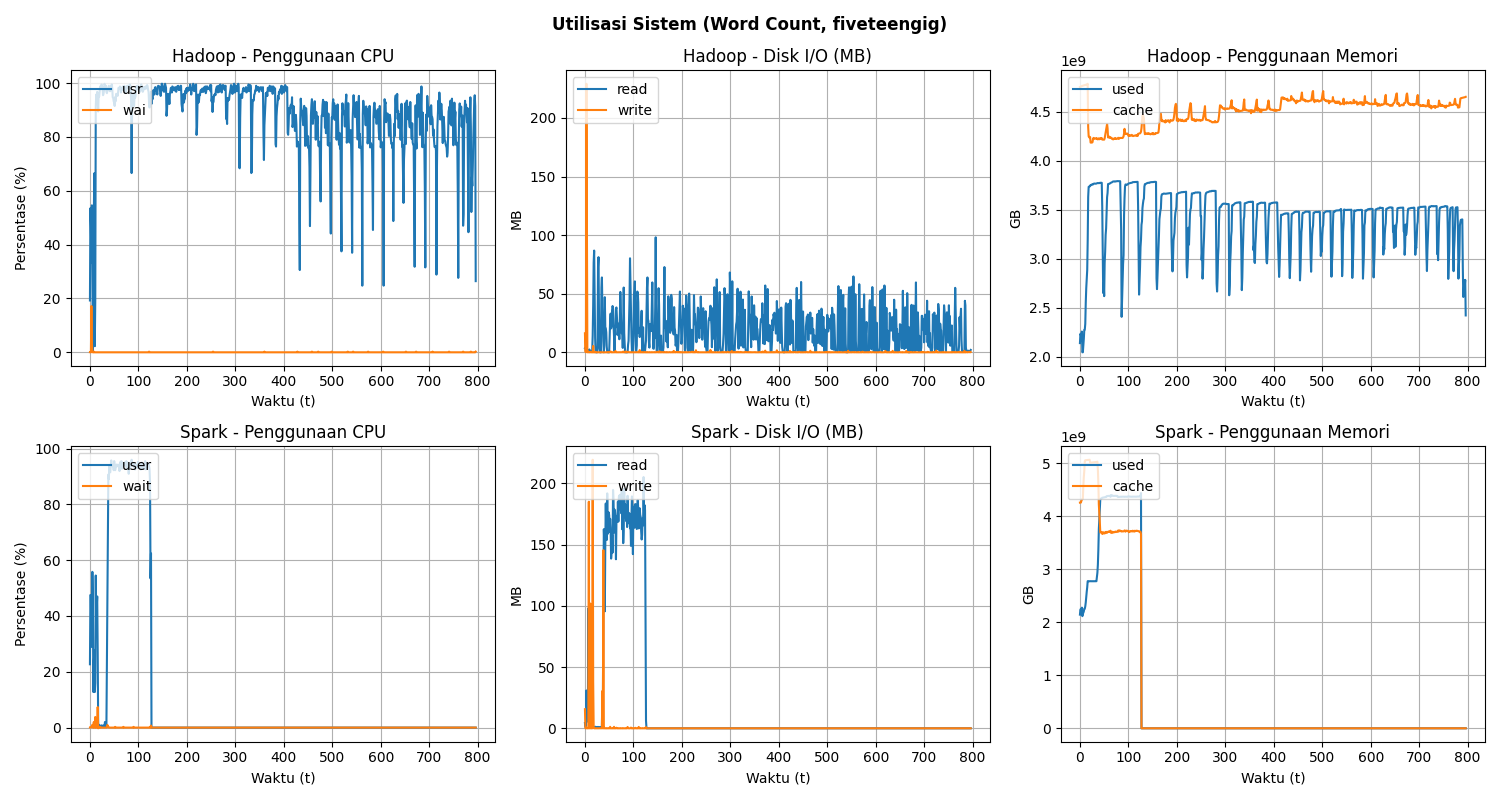
\includegraphics[width=1\textwidth]{figures/ch04/5-util-sistem-wordcount-fiveteengig}
    \caption{Utilisasi Sistem (\textit{Word Count}) pada Input Data 15 GB}
    \label{fig:5-util-sistem-wordcount-fiveteengig}
\end{figure}

Pada beban kerja \textit{word count} dan input data yang lebih besar, yaitu 15 GB (seperti yang ditunjukkan pada Gambar \ref{fig:5-util-sistem-wordcount-fiveteengig}), utilisasi sistem pada Hadoop dan Spark lebih terlihat jelas perbedaannya. Pada penggunaan CPU, Hadoop memiliki aktivitas penggunaan yang lebih tinggi dan lebih konstan sampai akhir waktu eksekusi. Hal ini berbeda dengan Spark yang hanya butuh waktu sekitar 150 detik saja dengan penggunaan CPU yang hanya 90\%. Selanjutnya, pada aktivitas baca tulis (\textit{disk I/O}), Hadoop memiliki aktivitas baca yang lebih intensif (sepanjang waktu eksekusi) dengan sedikit aktivitas tulis (pada awal waktu eksekusi). Aktivitas baca yang dilakukan oleh Hadoop berada pada ukuran 50-100 MB setiap waktunya. Pada Spark, aktivitas baca tersebut berukuran 150-200 MB. Kemudian, jika ditinjau melalui penggunaan memori, memori yang dibutuhkan Hadoop berkisar pada 2.5-3.7 GB. Pada Spark, memori yang dibutuhkan berkisar pada 2-4.5 GB.  

Hadoop menunjukkan aktivitas \textit{Disk} I/O yang jauh lebih tinggi dibandingkan dengan Spark, terutama pada beban kerja \textit{sort}. Grafik \textit{Disk} I/O Hadoop menunjukkan lonjakan aktivitas baca dan tulis yang signifikan sepanjang waktu eksekusi. Hal ini sesuai dengan pendekatan berbasis disk Hadoop yang membutuhkan pembacaan dan penulisan data ke \textit{disk} secara intensif. Sebaliknya, Spark, dengan arsitektur in-memory, meminimalkan operasi \textit{Disk} I/O. Grafik \textit{Disk} I/O Spark menunjukkan aktivitas yang jauh lebih rendah dan stabil, yang berkontribusi pada peningkatan performanya.

Spark menunjukkan penggunaan memori yang lebih tinggi dan stabil dibandingkan dengan Hadoop, terutama pada beban kerja \textit{sort}. Grafik penggunaan memori Spark menunjukkan garis yang cenderung mendatar pada tingkat utilisasi yang tinggi, menunjukkan bahwa Spark menyimpan data dalam RAM untuk akses yang lebih cepat dan pemrosesan yang efisien. Penggunaan memori Hadoop lebih rendah dan fluktuatif, menunjukkan bahwa Hadoop tidak memanfaatkan memori secara optimal. 

Analisis pemantauan sistem menegaskan keunggulan Spark dalam hal efisiensi dan optimasi penggunaan sumber daya komputasi dibandingkan dengan Hadoop. Spark mampu memaksimalkan penggunaan CPU, meminimalkan operasi \textit{Disk} I/O, dan memanfaatkan memori secara efisien, yang berkontribusi pada performa dan skalabilitas yang lebih baik dalam tugas-tugas pemrosesan data besar.

\section{Perbandingan dengan Penelitian Sebelumnya}
Penelitian terdahulu yang melakukan perbandingan Hadoop dan Spark menggunakan HiBench telah mendapatkan hasil seperti pada Gambar \ref{fig:0-penelitian-lama}. Pada gambar tersebut terlihat bahwa pada input data 1 GB dan pada beban kerja \textit{word count}, terjadi peningkatan performa sebesar tiga kali lipat, pada input data 5 GB sebesar 3.5 lipat, dan begitu juga pada input data 10 GB.

\begin{figure}[h]
    \centering
    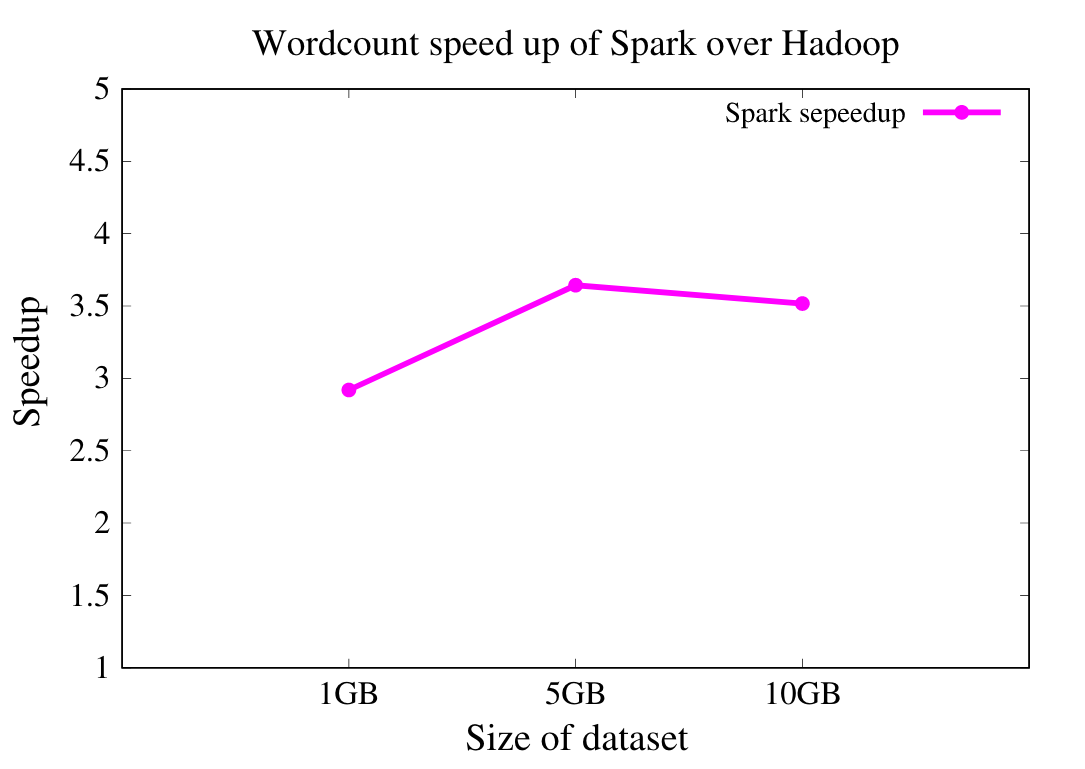
\includegraphics[width=1\textwidth]{figures/ch04/0-penelitian lama}
    \caption{Rasio Peningkatan Performa Spark-Hadoop Berdasarkan Input Data \cite{samadiPerformanceComparisonHadoop2018}}
    \label{fig:0-penelitian-lama}
\end{figure}

Penelitian ini menghasilkan hasil yang serupa, seperti yang ditunjukkan pada Tabel \ref{table:penelitian-baru}. Pada penelitian ini, rasio peningkatan performa naik secara bertahap dari input data 1 GB, 5 GB, 10 GB, hingga 15 GB. Hal ini dapat terjadi karena adanya perbedaan konfigurasi perangkat keras dan perbedaan versi perangkat lunak yang digunakan.

\begin{table}[h]
  \centering
  \caption{Rasio Peningkatan Performa Spark-Hadoop Berdasarkan Input Data (Baru)}
  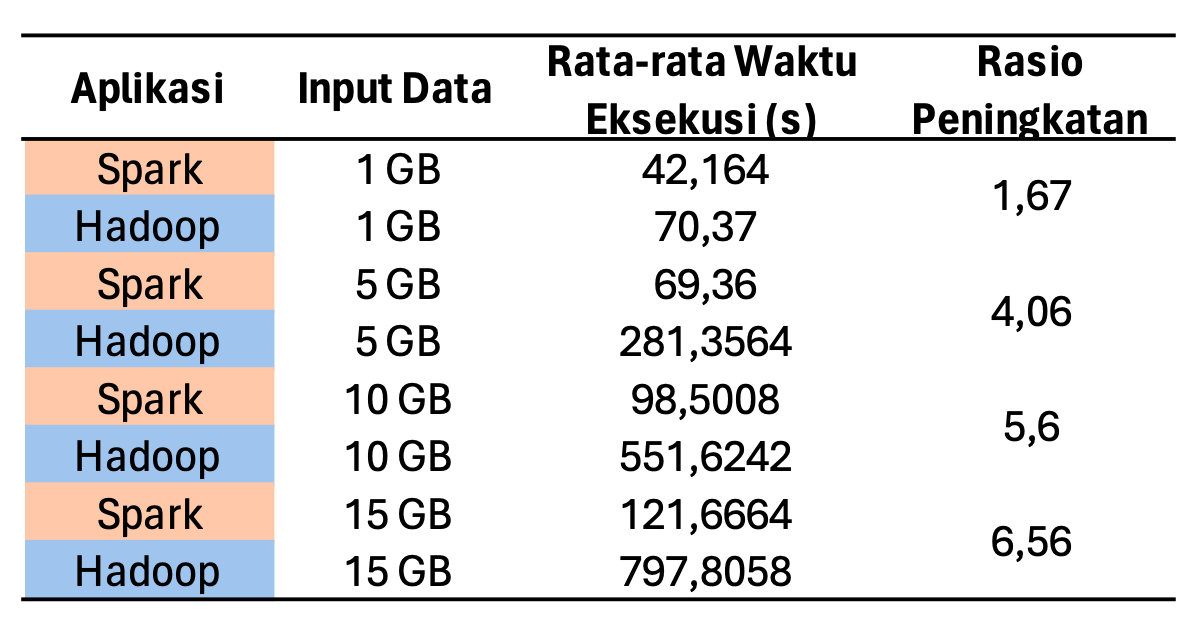
\includegraphics[width=0.8\textwidth]{figures/ch04/0-penelitian-baru}
  \label{table:penelitian-baru}
\end{table}

Pada Tabel \ref{table:penelitian-baru}, dapat dilihat bahwa Spark menunjukkan peningkatan performa yang signifikan dibandingkan Hadoop pada berbagai ukuran input data. Pada input data 1 GB, Spark memiliki rasio peningkatan sebesar 1.67 kali lipat dibandingkan Hadoop. Pada input data 5 GB, rasio peningkatan naik menjadi 4.06 kali lipat. Begitu juga dengan input data 10 GB dan 15 GB, rasio peningkatannya masing-masing sebesar 5.6 kali lipat dan 6.56 kali lipat.

Secara keseluruhan, hasil penelitian ini konsisten dengan penelitian sebelumnya, namun menunjukkan peningkatan performa yang lebih signifikan pada ukuran data yang lebih besar. Hal ini menunjukkan bahwa Spark lebih efisien dalam menangani data dalam skala besar dibandingkan Hadoop, terutama pada beban kerja \textit{word count}.


